\documentclass[10pt]{article}
\def\baselinestretch{1.1}
\usepackage[bookmarks]{hyperref}
\usepackage{kotex} % korean tex
\usepackage[utf8]{inputenc} % set input encoding (not needed with XeLaTeX)

\usepackage{geometry} % to change the page dimensions
\geometry{letterpaper} % or letterpaper (US) or a5paper or....
% \geometry{margins=2in} % for example, change the margins 
%to 2 inches all round
% \geometry{landscape} % set up the page for landscape
%   read geometry.pdf for detailed page layout information

\usepackage{graphicx} % support the \includegraphics command and options

% \usepackage[parfill]{parskip} % Activate to begin paragraphs 
%with an empty line rather than an indent

\usepackage{booktabs} % for much better looking tables
\usepackage{array} % for better arrays (eg matrices) in maths
\usepackage{paralist} % very flexible & customisable lists 
%(eg. enumerate/itemize, etc.)
\usepackage{verbatim} % adds environment for commenting 
% out blocks of text & for better verbatim
\usepackage{subfig} % make it possible to include 
%more than one captioned figure/table in a single float
% These packages are all incorporated in the memoir class 
%to one degree or another...

%%% HEADERS & FOOTERS
\usepackage{fancyhdr} % This should be set 
% AFTER setting up the page geometry
\pagestyle{fancy} % options: empty , plain , fancy
\renewcommand{\headrulewidth}{0pt} % customise the layout...
\lhead{}\chead{}\rhead{}
\lfoot{}\cfoot{\thepage}\rfoot{}

%%% SECTION TITLE APPEARANCE
\usepackage{sectsty}
\allsectionsfont{\sffamily\mdseries\upshape} 
% (See the fntguide.pdf for font help)
% (This matches ConTeXt defaults)

%%% ToC (table of contents) APPEARANCE
\usepackage[nottoc,notlof,notlot]{tocbibind} 
% Put the bibliography in the ToC
\usepackage[titles,subfigure]{tocloft} 
% Alter the style of the Table of Contents
\renewcommand{\cftsecfont}{\rmfamily\mdseries\upshape}
\renewcommand{\cftsecpagefont}{\rmfamily\mdseries\upshape} % No bold!

\usepackage{amsmath}
\usepackage{amssymb}
\usepackage{epsfig}
\usepackage{color}

\usepackage{empheq}
% make possible to box equations, For example
%\begin{empheq}[box=\fbox]{align*}
%a&=b \tag{test}\\
%E&=mc^2 + \int_a^a x\, dx
%\end{empheq}

\parindent 10pt\textheight 9in\topmargin -0.4in\textwidth 6in
\oddsidemargin .25in\evensidemargin 0in
\def\bm{\boldsymbol}
\newcommand{\bea}{\begin{eqnarray}}
\newcommand{\eea}{\end{eqnarray}}
\newcommand{\be}{\begin{eqnarray}}
\newcommand{\ee}{\end{eqnarray}}
\newcommand{\no}{\nonumber \\}
\newcommand{\nnb}{\nonumber}
\newcommand{\etal}{{\it et al.}~}
\newcommand{\eg}{{\it e.g.}}
\newcommand{\ie}{{\it i.e.}}
\newcommand{\sll}[1]{#1\hspace{-0.5em}/}
\newcommand{\del}{\partial}
\def\vs{{\bm \sigma}}
\def\vh{{\bm h}}
\def\vp{{\bm p}}
\def\vq{{\bm q}}
\def\vk{{\bm k}}
\def\vl{{\bm l}}
\def\vx{{\bm x}}
\def\vy{{\bm y}}
\def\vv{{\bm v}}
\def\vr{{\bm r}}
\def\vR{{\bm R}}
\def\la{\langle}
\def\ra{\rangle}
\newcommand{\threejsymbol}[6]
{\left(\begin{tabular}{ccc} {$#1$}&{$#2$}&{$#3$}\\
                             {$#4$}&{$#5$}&{$#6$}\end{tabular}\right)}
\newcommand{\sixjsymbol}[6]
{\left\{\begin{tabular}{ccc} {$#1$}&{$#2$}&{$#3$}\\
                             {$#4$}&{$#5$}&{$#6$} \end{tabular}\right\}}


%%% The "real" document content comes below...

\title{Scattering Theory Note: Two body}
\author{Young-Ho Song}
\date{\today}
%\date{} % Activate to display a given date or no date (if empty),
         % otherwise the current date is printed 

\begin{document}
\maketitle
\tableofcontents
\newpage

The basic object of this note is to summarize basic 
relations between scattering
observables(or phase shift, t-matrix) and potentials. 
And also the algorithm
to solve the two-body scattering problem. We will use 
time-independent formalism. 

\section{Basic terminology and Kinematics}
\label{sec:1}
\begin{itemize}
\item 일반적인 two-body problem can be decomposed as 
center of mass kinetic energy and two-body relative 
motion.
\bea
\la \vr_1 \vr_2|H|\vr'_1\vr'_2\ra
=\la \vR \vr|H|\vR' \vr'\ra
=\delta^{(3)}(\vR-\vR')
 \left[
 \delta^{(3)}(\vr-\vr')\left(-\frac{\nabla^2_R}{2M_{tot}}
                       -\frac{\nabla_r^2}{2\mu}\right)
 +V(\vr,\vr')\right]                      
\eea

C.M. frame 에서,
scattering 에너지는 two-body 의 relative kinetic energy 이고,
$E=\frac{\vk^2}{2\mu}$ with reduced mass 
$\mu=\frac{m_1m_2}{m_1+m_2}$로 나타내진다. 
\footnote{
주의: $\vk_{rel}\equiv \mu v_{rel} \neq \vp_1-\vp_2$.}
\footnote{
{\bf 주의: state나 matrix element를 나타낼 때,
$|\vk\ra$, $|k, \alpha\ra$, $|\alpha\ra$ 는 각각
다른 의미를 가진다. $|\vk\ra$는 plane wave, $|k,\alpha\ra$ 는
partial wave with radial wave function, $|\alpha\ra$는 
angular part without radial wave function.}
}

\item Non-relativistic kinematics: 

$m_1$ and $m_2$ particles in c.m. frame and
$m_2$ is rest in lab frame.
In relativistic expression,
\bea
(m_2+\sqrt{m_1^2+\vp_1^2})^2-\vp_1^2 
       =(\sqrt{m_1^2+\vp_c^2}+\sqrt{m_2^2+\vp_c^2})^2,
\eea
where $\vp_{1}$ is momentum in Lab. frame, $\vp_c$ is momentum in
C.M. frame. Solving this equation gives a relation between,
$\vp_1$ and $\vp_c$. In terms of kinetic energy,
\bea
(m_1+m_2+T^L)^2-(T^L+m_1)^2+m_1^2
=(m_1+m_2+T^C)^2,
\eea
gives the relation between $T^L$ and $T^C$.
\footnote{In case $m_1=m_2$, $T^L=2 T^C+\frac{(T^{C})^2}{2m}$}

On the other hand, the definition of 
$\vk_{rel}=\mu{\bf v}_{rel}$ and non-relativistic expression,
${\bf v}_{rel}=\frac{\vp_1}{m_1}-\frac{\vp_2}{m_2}$ gives
$\frac{\vk_{rel}}{\mu}=\frac{\vp_1}{m_1}$ in lab frame.
Also in c.m. frame, 
$\vk_{rel}=\mu(\frac{\vp_c}{m_1}-\frac{-\vp_c}{m_2})=\vp_c$.
In non-relativistic approximation,
\bea
& &T^L=\frac{\hbar^2}{2m_1}\vp^2,\quad T^C=\frac{\hbar^2}{2\mu}\vk^2,
\quad \mu=\frac{m_1 m_2}{m_1+m_2},\no
& &\hbar{\vp}_1=m_1{\bm v}_{rel},\quad
\hbar\vk=\mu{\bm v}_{rel}=m_1{\bm v}_{1c}=-m_2{\bm v}_{2c},
\quad {\bm v}_{rel}={\bm v}_1-{\bm v}_2,
\no
& &
 T^L=\frac{m_1}{2}{\bm v}_{rel}^2=\frac{m_1}{\mu}T^c
\eea

Let us always use only $\mbox{fm}$ as a fundamental units. Other quantities are always converted by using
$\hbar=c=1$ and $\hbar c=1=197 \mbox{MeV}.\mbox{fm}$.



\end{itemize}

\subsection{Normalization convention}

In c.m. frame $E_k=\frac{\vk^2}{2\mu}$
with $\vk=\mu {\bm v}_{rel}$ relative momentum
between two cluster, $\mu$ reduced mass.
\footnote{
$\int d\vx |\vx\ra \la \vx|=1, \quad \la \vx|\vx'\ra
=\delta^{(3)}(\vx-\vx')$ 은 어느 경우나 공통이다.
}
\bea
\la \vx|\vk\ra&\equiv&\frac{1}{(2\pi)^\frac{3}{2}}e^{i\vk\cdot\vx}
\no
\int d\vk |\vk\ra \la \vk|&=&1, \quad \la \vk'|\vk\ra=\delta^{(3)}(\vk-\vk')
\eea
(Sakurai book, Rimas 논문, Glockle 의 책은 이 convention을 사용한다.)
반면에, Another popular convention 
$\la \vk|\vk'\ra=(2\pi)^3\delta^3(\vk-\vk')$ 으로 정의할 경우엔 
\bea
\la \vx|\vk\ra&=&e^{i\vk\cdot\vx},\no 
\int \frac{d\vk}{(2\pi)^3} |\vk\ra \la \vk|&=&1, 
\quad \la \vk'|\vk\ra=(2\pi)^3 \delta^{3}(\vk-\vk')
\eea
이 된다. 이 노트에서는 앞의 normalization 즉, $\la \vk'|\vk\ra=\delta^3(\vk-\vk')$을
사용하기로 하자.
\footnote{ high energy 에서는 state를 4-vector로
생각하고,
\bea
\la k^\mu | k^{'\mu}\ra=(2\pi)^4(2E_k)\delta^{(4)}(k-k')
\eea
로 정하는 것이 편리하고, 이 때는 energy conservation을
$(2\pi)\delta(k^0-k^{'0})$로 뽑아내는 것이 편리하다. }


\subsection{Formal scattering theory: In-, Out- state and Moller operator}
Scattering 은 흔히 free incoming state 로부터 
free outgoing state 로의 변화를 나타낸다.\footnote{
scattering theory에서 사용하는 potential이 만족해야하는 조건은 
흔히  (1) $V(r)$ 은 large r에 대해 $r^{-3}$ 보다 빨리 떨어져야 한다. 
(2) $V(r)$은 small r에서 $r^{-2}$ 보다 덜 singular 해야한다.
(3) $V(r)$은 continuous 해야 한다. 

따라서, Coulomb potential이나 attractive singular potential의 경우에는 
다른 formalism을 사용해야 한다. 
}
따라서, 이 둘을 연결시켜 주는 S operator(scattering operator)를 
\bea
|\psi_{out}\ra=S|\psi_{in}\ra
\eea
을 생각할 수 있다. 

We can consider $|\psi_{in}\ra$ state such that 
time evolution of $|\psi\ra$ at $t=0$ state becomes

\bea
& &U(t)|\psi\ra \to_{t\to -\infty}  U^0(t)|\psi_{in}\ra ,\no
& &U(t)|\psi\ra \to_{t\to +\infty}  U^0(t)|\psi_{out}\ra.
\eea
where $U(t)=e^{-iH t}$ and $U_0(t)=e^{-iH_0 t}$. Thus,

M\"{o}ller operator $\Omega_{\pm}$ 를 다음과 같이 정의할 수 있다.
\bea
\Omega_{\pm}&\equiv&\lim_{t\to \mp\infty} U(t)^\dagger U_0(t),\no
|\psi\ra&=&\Omega_{+}|\psi_{in}\ra=\Omega_{-}|\psi_{out}\ra
\eea

  
\begin{equation}
\boxed{
\begin{array}{ccccc}
\mbox{in asymptote} & \rightarrow^{\Omega_+} & \mbox{actual state at t=0}
                    & \leftarrow^{\Omega_-}  & \mbox{ out asymptote}\\
|\psi_{in}\ra       & \rightarrow            & |\psi\ra 
                    &\leftarrow              & |\psi_{out}\ra\\
|\phi\ra            &\rightarrow             &|\phi+\ra
                    &                        &  \\
                    &                        & |\chi-\ra
                    & \leftarrow             & |\chi\ra\\       
\end{array}
}
\end{equation}
where, $|\phi+\ra$ means the actual state of the system at $t=0$
{\it if the in asymptote was $|\phi_{in}\ra=|\phi\ra$}.
(It does not mean state at $t\to +\infty$.)
\footnote{$\Omega_{+}|\phi\ra\equiv |\phi+\ra$,
$\Omega_{-}|\chi\ra\equiv |\chi-\ra$.}


S-matrix는  
\bea
S=\Omega^\dagger_{-}\Omega_{+}=1+R \mbox{ or } 1-R
\eea
로 정의 될 수 있고, Unitary 임을 알 수 있다. 
Probability is related with
\bea
w(\chi\leftarrow \phi)=|\la\chi|S|\phi\ra|^2.
\eea

앞으로 
$|\vk\ra$와 $|\vk\ra^{(\pm)}$는 free LS equation과 
full LS equation의 solution이다. 즉,
\bea
H_0|\vk\ra&=&E_k|\vk\ra\no
H|\vk\ra^{(\pm)}&=&(H_0+V)|\vk\ra^{(\pm)}=E_k|\vk\ra^{(\pm)}.
\eea
여기서, $\pm$는 서로 다른 boundary condition을 만족하는 해 임을 
나타낸다.


\section{LS equation for scattering}
\begin{itemize}
\item
From the Shrodinger equation for scattering wave function,
\bea
& &H_0|\vk\ra=E_k|\vk\ra,\no
& &H|\vk\ra^{(\pm)}=(H_0+V)|\vk\ra^{(\pm)} = E_k |\vk\ra^{(\pm)}
\eea
위 식은 LS eq.으로 바꿔 쓸 수 있다. 단, $\frac{1}{E-H_0}$는 
real axis 에서 잘 정의 되는 함수가 아니므로, $\pm i\epsilon$
을 도입하여,
\bea
\boxed{
|\vk\ra^{(\pm)}=|\vk\ra+\frac{1}{E-H_0\pm i\epsilon}V|\vk\ra^{(\pm)},}
\eea
이고, $\pm$는 각각 서로 다른 boundary consition을 준다.
이 식에서  
$H_0$ 는 free particle state $|\vk\ra$에 작용할 때,  $E_k=\frac{\vk^2}{2\mu}$ 이고, 
$E$ is an energy of $|\vk\ra^+$ which 
need not necessarily  be $H_0=\frac{\vk^2}{2\mu}$ 
for relative two-body. However, elastic scattering case, $E_k$ will be the same as $H_0$.

\item Green's function or resolvant : Green function( free resolvant or free propagator) is defined as
\bea
G(z)\equiv\frac{1}{z-H},\quad
G_0(z)\equiv\frac{1}{z-H_0}
\eea
This satisfies (LS equation for Green function) 
\bea
G(z)=G_0(z)+G_0(z)VG(z)
\eea
for $z=E\pm i\epsilon$. Or we can define,
\bea
G^{\pm}(E)=G(E\pm i\epsilon)
\eea
\item {\bf LS equation for scattering state} From above Green's functions,  we obtain $LS$ equation,
\bea
|\vk\ra^{(\pm)}&=&\lim_{\epsilon\to 0} 
       \pm i\epsilon[G_0(E\pm i\epsilon)
                             +G_0(E\pm i\epsilon)V G(E\pm i\epsilon)]|\vk\ra\no 
       &=&|\vk\ra+G_0(E\pm i\epsilon)V|\vk\ra^{(\pm)}
\eea
where, 
\bea
|\vk\ra&=&\lim_{\epsilon\to 0}\frac{\pm i\epsilon}{E_k\pm i\epsilon-H_0}|\vk\ra ,\quad \mbox{Because $H_0|\vk\ra=E_k|\vk\ra$,}\no 
|\vk\ra^{(\pm)}&=&\lim_{\epsilon\to 0}\frac{\pm i\epsilon}{E_k\pm i\epsilon-H}|\vk\ra=(1+\lim_{\epsilon\to 0}\frac{1}{E_k\pm i\epsilon-H} V)|\vk\ra\no
   &=&\lim_{\epsilon\to 0} (\pm i\epsilon) G(E+i\epsilon)|\vk\ra
\eea
are used. 여기서, 
$H_0|\vk\ra=E_k|\vk\ra$, $H|\vk'\ra^{(\pm)}=E_{k'}|\vk'\ra^{(\pm)}$, but 
$H|\vk\ra$ need not be $E_k$임에 주의.


\item 
위 식에서는 Schrodinger eq으로 부터 시작하였지만, 
Moller operator를 이용하여, 같은 결과를 얻을 수 있다.
\bea
|\vk\ra^{(\pm)}&=&\Omega_{\pm}|\vk\ra
       =\lim_{t\to \mp\infty} U(t)^\dagger U_0(t)|\vk\ra\no 
       &=&\lim_{\epsilon\to 0}\pm\frac{\epsilon}{\hbar}
       \int^0_{\mp\infty} dt
       e^{\pm\frac{\epsilon}{\hbar}t}U(t)^\dagger U_0(t)|\vk\ra\no 
      &=&\lim_{\epsilon\to 0}\frac{\pm i\epsilon}{E_k\pm i\epsilon-H}|\vk\ra
\eea
where $E_k$ is an energy of $|\vk\ra^{(\pm)}$ state.

\item {\bf S-matrix:}  
\bea
\la \vk|\hat{S}|\vk'\ra
&=&{}^{(-)}\la\vk|\vk'\ra^{(+)}
=\la \vk|\vk'\ra^{(+)}
 +\lim_{\epsilon\to 0} \la \vk|V \frac{1}{E_k+ i\epsilon-H}|\vk'\ra^{(+)}\no
&=&\la \vk|\vk'\ra
 +\lim_{\epsilon\to 0} \la \vk|V \frac{1}{E_k+ i\epsilon-H}|\vk'\ra^{(+)}
 +\lim_{\epsilon\to 0} \la \vk|\frac{1}{E_k'+ i\epsilon-H_0}V|\vk'\ra^{(+)}\no
&=&\la \vk|\vk'\ra
 +\lim_{\epsilon\to 0}\frac{\la \vk|V |\vk'\ra^{(+)}}
                           {E_k+ i\epsilon-E_{k'}} 
 +\lim_{\epsilon\to 0}\frac{\la \vk|V|\vk'\ra^{(+)}}
                           {E_k'+ i\epsilon-E_k}   
\no
&=&\la \vk|\vk'\ra-2\pi i\delta(E_k-E_{k'})\la \vk|V|\vk'\ra^{(+)}
\eea
The final expression
\bea
\boxed{
\la \vk|\hat{S}|\vk'\ra=\la \vk|\vk'\ra-2\pi i\delta(E_k-E_{k'})\la \vk|V|\vk'\ra^{(+)}
}
\eea
is independent of convention. 

\item {\bf T-matrix:} 위 식으로 부터 on-shell T-matrix 를 
\bea
t(\vk\leftarrow\vk')\equiv \la \vk|V|\vk'\ra^{(+)}
\eea
으로 정의 할 수 있다. 하지만, convention 에 따라서
t-matrix의 정의는 달라질 수 있다. 또한 partial wave convention에 따라서도 달라질 수 있음에 주의.

보통은 S-matrix 식에서 에너지 보존 delta function을 빼내고,
\bea
\hat{S}=1-i(factor)\hat{T}
\eea
와 같은 식으로 나타낼 수도 있다. 
그러나, 이경우 convention에 따라서 
달라짐에 주의. 
예를 들어, 
\bea
\la\vk|\hat{S}|\vk'\ra=\delta(E_k-E_{k'})s_{\vk,\vk'},
\quad
\la\vk|\hat{T}|\vk'\ra=\delta(E_k-E_{k'})t_{\vk,\vk'}
                 =\frac{\mu}{k}\delta(k-k')t_{\vk,\vk'}
\eea
와 같이 정의하는 것이 하나의 convention 이다.

위의 T-matrix의 정의, 
\bea
\boxed{
\la \vk'|V|\vk\ra^{(+)} \equiv \la \vk'|T|\vk\ra,\mbox{ or } 
   V|\vk\ra^{(+)}= T|\vk\ra}
\eea
와 LS equation을 이용하면\footnote{
{\bf 주의} 할 것은 $T=V+VG^{+}_0T$ 나 $V|\vk\ra^{+}=T|\vk\ra$
와 같이 쓸 때의 T는 사실 $\hat{T}$가 아니라, 
위 식에서의 $t_{\vk,\vk'}=\la \vk|t|\vk'\ra$와 같이 쓸 때의
t-matrix에 해당한다는 것이다.
}
\bea
T|\vp\ra&=&V|\psi_p\ra^{(+)}=V|\vp\ra+VG_0^+ V|\psi_p\ra^{(+)}\no
              &=&V|\vp\ra+V G_0^{(+)} T|\vp\ra
\eea 
이므로, formal하게 T-matrix의 LS eq.이 얻어진다. 
\bea
T(E)&=&V+VG_0(E) T(E) \no 
 &=&V+VG_0V+VG_0VG_0V+\dots 
\eea

또는 momentum space에서 다음과 같이 쓸 수 있다.
\bea
\boxed{
\la\vk'|V|\vk\ra^{(+)}
=\la \vk'|V|\vk\ra
+\int d\tilde{\vk}
\la \vk'|V|\tilde{\vk}\ra
\frac{1}{E_\vk-E_{\tilde{\vk}}+i\epsilon}
\la\tilde{\vk}|V|\vk\ra^{(+)} 
}
\eea

\item {\bf LS equation in different normalization}: Though we can formally write LS equation as
$ \hat{T}={\hat V}+\hat{V} \hat{G}_0 \hat{T} $, the exact number depends on the representation
basis.

If we use normalization $\la \vp|\vp'\ra=\delta^{(3)}(\vp-\vp') $, LS equation for T-matrix becomes
\bea 
\la\vp'|V|\vp\ra^{(+)}
=\la \vp'|V|\vp\ra
+\int d\tilde{\vp}
\la \vp'|V|\tilde{\vp}\ra
\frac{1}{E_\vp-E_{\tilde{\vp}}+i\epsilon}
\la\tilde{\vp}|V|\vp\ra^{(+)}
\eea  

If we use normalization $\la \vk|\vk'\ra=(2\pi)^3\delta^{(3)}(\vk-\vk') $,
\bea 
\la\vk'|V|\vk\ra^{(+)}
=\la \vk'|V|\vk\ra
+\int \frac{d\tilde{\vk}}{(2\pi)^3}
\la \vk'|V|\tilde{\vk}\ra
\frac{1}{E_\vk-E_{\tilde{\vk}}+i\epsilon}
\la\tilde{\vk}|V|\vk\ra^{(+)}
\eea 
Then, there will be relation between different representation,
\bea 
\la \vp'|\mbox{V or T}|\vp\ra =\frac{1}{(2\pi)^3} \la \vk'|\mbox{V or T}|\vk\ra
\eea 
Thus, we have to use consistent definition for LS equation and potential representation.


\item {\bf Free Green's function:} in configuration space
\bea
\la \vx|G_0(E+i\epsilon)|\vx'\ra
&=&\int d^3 p \la \vx|\vp\ra\frac{1}{E+i\epsilon-p^2/2\mu}\la \vp|\vx'\ra\no 
&=&\frac{1}{(2\pi)^3}\int d^3 p e^{i\vp\cdot(\vx-\vx')}
\frac{1}{E+i\epsilon-p^2/{2\mu}}\no
&=&\frac{1}{(2\pi)^3}(4\pi)\int_0^\infty d p p^2 j_0(p|\vx-\vx'|)
     \frac{1}{E+i\epsilon-p^2/2\mu}\no
&=&-\frac{\mu}{2\pi\hbar^2}
     \frac{e^{i k|\vx-\vx'|}}{|\vx-\vx'|}
\eea
여기서, $\mu=\frac{m}{2}$로 two nucleon reduced mass
and $E=k^2/(2\mu)$. Final expression is independent of normalization
convention.


\item {\bf scattering amplitude:} In configuration space, LS equation become
\bea
\la\vr|\vk\ra^{(+)}
&=&\la \vr|\vk\ra+\int d^3\vr' \la \vr|G_0(E+i\epsilon)|\vr' \ra
 \la\vr'|V|\vk\ra^{(+)} \no 
&=&\la \vr|\vk\ra- \int d^3\vr'\frac{\mu}{2\pi\hbar^2}
   \frac{e^{ik|\vr'-\vr|}}{|\vr'-\vr|}\la \vr'|V|\vk\ra^{(+)}
\eea
By using
\bea
\la \vr'|G_0(E\pm i\epsilon)|\vr \ra&=&-\frac{\mu}{2\pi\hbar^2}
              \frac{e^{\pm i k|\vr'-\vr|}}{|\vr-\vr'|},\no 
|\vr-\vr'|&=& r-r' {\hat \vr}\cdot{\hat \vr'}+\dots,\no 
\lim_{\vr\to \infty}\la \vr'|G_0(E\pm i\epsilon)|\vr \ra
   &\to& -\frac{\mu}{2\pi\hbar^2}
   \frac{e^{ikr-ikr'\hat{\vr}\cdot{\hat\vr}'}}{r}
   = -\frac{e^{ikr}}{r}\frac{\mu}{2\pi\hbar^2}e^{-i\vk' \cdot{\vr}'}
\eea
where we defined $\vk'=k\hat{\vr}$.
따라서, 
we can define scattering amplitude asymptotically
\bea
\psi_{out}(\vr)\to_{\vr\to \infty} \frac{1}{(2\pi)^{\frac{3}{2}}}
     \left(e^{i\vk\cdot\vr}+f(\vk',\vk)\frac{e^{ikr}}{r}\right).
\eea
where
\bea
f(\vk',\vk)&=&-\frac{(2\pi)^{\frac{3}{2}}\mu}{2\pi\hbar^2} 
                    \int d^3\vr' e^{-i\vk'\cdot\vr'}
                    \la \vr'|V|\vk\ra^{(+)}
\eea
scattering matrix $\hat{f}$를 scattering amplitude로 부터 정의하면,
\bea
\boxed{
\la \vk'|\hat{f}|\vk\ra\equiv f(\vk',\vk)
=-\frac{(2\pi)^3\mu}{2\pi\hbar^2}\la \vk'|V|\vk\ra^{(+)}
}
\eea
으로 formal 하게 쓸 수 있다.(그러나, 엄밀하게는 $\vk'=k\hat{\vr}$인
관계가 있음에 주의해야한다.)

From the definition T-matrix, 
$\la \vk'|V|\vk\ra^{(+)}=\la \vk' |T|\vk\ra $,
즉 $V|\vk\ra^{(+)}=T|\vk\ra$, 
then we get
\bea
f(\vk',\vk) &=&-\frac{(2\pi)^3\mu}{2\pi\hbar^2}\la\vk'|V|\vk\ra^{(+)}
            =-\frac{(2\pi)^2\mu}{\hbar^2}\la\vk'|T|\vk\ra
\eea
In  $\la \vk|\vk'\ra=(2\pi)^3\delta^{(3)}(\vk-\vk')$
normalization, $f(\vk,\vk')=-\frac{\mu}{2\pi\hbar^2}\la \vk'|V|\vk\ra^{(+)}$

만약, Coulomb interaction과 같은 long range interaction이 있는 경우에는 
asymptotic wave 로 plane wave 를 사용할 수 없기 때문에,
scattering amplitude를 다르게 정의 해야한다. 단, 이 때, differential cross section은 잘 정의되더라도, total cross ssection은 diverge 할 수 있다.


\item relation between S-, T-, R- matrix and scattering amplitude
and potential.
\bea
\hat{R}& \equiv& \hat{1}-\hat{S} \no
\la \vk|\hat{T}|\vk'\ra &\equiv& \la \vk|V|\vk'\ra^{(+)} \no
\la \vk|\hat{S}|\vk'\ra
&=&\la \vk|\vk'\ra-2\pi i\delta(E_k-E_{k'})\la \vk|V|\vk'\ra^{(+)}
\no
&=&\la \vk|\vk'\ra-2\pi i\delta(E_k-E_{k'})\la \vk|T|\vk'\ra \no
&=&\la \vk|\vk'\ra
   +\frac{1}{2\pi\mu} i\delta(E_k-E_{k'}) f(\vk',\vk)
\eea

In $\la \vk|\vk'\ra=(2\pi)^3\delta^{(3)}(\vk-\vk')$
convention,
$$\la \vk|\hat{S}|\vk'\ra
=\la \vk|\vk'\ra-2\pi i\delta(E_k-E_{k'})\la \vk|V|\vk'\ra^{(+)}
=\la \vk|\vk'\ra+\frac{(2\pi)^2}{\mu} i\delta(E_k-E_{k'})
  f(\vk',\vk).$$

\item factoring Energy conservation : In case of elastic scattering,
     we can factor out energy conservation part and only consider 
     matrix elements for angles,
\bea
& &\la \vk|\vk'\ra=\delta^{(3)}(\vk-\vk')
  =\frac{\delta(k-k')}{k k'}\delta^{(2)}(\hat{\vk}-\hat{\vk}')\no
& &\delta(E_k-E_{k'})=\frac{\mu}{k}\delta(k-k'),
  \mbox{ in case $E_k=\frac{k^2}{2\mu}$.} 
\eea
\bea
\la \vk|\hat{S}|\vk'\ra
&\equiv&  \frac{\delta(k-k')}{k k'}\la\hat{\vk}|\hat{S}(k)|\hat{\vk}'\ra \no
&=&\frac{\delta(k-k')}{k k'}\left(\delta^{(2)}(\hat{\vk}-\hat{\vk}')
   -2\pi i \mu k \la \vk| T|\vk'\ra \right) \no
&=&\frac{\delta(k-k')}{k k'}\left(\delta^{(2)}(\hat{\vk}-\hat{\vk}')
   +\frac{i k}{2\pi}  f(\vk',\vk)\right) 
\eea
따라서,
\bea
\hat{S}=1-2\pi i \mu k \hat{T}=1+\frac{ik}{2\pi}f(\vk',\vk)
\eea
와 같이 나타낼 수 있다.

If $\la \vk|\vk'\ra=(2\pi)^3\delta^{(3)}(\vk-\vk')$
convention used,
\bea
\la \vk|\hat{S}|\vk\ra
&=&(2\pi)^3\frac{\delta(k-k')}{k k'}\left(\delta^{(2)}(\hat{\vk}-\hat{\vk}')
   -i \frac{\mu k}{(2\pi)^2}  \la \vk| V|\vk'\ra \right) \no
&=&(2\pi)^3\frac{\delta(k-k')}{k k'}
    \left(\delta^{(2)}(\hat{\vk}-\hat{\vk}')
   +\frac{i k}{2\pi}  f(\vk',\vk)\right)  
\eea
따라서,
\bea
\hat{S}=1- i \frac{\mu k}{(2\pi)^2} \hat{T}
  =1+\frac{ik}{2\pi}f(\vk',\vk)
\eea
와 같이 나타낼 수 있다.
\end{itemize}

\subsection{Differential cross section, total cross section and
 Optical theorem}
\begin{itemize}
\item Asymptotic wave \footnote{
For long range scattering case, the asymptotic wave should be
distorted. Thus, we need to include logarithmic phase factor
in asymptotic form. In case of long range force,
total cross section becomes infinite, because
total number of particle incident are infinite for
plane waves and they all have to scatter.
}
\bea
\psi\to e^{ikz}+f(\theta)\frac{e^{ikr}}{r}
\eea
gives flux $j_{inc}=\frac{k}{\mu}$, 
$j_{scatt}=\frac{k}{\mu}\frac{|f(\theta)|^2}{r^2}$
into area $\Delta A=r^2 d\Omega$.\footnote{
This simply corresponds to $j=v|A e^{ikx}|^2$.
}
Noe that the unit of flux $j$ is (particle)/(second)/(unit area).  

\item Suppose the number of particles scattered and eventually go to the solid angle. 
In terms of incident flux $j_i$ and number of scattering center $n$ and the solid angle
$\Delta\Omega$,
the number of scattered particle in the solid angle per unit time 
will be proportional to them. Thus, we can write,
\bea
\frac{dN}{dt}=j_i n \Delta\Omega\sigma(\theta,\phi) =j_i n \Delta\Omega \frac{d\sigma}{d\Omega} 
\eea
with a coefficient $\sigma(\theta,\phi)$, in units, $mb/sr$.( $10\ mb=1\ fm^2$)  
Now the differential cross section  is the number of particles scattered 
per unit time per unit scattering center and per unit incident flux
into a unit solid angle. Let us consider one scattering center $n=1$.
In terms of outgoing flux, 
the number of particles scattered in the solid angle per unit time can be written as
\bea 
\frac{d N}{dt}= {\bm j}_f\cdot d {\bm A} = {\bm j}_f\cdot\hat{R} R^2 d\Omega 
              = \hat{j}_r d\Omega,
\eea 
where the angular flux $\hat{j}_r(\theta,\phi)$ is a (particles)/(second)/(steradian). 

Thus, 
\bea 
\sigma(\theta,\phi)=\frac{d\sigma}{d\Omega}(\theta,\phi)=  \frac{\hat{j}_f(\theta,\phi)}{j_i}
\eea 
Or, 
\bea
d\sigma
=\frac{\mbox{(\# of particles scattered in solid angle)/sec}}
    {\mbox{(\# of particles incident)/area/sec}}
=\frac{|j_{scatt}| r^2 d \Omega}{|j_{inc}|}= \frac{|\hat{j}_{scatt}|d \Omega}{|j_{inc}|}   
\eea

\item differential cross section and scattering amplitude:
Thus,
differential cross section becomes 
\footnote{
이 관계는 normalization convention 과 무관하며
단지, differntial cross section과 potential 또는 t-matrix와의
관계는 normlaization convention 에 따라 식이 달라진다.}\bea
\frac{d\sigma}{d\Omega_k}=|f(\vk,\vk')|^2
\eea
In general case, $v_i\neq v_f$, asymptotic wave
\bea
\psi^{asym}=A[e^{ikz}+f(\theta,\phi)\frac{e^{ik_f r}}{r}],
\eea
implies that
\bea
j_i &=& v_i |A|^2\quad  \mbox{(particles)/(second)/(area)},\no 
j_f &=& v_f |A|^2 \frac{|f(\theta,\phi)|^2}{R^2} \quad \mbox{(particles)/(second)/(area)},\no 
\hat{j}_f &=& R^2 j_f=v_f |A|^2 |f(\theta,\phi)|^2, \quad \mbox{(particles)/(second)/(steradian)}
\eea 
and
\bea
\sigma(\theta,\phi)=\frac{v_f}{v_i}|f(\theta,\phi)|^2.
\eea
Sometimes the flux factor $v_f/v_i$ can be absorbed to 
the definition of scattering amplitudes, $\tilde{f}=\sqrt{v_f/v_i} f$.



\item Optical throem: 
Let us derive optical theorem, from the definition,
$V|\psi\ra^{(+)}=T|\vk\ra$,
\bea
{\rm Im}\la \vk|V|\psi\ra^+={\rm Im}\left[
\left({}^+\la\psi|-{}^+\la\psi|V\frac{1}{E-H_0-i\epsilon}\right)V|\psi\ra
\right]
\eea
에서 imaginary part는 $i\epsilon$ 으로 부터 온다. 따라서,
\bea
\frac{1}{E-H_0-i\epsilon}=\frac{P}{E-H_0}+i\pi\delta(E-H_0)
\eea 
를 이용하면,
\bea
{\rm Im}\la \vk|V|\psi\ra^+
&=&-\pi{}\la\psi^{(+)}|V\delta(E-H_0)V|\psi\ra^{(+)},\no
{\rm Im}\la \vk|T|\vk\ra
&=&-\pi\la\psi|V\delta(E-H_0)V|\psi\ra
   =-\pi\la\vk|T^\dagger\delta(E-H_0)T|\vk\ra
\eea
plane wave의 complete set을 넣으면,
$\la \vk|\vk'\ra=\delta^{(3)}(\vk-\vk')$ convention

\bea
{\rm Im}\la \vk|T|\vk\ra
&=&-\pi\la\vk|T^\dagger\delta(E-H_0)T|\vk\ra\no
&=&-\pi\int d^3k'\la \vk|T^\dagger|\vk'\ra 
                     \la \vk'|T|\vk\ra
                  \delta(E-\frac{\hbar^2 k'^2}{2\mu})\no 
 &=&-\pi\int d\Omega' 
    \frac{\mu k}{\hbar^2}|\la \vk'|T|\vk\ra|^2
\eea
이 되고, 이것을 scattering amplitude의 식으로 바꾸면,
$f=-(2\pi)^2\mu t$,
\bea
{\rm Im}\la \vk|f|\vk\ra
=\frac{k}{4\pi\hbar^2}\int d\Omega'
 |\la \vk'|f|\vk\ra|^2 
= \frac{k}{4\pi\hbar^2} \sigma_{tot}
\eea
따라서, 잘 알려진 optical theorem 이 만족된다.
\bea
\boxed{
{\rm Im}f(\theta=0)=\frac{k}{4\pi}\sigma_{tot}}
\eea
주의, 만약 다른 normalization convention을 사용하는 경우
$f=-\mu/(2\pi) t$ 이고, 또한 completeness relation changes
as $\int d^3 k/(2\pi)^3 |\vk\ra\la \vk|=1$ 이 된다.
따라서, optical relation 식은 convention independent이다.
\end{itemize}

\section{LS equation for bound state}
Bound state 의 경우는 
\bea
(H_0+V)|\psi_b\ra&=&E_b|\psi_b\ra, \quad E=E_b<0,\no
(H_0-E_b)|\psi_b\ra&=&-V|\psi_b\ra  
\eea
여기서, $H_0>0$이고, $E_b<0$ 이므로, 
homogeneous LS equation
\bea
|\psi_b\ra=\frac{1}{E_b-H_0}V|\psi_b\ra
\eea
가 얻어진다. boundstate 의 경우는 $E_b-H_0$ cannot give pole 이므로
$i\epsilon$ 을 Green function에 포함하지 않아도 되고,
free solution $|\psi\ra$,(such that $(H_0-E_b)|\phi\ra=0$), 를 
포함하지 않아도 된다는 점에 주의. 

위 식을 configuration space 에서 쓰면,
\bea
\la \vx|\psi_b\ra=\psi_b(\vx)=-m\sqrt{\frac{\pi}{2}}\int d^3 x' 
            \frac{e^{-\sqrt{m|E_b|}|\vx'-\vx|}}{|\vx'-\vx|} V(x')\psi_b(\vx')
\eea
이 되어 large r 에서 exponential fall-off 형태가 됨을 알 수 있다.
(여기서 $m=2\mu$). 

\subsection{Bound-state 와 scattering state 의 관계.}
이미 보았듯이 bound state 와 scattering state가 만족하는 식은 약간 다르다.
\bea
|\Psi_b\ra&=&G_0(E_b)V|\Psi_b\ra, \quad E=E_b<0,\no
t(E)&=&V+V G_0(E+i\epsilon) t(E),\quad E>0
\eea
여기서, transition operator 의 E를 $E_b$로 continuation 시키면 어떻게 될까?
\bea
& &(1-VG_0(E))t(E)=V,\no 
& & t(E)=(1-V G_0(E))^{-1} V
\eea
Expanding in $VG_0(E)$
\bea
t(E)&=&(1+VG_0+VG_0VG_0+\dots)V=V(1+G_0V+G_0V G_0V+\dots)
\eea
then,
\bea
t(E_b)|\Psi_b\ra=V(1+1+1+\dots)|\Psi_b\ra
\eea
bound state 에 대한  관계식으로부터 $t(E_b<0)$는 diverging 하는 것을
알 수 있다. 즉 bound state 조건은 $T(E=-E_b)$ 가 diverge 하는 것.

위 식은 
\bea
t(E)&=&[(G_0^{-1}-V)G_0]^{-1}V=G_0^{-1}\frac{1}{E-H_0-V}V\no 
     &=&G_0^{-1}\frac{1}{E-H}V=G_0^{-1} G^{-1} V
\eea
로 바꿔 쓴다음 complete set을 넣으면,
\bea
|\Psi_b\ra\la\Psi_b|+\int d^3 p |\Psi_p^{+}\ra\la\Psi_p^{+}|=1 
\eea
\bea
t(E)&=&(E-H_0)|\Psi_b\ra\frac{1}{E-E_b}\la \Psi_b|V
        +\int d^3p (E-H_0)|\vp\ra^+ \frac{1}{E-\vp^2/m}\la \vp^{+}| V \no
      &=&V|\Psi_b\ra\frac{1}{E-E_b}\la\Psi_b|V
         +\int d^3p V|\vp\ra^+ \frac{1}{E-\vp^2/m}\la \vp^{+}| V 
\eea
가 되고, $E\to E_b$ 일 때, pole을 가지는 것을 볼 수 있다.
\bea
t(E)\to V|\Psi_b\ra\frac{1}{E-E_b}\la\Psi_b|V, \quad E\to E_b
\eea

또는 , scattering wave의 asymptotic form으로 부터
\bea
\bar{u}(r,k=-i\kappa)=\frac{1}{2\kappa}
  [s(-i\kappa) e^{\kappa r}- e^{-\kappa r}]
\eea
에서, bound state는 infinite에서 finite 해야 하므로,
Bound state 가 있는 경우
\bea
S(k=-i\kappa)=0,\quad k=\sqrt{2mE}=-i\kappa,\quad \kappa=\sqrt{2mB}
\eea
가 되어야 함을 알 수 있다.

\section{Partial wave Decomposition}
\begin{itemize}
\item partial wave expansion of plane wave
\bea
\la \vr|\vp\ra=\frac{1}{(2\pi)^{\frac{3}{2}}}e^{i\vp\cdot\vr}
&=& \sum_{lm} \la r lm| p lm\ra \la \hat{r}|r lm\ra 
                                \la p lm |\hat{p}\ra    
\no
&=& \sum_{lm} \sqrt{\frac{2}{\pi}} j_l(pr) i^l Y_{lm}(\hat{r})Y^*_{lm}(\hat{p}) \no
&=& \frac{1}{(2\pi)^{\frac{3}{2}}}
\sum_{l}j_l(pr) i^l(2l+1) P_{l}(\cos\theta) 
\mbox{ if $\hat{p}=\hat{z}$}
\eea
여기서 
\bea
P_l(\cos\theta)&=&
\frac{4\pi}{2l+1}\sum_{m} Y_{lm}^*(\theta_1,\phi_1 )
                   Y_{lm}(\theta_2,\phi_2),\no   
Y_{lm}(\hat{z})&=&\sqrt{\frac{2l+1}{4\pi}}\delta_{m0}
\quad \mbox{ if $\hat{p}=\hat{z}$},\no 
Y_{l0}(\hat{x})&=&\sqrt{\frac{2l+1}{4\pi}} P_l(\cos\theta)
\quad \mbox{ if $m=0$}
\eea
가 이용되었다.
\footnote{Simple explanation of the origin of $(2l+1)$ factor:
Consider a plane perpendicular to the flow and a slap of circles
at impact parameter b. Then angular momentum $L=b*k$. Thus, we can
set $b_l=l/k$. 
Then, the probability of particle have angular momentum l
is proportional to the area of circles,
$A=\pi(b_{l+1}^2-b_l^2)=\pi((l+1)^2-l^2)/k^2 =\pi(2l+1)/k^2 $. 

Also, it is simply related to the orthonormal condition of Legendre polynomial,
\bea 
\int_{0}^\pi P_L(\cos\theta)P_{L'}(\cos\theta) \sin\theta d\theta= \frac{2}{2L+1}\delta_{LL'}
\eea 
}

If $\la \vk|\vk'\ra=(2\pi)^3\delta^{(3)}(\vk-\vk')$
convention is used, it is convenient to normalize,
\bea
\boxed{\la \vr|\vp\ra=e^{i\vp\cdot\vr}
=4\pi \sum_{lm} j_l(pr) i^l Y_{lm}(\hat{r})Y^*_{lm}(\hat{p})
=\sum_l j_l(pr)i^l (2l+1) P_l(\cos\theta)
\mbox{ if } \hat{p}=\hat{z} }
\eea

The radial wave function is usually defined in partial wave such that
\bea 
\psi(R,\theta)&=&\sum_{L} (2L+1) i ^L P_L(\cos\theta) \frac{\chi_L(R)}{kR} \no 
              &=&\sum_{L} (2L+1) i ^L P_L(\cos\theta) \frac{u_L(R)}{R} 
\eea 

so that $\frac{\chi_L(R)}{kR}=\frac{u_L(R)}{R}\to j_l(kR)$ in free-particle limit. 

\item delta function expansion is
\bea
\boxed{
\delta^{(3)}(\vr_1-\vr_2)=
 \frac{\delta(r_1-r_2)}{r_1 r_2}\delta^{(2)}(\hat{r}_1-\hat{r}_2)
 = 
 \frac{\delta(r_1-r_2)}{r_1 r_2}
 \sum_{lm} Y_{lm}(\hat{r}_1)Y^*_{lm}(\hat{r}_2) }
\eea
Thus, $\la \vx|\vx'\ra=\delta^{(3)}(\vx-\vx')$ can be rewritten as
partial expansion of $|\vx\ra$,
\bea
|\vx\ra=\sum_{lm}|x lm\ra\la x lm|\hat{x}\ra,\quad
      \la\hat{x}| x lm\ra\equiv Y_{lm}(\hat{x}) \mbox{ or }
      \la\hat{x}| x lm\ra\equiv i^l Y_{lm}(\hat{x})
\eea
such that 
\bea
\la x lm|x' l' m'\ra=\frac{\delta(x-x')}{xx'}\delta_{ll'}\delta_{mm'},
\quad
\sum_{lm}\int dx x^2 |x lm\ra\la x lm|=1.
\eea

\item However, the partial wave expansion of $|\vp\ra$ varies
 according to the conventions and normalizations.
Depending choice of $X$ and $C_l$,
\bea
\la \vx|\vp\ra=X e^{i\vp\cdot\vx},\quad
|\vp\ra=\sum_{lm} C_l |plm\ra\la p lm|\hat{p}\ra 
\eea
with $\la \hat{p}|p lm\ra=Y_{lm}(\hat{p})$, definition of 
$\la x lm|p lm\ra$ changes. 

\item Conventions: From partial wave expansion of
plane wave, we have several possible conventions to 
define $\la r lm|plm\ra$, $\la \hat{r}| r lm\ra$,
and $\la \hat{p}|p lm\ra$. These conventions simplify 
the procedure of partial wave expansion. {\bf However, 
we always have to be careful in the convention.}

\begin{itemize}
\item Convention 1: $X=\frac{1}{(2\pi)^{\frac{3}{2}}}$ and $C_l=1$, 
then
\bea
\la r l'm'|p lm\ra \equiv\sqrt{\frac{2}{\pi}}j_l(pr) i^l
                   \delta_{l'l}\delta_{m'm},\quad
\la \hat{r}| r lm\ra \equiv Y_{lm}(\hat{x}),\quad
\la \hat{p}|p lm\ra\equiv Y_{lm}(\hat{p})
\eea
\bea
& &|\vx\ra=\sum_{l'm'}|xl'm'\ra\la x l'm'|\hat{x}\ra,\quad 
|\vp\ra=\sum_{lm}|plm\ra\la p lm|\hat{p}\ra.
\eea
\item Convention 2: modified spherical harmonics convention,
                   $X=\frac{1}{(2\pi)^{\frac{3}{2}}}$ and $C_l=1$,
\bea
\la r lm|p lm\ra \equiv\sqrt{\frac{2}{\pi}}j_l(pr),\quad
\la \hat{r}| r lm\ra \equiv i^l Y_{lm}(\hat{x}),\quad
\la \hat{p}|p lm\ra \equiv Y_{lm}(\hat{p})
\eea
\item Convention 3: spherical harmonics convention,
              $X=\frac{1}{(2\pi)^{\frac{3}{2}}}$ and $C_l=i^l$,
\bea
\la r lm|p lm\ra \equiv\sqrt{\frac{2}{\pi}}j_l(pr),\quad
\la \hat{r}| r lm\ra \equiv Y_{lm}(\hat{x}),\quad 
\la \hat{p}|p lm\ra \equiv Y_{lm}(\hat{p})
\eea
and           
\bea
|\vp\ra=\sum_{lm} i^l |p lm\ra\la plm|\hat{p}\ra
\eea
\item Convention 4: $X=1$ and $C_l=4\pi i^l$,
\bea
\la r lm|p lm\ra \equiv j_l(pr),\quad
\la \hat{r}| r lm\ra \equiv Y_{lm}(\hat{x}),\quad 
\la \hat{p}|p lm\ra \equiv Y_{lm}(\hat{p})
\eea
and 
\bea
|\vp\ra=\sum_{lm} 4\pi i^l |p lm\ra\la plm|\hat{p}\ra,\quad
\la p lm|p' lm\ra=\frac{\pi}{2}\frac{\delta(p-p')}{pp'}
\eea
\end{itemize}
Actually, we may also introduce different normalization
convention for $|p lm\ra$.

Let us compare
conventions 2 which will be called as modified spherical 
harmonics convention(ms) and 3 which will be denoted
by spherical harmonics convention(sp).

\item Configuration space
In spherical harmonics convention,
\bea
\la \vx| r l m\ra_{sp}\equiv 
\frac{\delta(x-r)}{xr} Y_{lm}(\hat{x})
\eea
In modified spherical harmonics convention,
\bea
\la \vx| r l m\ra_{ms}\equiv 
\frac{\delta(x-r)}{xr} i^l Y_{lm}(\hat{x})
\eea
\bea
\sum_{lm}\int dx x^2 | xlm\ra \la x lm|=1 ,\quad 
\la x' l' m'| x lm\ra=\frac{\delta(x'-x)}{xx'}\delta_{ll'}\delta_{mm'}
\eea
In both spherical harmonics convention and 
modified spherical harmonics convention
\bea
|\vx\ra=\sum_{lm} |x lm\ra_{sp} \la x lm|\hat{x}\ra_{sp}
=\sum_{lm} |x lm\ra_{ms} \la x lm|\hat{x}\ra_{ms}         
\eea

\item Momentum space expansion: In convention 1, 2 or 3,
\bea
\la \vp'|p l m\ra\equiv \frac{\delta(p'-p)}{p p'}Y_{lm}(\hat{\vp}'),
\quad \la p lm |p'l'm'\ra=\frac{\delta(p'-p)}{p p'}\delta_{ll'}\delta_{mm'}
\eea
Thus, in spherical Harmonics convention, we 
can write
\bea
|\vp\ra&=&\sum_{lm} |p lm\ra_{sp} i^l \la plm|\hat{p}\ra_{sp}
\eea
and in modified spherical harmonics convention
\bea
|\vp\ra&=&\sum_{lm} |p lm\ra_{ms} \la plm|\hat{p}\ra_{ms}
\eea
We have completeness relation in (ms) convention 
\bea
\sum_{lm}\int dp p^2 |p lm\ra \la p lm|
=1
\eea

\item Convention 4 의 경우:
$\la x lm|p lm\ra=j_l(px) $ 가 되도록 정의하면, 
completeness relation은
\bea
& &\sum_{lm}\int \frac{dp p^2}{(2\pi)^3} |p lm\ra \la p lm| =1,\quad
  \la p lm|p' l' m'\ra= \frac{\pi}{2}
     \frac{\delta(p-p')}{pp'}\delta_{ll'}\delta_{mm'},\no
& &\la p' lm|\vp\ra= i^l (2\pi^2)\frac{\delta(p-p')}{ pp'}Y^*_{lm}(\hat{p})
\eea 
이 된다. 

\item  
Note that from the relation for spherical bessel functions,
\bea
\boxed{
\int_0^\infty x^2 j_n(a x) j_n(b x)dx
=\frac{\pi}{2}\frac{\delta(a-b)}{ab}}
\eea

여기서, $\la p lm|p' l' m'\ra\neq \delta(p-p')\delta_{ll'}\delta_{mm'}$ 임에 주의하자.
또한 이 때 $\la rl|p l\ra=\sqrt{\frac{2}{\pi}}j_l(pr)$ 이라는
것에 주의할 것.

\item Under time reversal $\Theta$,
\bea 
\Theta\vx\Theta^{-1}=\vx, \quad \Theta\vp\Theta^{-1}=-\vp 
\eea 
From the fundamental commutation relation, $[x_i,p_j]=i\hbar\delta_{ij}$, 
\bea 
\Theta [x_i,p_j]\Theta^{-1}=[x_i,(-)p_j]
=\Theta i\hbar \delta_{ij} \Theta^{-1}=-i\hbar\delta_{ij}
\eea 
We can know that $\Theta$ is an anti-unitary operator.
And,
\bea 
\Theta {\bm J}\Theta^{-1}=-{\bm J},
\quad \mbox{from } [J_i,J_j]=i\hbar\epsilon_{ijk}J_k
\eea 
For spatial wave,
\bea 
\Theta Y_{lm}(\theta,\phi)\Theta^{-1}
&=&Y_{lm}^*(\theta,\phi)
    =(-1)^m Y_{l-m}(\theta,\phi),\no  
\Theta|l,m\ra &=& (-1)^m|l,-m\ra     
\eea 
For spinor, $\Theta=\eta U K $, with $\eta$ is an intrinsic
phase factor, $U$ is unitary, $K$ is complex conjugation operator,
\bea 
\Theta= \eta e^{-i\frac{\pi}{\hbar} J_y} K
\eea  
We may choose convention of $\eta$ such that
\bea 
\Theta |S,m\ra =(-1)^{S-m}|j,-m\ra 
\eea 

\item time-reversal 을 생각할 때는 
\bea
\la \vx|r lm\ra=\frac{\delta(x-r)}{xr} i^l Y_{lm}(\hat{x})
                         =\frac{\delta(x-r)}{xr} \tilde{Y}_{lm}(\hat{x})
\eea
즉, $\la \hat{x}| lm\ra=i^l Y_{lm}(\hat{x})$
로 정의하는 것이 편리하다. 

이렇게 정의해야, 모든 $|j m\ra$ 상태에 대해
\bea
{\cal T}|j m\ra^{\pm}&=&(-1)^{j-m}|j -m\ra^{(\mp)},\no
{\cal T}|(j_1 j_2) j m\ra^{\pm}&=&(-1)^{j-m}|(j_1 j_2) j -m\ra^{(\mp)}
\eea
가 성립한다. $i^l$ factor가 없으면, 
\bea
{\cal T}|(l s) j m\ra^{\pm}=
(-1)^{l+j-m}|(l s) j -m\ra^{\mp}
\eea
가 되어, orbital angular momentum 에 대해서는 특별히 다르게 취급해야한다. 하지만,
어느 경우에나,
\bea
|\vx\ra&=&\sum_{lm} |x lm\ra \la x lm|\hat{x}\ra\no
|\vp\ra&=&\sum_{lm} |p lm\ra \la p lm|\hat{p}\ra
\eea
로 나타내어 지는 것은 같다. \footnote{
특별히, $\la \vp|\vp'\ra=(2\pi)^3\delta^{3}(\vp-\vp')$
and $\la x l| p l\ra=j_l(px)$ 의 convention을 사용할 경우는
expansion을
\bea
|\vx\ra=\sum_{lm}|x lm\ra \la x lm|\hat{x}\ra,\quad 
|\vp\ra=\sum_{lm} (4\pi) i^l |p lm\ra \la plm|\hat{p}\ra
\eea
임에 유의.
}

\item
$\la \hat{x}|lm\ra=Y_{lm}(\hat{x})$ 인 경우
\bea
\la r lm|p lm\ra
&=&\int d\vx \int d \vp \la p lm|\vp\ra\la \vp|\vx\ra\la \vx|r lm\ra\no 
&=&\int d^3 p'\int d^3 x\frac{\delta(p'-p)}{p'p}Y^*_{lm}(\hat{p}')
                          \frac{1}{(2\pi)^{3/2}}e^{-i\vp'\cdot\vx}
                          \frac{\delta(x-r)}{xr}Y_{lm}(\hat{x})\no
                      &=&\sqrt{\frac{2}{\pi}}j_l(pr)i^l 
\eea
또는 $\la \hat{x}|lm\ra=i^ l Y_{lm}(\hat{x})$ 인 경우
\bea
\la r lm|p lm\ra &=&\sqrt{\frac{2}{\pi}}j_l(pr) 
\eea
이 된다.

\item 
여기서 $|x lm\ra$ 이나 $|p lm\ra$ 를 $|x\ra_l |lm\ra$과 $|p\ra_l |lm\ra$ 로 쓰는 
convention을 사용할 경우,
\bea
& &\int d\hat{x}|\hat{x}\ra\la \hat{x}|=1,\quad
\int dx^2 x^2 |x\ra_l \la x|_l=1,\no
& &\sum_{lm}|lm\ra\la lm|=1
\eea
으로 vector 의 radial part 와 angular part를 분리할 수 있게 된다.
즉, $|\vx\ra=|x\ra|\hat{x}\ra$ 로써, 
\bea
& &\la p'|p\ra_l=\int dr r^2 \la p'|r\ra_l \la r|p\ra_l=\frac{1}{p^2}\delta(p'-p)\no
& &\la \vp'|\vp\ra=\la p'|p\ra\la \hat{p}'|\hat{p}\ra 
    =\delta(\vp'-\vp)=\frac{1}{p^2}\delta(p'-p) \delta(\hat{p}'-\hat{p})
\eea
로 정의할 수 있다.\footnote{이 식들은 spherical harmonics의 convention에 무관하다.
왜냐면, 왼쪽과 오른쪽이 같은 $l$을 가지므로, convention의 차이는 
$(-i)^l i^l=i^{-l}i^l=1$ 을 주기 때문이다.
}
때로는 $|p,lm\ra$ 이외에 $|E,lm\ra$ state를 정의하여 사용하기도 한다.
$E=p^2/(2\mu)$ 인 경우에는
\bea
|E,lm\ra&=&\sqrt{\mu p}|p lm\ra,\quad
\la E' l' m'|E l m\ra=\delta(E-E')\delta_{l'l}\delta_{m'm}\no
\la \vx| E lm\ra&=& i^l\sqrt{\frac{2}{\pi}}\sqrt{\mu p} j_l(pr)Y_{lm}(\hat{x}),\quad
\la \vp| E lm\ra=
\frac{1}{\sqrt{\mu p}}\delta(E_p-E) Y_{lm}(\hat{p})
\eea

\end{itemize}
\subsection{Partial wave decomposition convention }
\begin{itemize}
\item
$|\vp\ra$ 의 normalization을 정하더라도, partial wave로 decompose
시킬 때 새로운 convention dependence 가 생긴다. 
어떠한 convention을 사용하거나, 
$\la \vp'|\vp\ra=\delta^{(3)}(\vp'-\vp)$ 인 것은 같다. 하지만, 
\bea
\la x lm| p lm\ra=\sqrt{\frac{2}{\pi}}j_l(px)\mbox{ 또는 } 
    \sqrt{\frac{2}{\pi}}j_l(px) i^l
\eea
의 convention을 사용하면,
\bea
\la p' l' m'|p lm\ra=\frac{\delta(p'-p)}{pp'}\delta_{l'l}\delta_{m'm},
\quad
\sum_{lm}\int dp p^2|p lm\ra\la p lm|=1
\eea
이 된다.

\item general partial wave expansion: 
For general case of many body scattering and 
non-conservation of angular momentum, let us
denote $\alpha$ as general
'angular-spin' quantum numbers. 
Let us distinguish
$|k,\alpha\ra$ with $|\alpha\ra$, where the first includes
radial wave function while the second only contains 
'angular' quantum numbers, thus is dimensionless. 

Define
\bea
Y_{\alpha}(\hat{k})&\equiv&\la \hat{k}|k \alpha\ra,\no
\la \hat{k}|\hat{k}'\ra&=&\delta^{(2)}(\hat{k}-\hat{k}')
 =\sum_{\alpha\beta}\delta_{\alpha\beta} 
  Y_{\alpha}(\hat{k})Y_{\beta}^*(\hat{k}')
\eea
For each convention
\bea
|\vk\ra&=&
\sum_\alpha |k, \alpha\ra_{sp}  
                i^\alpha \la \alpha|\hat{k}\ra_{sp}
                =
\sum_\alpha |k, \alpha\ra_{ms}  
            \la \alpha|\hat{k}\ra_{ms}.
\eea
\bea
|\vx\ra&=&\sum_{\alpha} |x,\alpha\ra_{sp} 
           \la x,\alpha|\hat{x}\ra_{sp}
       =\sum_{\alpha} |x,\alpha\ra_{ms} 
           \la x,\alpha|\hat{x}\ra_{ms}
\eea
with $\la \hat{x}|x,\alpha \ra_{sp}=Y_{\alpha}(\hat{x})$
and $\la \hat{x}|x,\alpha \ra_{ms}=i^\alpha Y_{\alpha}(\hat{x})$

\item partial wave expansion of scattering amplitude
\bea
f(\vk,\vk')&=&-(2\pi)^2\mu \la \vk|V|\vk'\ra^{(+)}\no
           &=&-(2\pi)^2\mu \sum_{\alpha\beta} 
        \la k,\alpha|V| k,\beta\ra^{(+)}_{sp}
        i^{-\alpha+\beta}
        Y_{\alpha}(\hat{k})Y_{\beta}^*(\hat{k}') \no
        &=&-(2\pi)^2\mu \sum_{\alpha\beta} 
        \la k,\alpha|V| k,\beta\ra^{(+)}_{ms}
        Y_{\alpha}(\hat{k})Y_{\beta}^*(\hat{k}')  
\eea

How can we define $S_{\alpha,\beta}(k)$( $f_{\alpha\beta}(k)$
and $T_{\alpha,\beta}(k)$) from $\la \vk| S|\vk' \ra$ ?


Thus, if we define $S_{\alpha\beta}$, $f_{\alpha\beta}$ and
$T_{\alpha\beta}$ as, we have
\footnote{
My mistake?
Because the S-matrix here only involves direction of
momentums  
??? Not quite clear. $i^{-\alpha+\beta}$ factor
might be wrong....
Though those factor should appear when we write 
potential matrix element which involves integration with
radial wave function.
}
\bea
\la \hat{k}|\hat{S}(k)|\hat{k}'\ra&\equiv&
      \sum_{\alpha\beta} i^{-\alpha+\beta}
      Y_{\alpha}(\hat{k})Y_{\beta}^*(\hat{k}') S_{\alpha\beta}(k)
      \mbox{ in sp convention}
      ,\no
      &\equiv&
      \sum_{\alpha\beta}
      Y_{\alpha}(\hat{k})Y_{\beta}^*(\hat{k}') S_{\alpha\beta}(k)
      \mbox{ in ms convention}
\eea
Similar relation holds for $T$ and $f$.

Regardless of convention,  we can write 
\begin{equation}
\boxed{
\begin{array}{ccl}
S_{\alpha\beta}(k)
&=&\delta_{\alpha\beta}-(2\pi)i \mu k 
        \la k,\alpha| V| k,\beta\ra^{(+)},\\
&=&\delta_{\alpha\beta} -(2\pi)i \mu k T_{\alpha\beta}(k),\\
&=&\delta_{\alpha\beta}+ i\frac{k}{2\pi} f_{\alpha\beta}(k)
\end{array}
}
\end{equation}
However, $S_{\alpha\beta}^{(ms)}$
and $S_{\alpha\beta}^{(sp)}$ is different.
And the definition of T-matrix can be different by factor $(2\pi)^3$.

the relation between potential matrix
element with $f_{\alpha\beta}$ depends on the convention,
\bea
\boxed{
\begin{array}{cl}
f_{\alpha\beta}^{(ms)}(k)
&=-(2\pi)^2\mu \la k,\alpha|V|k,\beta\ra^{(+)}_{ms} \\
f_{\alpha\beta}^{(sp)}(k)
&=-(2\pi)^2\mu \la k,\alpha|V|k,\beta\ra^{(+)}_{sp}
\end{array}
}
\eea
Thus,
\bea
S_{\alpha\beta}^{(ms)}(k)
&=&\delta_{\alpha\beta}
  -i2\pi \mu k \la k,\alpha|V|k,\beta\ra^{(+)}_{ms}\no
&=&\delta_{\alpha\beta}
  -i4 \mu k \la k,\alpha|V|k,\beta\ra^{(+)}_{ms'}\no
S_{\alpha\beta}^{(sp)}(k)&=&\delta_{\alpha\beta}
  -4 i \mu k \la k,\alpha|V|k,\beta\ra^{(+)}_{sp'} 
\eea



\item In general scattered state does not have the same
quantum numbers with asymptotic state.
Thus, let us further expands scattered state as
\bea
\la \vx |\Psi_\alpha(k)\ra^{(+)}_{sp}
&=&\sum_{\alpha'} 
\la x,\alpha'|\Psi^{(+)}_{\alpha',\alpha}(k)\ra_{sp}
Y_{\alpha'}(\hat{x}),\no
\la \vx |\Psi_\alpha(k)\ra^{(+)}_{ms}
&=&\sum_{\alpha'} 
\la x,\alpha'|\Psi^{(+)}_{\alpha',\alpha}(k)\ra_{ms}
i^{\alpha'}Y_{\alpha'}(\hat{x})
\eea
where,
\bea
\la x,\alpha'|\Psi^{(+)}_{\alpha',\alpha}(k)\ra_{sp}
\equiv \Psi^{(+)}_{\alpha',\alpha}(k,x)
\eea
is radial wave function solution 
of the scattering with 
boundary condition,
\bea
\la x \alpha'|\Psi_{\alpha',\alpha}(k)\ra^{(+)}_{sp}
&=&\sqrt{\frac{2}{\pi}}\frac{i}{2}
                  [h^{(2)}_{l'}(pr)\delta_{\alpha'\alpha}
                      -S^{J,(sp)}_{\alpha'\alpha} 
                      h^{(1)}_{l'}(pr)] 
                      \mbox{ at large r}
\eea

In modified spherical harmonics convention,
\bea
\la x \alpha'|\Psi_{\alpha'\alpha}\ra^{(+)}_{ms}
&=&\sqrt{\frac{2}{\pi}}
    \frac{i}{2}[h^{(2)}_{l'}(pr)\delta_{\alpha'\alpha}
                      -S^{J,(ms)}_{\alpha'\alpha} 
                      h^{(1)}_{l'}(pr)] 
                      \mbox{ at large r}\no
&=&\sqrt{\frac{2}{\pi}}
   i^{-\alpha'+\alpha} \frac{i}{2}
                  [h^{(2)}_{l'}(pr)\delta_{\alpha'\alpha}
                      -S^{J,(sp)}_{\alpha'\alpha} 
                      h^{(1)}_{l'}(pr)] 
                      \mbox{ at large r}\no
&=&i^{-\alpha'+\alpha}\la x \alpha'|\Psi_{\alpha'\alpha}\ra^{(+)}_{sp}
\eea
Thus, we can write, in both primed conventions,
\bea
S_{\alpha\beta}(k)=\delta_{\alpha\beta}-4i\mu k
 \sum_{\beta'}\la k, \alpha|V|\Psi^{(+)}_{\beta',\beta}(k),\beta'\ra
\eea

We may consider it as, because wave function 
$\la\vx|\vp\ra^{(+)}$ is written before any convention,
\bea
\la \vx|\vp\ra^{(+)}&=&\sum_{l}\la \hat{x}|x,\alpha\ra_{sp}
                     \la x,\alpha|p,\alpha'\ra^{(+)}_{sp}
                     \la p,\alpha'|\hat{p}\ra_{sp} i^{\alpha'}\no
                    &=&\sum_{l}\la \hat{x}|x,\alpha\ra_{ms}
                     \la x,\alpha|p,\alpha'\ra^{(+)}_{ms}
                     \la p,\alpha'|\hat{p}\ra_{ms}  
\eea
Thus, we should have a relation,
\bea
\la x,\alpha|p,\alpha'\ra^{(+)}_{sp}i^{\alpha'}
&=& i^{\alpha}\la x,\alpha|p,\alpha'\ra^{(+)}_{ms}.
\eea



\subsection{Partial wave expressions}
We can define partial wave matrix elements 
of potential such that
\bea 
V_{\alpha\beta}(x',x )
=\la x',\alpha|\hat{V}|x, \beta \ra
=\int d\Omega'\int d\Omega 
 {\cal Y}^*_{\alpha}(\hat{x}')V(\vx',\vx)
 {\cal Y}_{\beta}(\hat{x}) 
\eea 
In momentum space,
\bea 
V_{\alpha\beta}(p',p)
=\la p',\alpha|\hat{V}|p,\beta\ra 
=\frac{2}{\pi}\int d x' dx x^{'2} \int dx x^2
 j_{l'}(p' x') V_{\alpha,\beta }(x',x)
 j_{l}(px) 
\eea 

t-matrix 에 대한 LS equation을 partial wave basis 에서 나타내면, 
\bea
t_{\alpha ',\alpha}(E,p' p)
&=&V_{\alpha',\alpha}(p'p)
+\sum_{\tilde{\alpha}}\int d\tilde{p}\tilde{p}^2
 V_{\alpha',\tilde{\alpha}}(p'\tilde{p})
\frac{1}{E-\tilde{p}^2/(2\mu)+i\epsilon}
 t_{\tilde{\alpha},\alpha}(\tilde{p},p)
\eea
where,
\bea 
[t\mbox{ or } V]_{\alpha ',\alpha}(E,p' p)\equiv
\la p',\alpha'|(T\mbox{ or } V)|p,\alpha\ra
\eea
여기서 V가 rotationally invariant 라면, 
partial wave component $t_l(p'p)$와 $V_l(p'p)$를 다음과 같이 정의할 수 있다.,
\bea
\la p' l' m'|t(E)\mbox{, or }V |p l m\ra
&=&[t_l(p'p)\mbox{, or }V_l(p'p)]\delta_{l'l}\delta_{m'm}
\eea
\bea
t_l(p'p)&=&V_l(p'p)+\int_0^\infty dp'' p^{''2} V_l(p'p'')\frac{1}{E+i\epsilon-p''^2/2\mu}t_l(p''p)
\eea

따라서 , local potential 의 partial wave representation 은 
\bea
V_l(p'p)&=&\la p' lm|V|p lm\ra
         =\int d\hat{p}' Y^*_{lm}(\hat{p}')
          \int d\hat{p} Y_{lm}(\hat{p})
          \la p' \hat{p}'|V|p\hat{p}\ra\no
           &=&\frac{2}{\pi}
           \int_0^\infty dr r^2\int_0^\infty dr' r^{'2} j_l(p'r')\frac{\delta(r-r')}{rr'}V(r) j_l(pr)\no
           &=&\frac{2}{\pi}\int_0^\infty dr r^2 j_l(p'r)V(r) j_l(pr)
           \no
\eea
이 된다. 또는 local potential 의 경우
\bea
\la \vq|V|\vq'\ra&=&\tilde{V}(|\vq-\vq'|)
                 =\frac{4\pi}{(2\pi)^3}
                 \int dr r^2 j_0(|\vq-\vq'|r) V(r)
\no
V_{l}(p'p)&=&2\pi\int_{-1}^1 dx P_l(x)\tilde{V}(\sqrt{p^2+p'^2-2pp' x})
\eea

주의할 것은 $\la plm|V|plm\ra$ 이 radial function
$\sqrt{\frac{2}{\pi}}j_l(pr)$을 포함한다는 것이다. 만약 partial
wave representation을 정의할 때, $\la j_l lm|V|j_l lm\ra$
과 같이 정의하면, 이 둘 사이엔
\bea
&\la p'lm|V|plm\ra &=\frac{2}{\pi}\la j_l(p'r) lm|V|j_l(pr) lm\ra,\mbox{ OR}\no
&\la p'lm|V|plm\ra^{(+)} &=\frac{2}{\pi}\la j_l(p'r) lm|V|\psi_l(pr) lm\ra
\eea 
인 관계가 있게 된다.\footnote{
따라서, 다음과 같이 쓸 수도 있다.
\bea
\la j_{l'}(p') l'| T| j_{l}(p) l\ra
&=&\la j_{l'}(p') l'| V| j_{l}(p) l\ra
+\frac{2}{\pi}\sum_{\tilde{l}}\int d\tilde{p}\tilde{p}^2
 \la j_{l'}(p') l'| V| j_{\tilde{l}}(\tilde{p}) \tilde{l}\ra
\frac{1}{E-\tilde{p}^2/(2\mu)+i\epsilon}
 \la j_{\tilde{l}}(\tilde{p}) \tilde{l}| T|j_{l}(p) l \ra
\eea
}

어느 operator 의 partial wave matrix element를 나타 낼 때, position space에서의 representation
이 필요한 경우에는 언제나 $i^l$ factor에 유의해야하지만, momentum space나 spin, isospin space에 작용하는  operator의 경우에는 어느 경우나 같다. 

S-matrix, T-matrix의 on-energy-shell element 는 
\bea
\la \vk|S|\vk'\ra& \equiv& 
\frac{\delta(k-k')}{k k'} \la k,\hat{k}|S| k,\hat{k}'\ra
=\frac{\delta(k-k')}{k k'} \hat{S}_{\hat{k}\hat{k}'}(k)\ra,\no
\hat{S}_{\hat{k}\hat{k}'}(k)&=&\delta_{\hat{k}\hat{k}'}
               -2\pi i \mu k \hat{t}_{\hat{k}\hat{k}'}(k)\no
            &=&\delta_{\hat{k}\hat{k}'}
               +i\frac{k}{2\pi}\hat{f}_{\hat{k}\hat{k}'}(k)   
\eea
마찬가지로 
\bea
\hat{S}_{\alpha\beta}^J(p)=
\delta_{\alpha\beta}-2\pi i \mu k t^J_{\alpha\beta}(p)
=\delta_{\alpha\beta}+i\frac{p}{2\pi} f^J_{\alpha\beta}(p)
\eea
로 나타낼 수 있다.
\footnote{
$R$-matrix is defined as $\hat{R}=\hat{1}-\hat{S}$.

In different normalization convention, we have
\bea
\la \vk|S|\vk'\ra
=(2\pi)^3\frac{\delta(k-k')}{k k'}\delta_{\hat{k}\hat{k}'}
-2\pi i\frac{\mu}{k}\delta(k-k') t_{\hat{k}\hat{k}'}(k) 
\eea
and factoring $(2\pi)^3\frac{\delta(k-k')}{k^2}$, 
and replacing $f=-\frac{\mu}{2\pi} t$, then
\bea
\hat{S}_{\hat{k}\hat{k}'}=\delta_{\hat{k}\hat{k}'}
                        +i\frac{k}{2\pi} f_{\hat{k}\hat{k}'}(k)
\eea
}
여기서, $S_{\alpha\beta}$ 와 $f_{\alpha\beta}$는 
radial wave function의 normalization까지 모두 포함한 것이다.
\bea
S^J_{\alpha\beta}=\delta_{\alpha\beta}-4i\mu q\sum_{\gamma}
\la {\cal Y}_\alpha, j_{\alpha}|V|{\cal Y}_{\gamma},\Psi_{\gamma\beta}\ra
=\delta_{\alpha\beta}-4i\mu q {\rm t}^J_{\alpha\beta}
\eea
와 같이 정의 할 수도 있다. 이 때, 
${\rm t}^J_{\alpha\beta}\equiv \sum_{\gamma}
\la {\cal Y}_\alpha, j_{\alpha}|V|{\cal Y}_{\gamma},\Psi_{\gamma\beta}\ra$ 이고,
$t^J_{\alpha\beta}=\la p,\alpha|V|p,\beta\ra^{(+)}$ 는 다르다.

\end{itemize}

\begin{itemize}
\item partial wave expansion: denoting $\alpha$ as
'angular-spin' quantum numbers and let us separate pure angular part
and radial part for convenience,
\bea
|\vk\ra&=&\sum_\alpha |k, \alpha\ra  
                \la \alpha|\hat{k}\ra
,\quad 
|\hat{k}\ra = \sum_{\alpha}|\alpha\ra \la \alpha|\hat{k}\ra,\no
\la \hat{k}|\hat{k}'\ra&=&\delta^{(2)}(\hat{k}-\hat{k}')
 =\sum_{\alpha\beta}\delta_{\alpha\beta} 
  Y_{\alpha}(\hat{k})Y_{\beta}^*(\hat{k}')
\eea
where $|k,\alpha\ra$ contains 'radial' wave function
and spherical harmonics 
thus have dimension,
while $|\alpha\ra$ only contains 'angular' part
and dimensionless.
Note that the $|k,\alpha\ra$ in this definition 
have to include $i^\alpha$ factor from
$\la \vx|k,\alpha\ra= i^\alpha f_\alpha(k,x) Y_\alpha(\hat{x})$.


\item partial wave expansion of scattering amplitude
\bea
f(\vk,\vk')&=&-(2\pi)^2\mu \la \vk|V|\vk'\ra^{(+)}\no
           &=&-(2\pi)^2\mu \sum_{\alpha\beta} 
        \la k,\alpha| V| k,\beta\ra^{(+)}
        Y_{\alpha}(\hat{k})Y_{\beta}^*(\hat{k}')   
\eea
Thus, if we define $S_{\alpha\beta}$, $f_{\alpha\beta}$ and
$T_{\alpha\beta}$ as
\bea
\la \hat{k}|
[\hat{S}\mbox{ or }\hat{T}]   |\hat{k}'\ra&\equiv&\sum_{\alpha\beta}
      Y_{\alpha}(\hat{k})Y_{\beta}^*(\hat{k}') 
      [S\mbox{ or } T]_{\alpha\beta}(k),\no
f(\vk,\vk')&\equiv&\sum_{\alpha\beta}
      Y_{\alpha}(\hat{k})Y_{\beta}^*(\hat{k}') f_{\alpha\beta}(k),\no
S_{\alpha\beta}(k)
&=&\delta_{\alpha\beta}-(2\pi)i \mu k 
        \la k,\alpha| V| k,\beta\ra^{(+)},\no
&=&\delta_{\alpha\beta} -(2\pi)i \mu k T_{\alpha\beta}(k),\no
&=&\delta_{\alpha\beta}+ i\frac{k}{2\pi} f_{\alpha\beta}(k)             
\eea

\item Special case : angular momentum conserved case.
 $\la pl|V|pl'\ra^{(+)}=t(p)\delta_{ll'}$

Usual definition of $f_l(E)$ is
\bea
f(E,\theta)\equiv\sum_{l}(2l+1)f_l(E)P_l(\cos\theta)
\eea
Comparing this with previous expansion,
\bea
f(\vk,\vk'=k \hat{z}) &=&\sum_{lm, l' m'} 
         Y_{lm}(\hat{k})Y^*_{l'm'}(\hat{k}')
         f_{l l'}(k)\no
    &=&\sum_{ll'} \delta_{ll'} f_{ll}(k)
           \frac{2l+1}{4\pi}P_l(\cos\theta)
\eea
Thus, $f_l(E)=\frac{f_{l,l}(k)}{4\pi}$ and $S_{ll'}(k)=\delta_{ll'}s_l(k)$,
\bea
s_l(k)=1+2ik f_l(k), \quad f_l(k)=\frac{s_l(k)-1}{2ik}
\eea

By using 
\bea
\int d\Omega P_l(\cos\theta)P_{l'}(\cos\theta)=\frac{4\pi}{2l+1}\delta_{ll'}
\eea
We get
\bea
\sigma_{tot}=\frac{4\pi}{k^2}\sum_l (2l+1)\sin^2\delta_l
\eea
\end{itemize}
\subsection{Integral representation of scattering amplitudes}
When angular momentum is conserved, we can write
\bea
\la \vx|\vp\ra^{(+)}&=&
\sum_{l' m'}\la x l' m' | pl'm'\ra^{(+)} \la\hat{x}|xl'm'\ra
                               \la p l'm' |\hat{p}\ra \no
&=&\sum_{l 'm '}\la x l' m' | pl'm'\ra^{(+)} i^l Y_{l' m'}(\hat{x})
                               Y^*_{l' m'}(\hat{p})   
\eea
With
\bea
\la x l' m' | pl'm'\ra^{(+)}\to \sqrt{\frac{2}{\pi}}j_l(pr)
\mbox{ free limit} 
\eea
But, if angular momentum is not conserved, then
we have to consider something like
\bea
\la \vx|\vp\ra^{(+)}
=\sum_{l'm', lm}\la x l' m'|p l m\ra^{(+)}
                 \la \hat{x}|x l' m'\ra \la p l m|\hat{p}\ra 
\eea
where
\bea
\la x l'm'|p l m\ra^{(+)} 
&=& \sqrt{\frac{2}{\pi}}\psi_{l'l}(x,p)
\no
&\to& \sqrt{\frac{2}{\pi}}j_l(pr)\delta_{l' l} 
 \mbox{ without interaction} \no
&\to& \sqrt{\frac{2}{\pi}}
      \frac{1}{2}[\delta_{l'l}h_{l'}^{(-)}(px)
                 +S_{l'l} h_{l'}^{(+)}(px)]
 \mbox{ asymptotically}                      
\eea
where, $h^{(\pm)}_l(px)\equiv j_l(px)\pm i y_l(px)$
and 
\bea
S_{l' l}(q)=\delta_{l'l}-4i\mu q\sum_{l''}
         \la j_{l'} , l'| V| l'', \psi_{l'',l}\ra  
\eea
OR we can write,
\bea
S_{\alpha\beta}(k)
&=&\delta_{\alpha\beta}-(2\pi)i \mu k 
        \la k,\alpha| V| k,\beta\ra^{(+)},\no
&=&\delta_{\alpha,\beta}-4 i \mu k \sum_{\beta'}
       \la j_{\alpha}(k),\alpha|V|\psi^{(+)}_{\beta'\beta},\beta'\ra
\eea
such that,
\bea
|k,\alpha\ra&=&\sqrt{\frac{2}{\pi}}|j_{\alpha}(k),\alpha\ra \no
|k,\beta\ra^{(+)}&=&\sqrt{\frac{2}{\pi}}
                    \sum_{\beta'}|\psi_{\beta'\beta},\beta'\ra
\eea
We may define partial-wave projected T-matrix element by
\bea
T^J_{\alpha',\alpha}&\equiv&\sum_{\beta} 
    \la j_{\alpha'},\alpha'|V|\beta,\Psi^{(+)}_{\beta\alpha}\ra\no
S_{\alpha\beta}(k)&=&\delta_{\alpha\beta}-4i\mu k T^J_{\alpha\beta}    
\eea

$\bullet$ total cross section in partial wave:
Total cross section can be written in terms of S-matrix as
\footnote{
I am not sure about $i^{-l_\alpha+l_\beta}$ factor.
Is it correct? It seems to be....
}
\bea
\sigma_{tot}=\frac{4\pi}{k}{\rm Im}\sum_{\alpha\beta}i^{-l_\alpha+l_\beta}\sqrt{(2l_\alpha+1)(2l_\beta+1)}
\left(\frac{S_{\alpha\beta}-\delta_{\alpha\beta}}{2i k}\right)
\eea
{\bf Note} when we use above equation,
we have to be careful because $\alpha,\beta$ represent
all possible quantum numbers including polarizations.
Thus, unpolarized total cross section requires average 
over polarization. 
For example, 
$\frac{1}{(2j_1+1)(2j_2+1)}\sum_{m_1 m_2} M_{m_1m_2,m_1m_2}$.
If two particle were spin $\frac{1}{2}$, it will be
$\frac{1}{4}[M^{J=0}+3 M^{J=1}]$ and if two particle were
spin $1$ and $\frac{1}{2}$,
$\frac{1}{6}[2 M^{J=\frac{1}{2}}+4 M^{J=\frac{3}{2}}]$.
Thus, n-d scattering case,
\bea
\sigma_{tot}=\frac{2\pi}{k^2}{\mathcal Im}(\frac{1}{3}[S^{J=1/2}_{00}-1]
+\frac{2}{3}[S^{J=3/2}_{00}-1]).
\eea 

\subsection{Green's function method in DWBA}
Let us consider the case with both Coulomb $V_c$ and nuclear interaction $V_s$.
Because the Coulomb force is long range, there is a distortion in asymptotic wave
and it is not appropriate to use free plane wave as basis. 
\bea 
& &[T+V_c-E]\psi_\alpha+\sum_{\alpha'}\la \alpha|V|\alpha'\ra \psi_{\alpha'}=0,\no 
& &[E-T-V_c]\psi_\alpha=\Omega_\alpha,
 \quad \Omega_\alpha\equiv \sum_{\alpha'}\la \alpha|V|\alpha'\ra \psi_{\alpha'},\no 
& &[\frac{d^2}{dR^2}-\frac{2\eta k_\alpha}{R}-\frac{L_\alpha(L_\alpha+1)}{R^2}
 +k_\alpha^2]\psi_\alpha(R)=\frac{2\mu}{\hbar^2}\Omega_\alpha(R). 
\eea
Let us denote the homogeneous solution of equation as 
regular solution $F_\alpha$ and outgoing solution $H^{+}_\alpha$, 
so that boundary condition becomes
\bea 
\psi_{\alpha\alpha_i}=F_\alpha \delta_{\alpha\alpha_i}+H^{+}_\alpha T_{\alpha\alpha_i}.
\eea 
If we define Green's function such that
\bea 
& &[\frac{d^2}{dR^2}-U(R)+k_\alpha^2]G^+(R,R')=\delta(R-R'),\no 
& & U(R)=2\frac{\eta k_\alpha}{R}+\frac{L_\alpha(L_\alpha+1)}{R^2}, \quad 
k_\alpha^2=\frac{1}{\hbar^2}2\mu E
\eea 
Formal solution becomes
\bea 
\psi_\alpha(R)=\delta_{\alpha\alpha_i}(R)+
            \frac{2\mu}{\hbar^2}\int dR' G^+(R,R')\Omega_\alpha(R')
\eea 
Or in short,
\bea 
\psi_\alpha=F_\alpha+[E-T-U_c]^{-1}\Omega_\alpha 
\eea 

Because we already know the homogeneous solution form at $R<R'$ and $R>R'$,
if we require the continuity of Green function
and discontinuity of derivative of Green function,
we can get,
\bea 
G^+(R,R')&=&\frac{1}{W(F,H^+)(R')}\Big\{ \begin{array}{ll} H^+(R')F(R) & \mbox{ for } R<R' \\
                                                         F(R')H^+(R) & \mbox{ for } R>R'
             \end{array} \no 
         &=&-\frac{1}{k}F(R_{<})H^+(R_{>}),    
\eea 
where Wronskian $W(F,H^+)(R')=-k$.

By comparing this with asymptotic form, 
\bea 
\psi_\alpha(R)&=&\delta_{\alpha\alpha_i}F_\alpha(R)
              -\frac{2\mu}{\hbar^2 k_\alpha}\int d R'
              F_{\alpha}(R_<) H^+_\alpha(R_>)\Omega_\alpha(R'),
\eea 
we get
\bea 
T_{\alpha\alpha_i}&=&-\frac{2\mu}{\hbar^2 k_\alpha}\int d R' F_\alpha(R')\Omega_\alpha(R'),\no 
                  &=&-\frac{2\mu}{\hbar^2 k_\alpha}\la F^*_\alpha|\Omega_\alpha\ra 
                  =-\frac{2\mu}{\hbar^2 k_\alpha}\la F^{(-)}|\Omega_\alpha\ra\no 
 T&=&-\frac{2\mu}{\hbar^2 k_\alpha}\la F^{(-)}|V|\psi\ra  
\eea 

In DWBA, we approximate $|\psi\ra\simeq |F^{(+)}\ra $.

\section{Two potential formula and DWBA}
Here we try to verify how to obtain three-body 
scattering amplitude by using 
distorted wave born approximation or perturbation method.

The two-body scattering case, the scattering amplitude or
T-matrix can be obtained by,
\bea
\la \vk|S|\vk'\ra&\equiv&{}^{(-)}\la \vk|\vk'\ra^{(+)}
=\la \vk|\vk'\ra-2\pi i\delta(E_k-E_{k'})\la \vk|V|\vk'\ra^{(+)},\no
\la \vk|T|\vk'\ra&\equiv& \la \vk|V|\vk'\ra^{(+)}
\eea
We want an approximated expression of T-matrix when the
potential can be written as a sum of $V_{s}+V_{w}$,
strong and weak potential writing T-matrix in terms of only 
states of eigen states of $V_{s}$.

\subsection{derivation of DWBA for 2-body scattering: method 1}
Let us denote $|\vk\ra$ as a free plane wave, which is a solution for
\bea 
H_0|\vk\ra=E_k|\vk\ra. 
\eea 
Let us first define modified "free" states, or "distorted" waves, 
\bea
(H_0+V_{s})|\phi_{\vk}\ra=E_{k}|\phi_{\vk}\ra,
\eea
which leads LS-equation of form,
\bea
|\phi_\vk\ra^{(\pm)}
=|\vk\ra+G_0(E_k \pm i\epsilon) V_{s}|\phi_\vk\ra^{(\pm)}
\eea
Thus, we can replace,
\bea
\la \vk|={}^{(-)}\la\phi_\vk|
      -{}^{(-)}\la\phi_\vk| V_s G_0(E_k +i\epsilon)
\eea    
On the other hand, full solution satisfies
\bea
|\vk\ra^{(+)}-|\vk\ra=G_0(E+i\epsilon) V|\vk\ra^{(+)}
\eea
Then, full scattering amplitude become
\bea
t(\vk,\vk')&=&\la \vk|V|\vk'\ra^{(+)}
={}^{(-)}\la \phi_\vk|V|\vk'\ra^{(+)}
 -{}^{(-)}\la \phi_\vk| V_s G_0(E+i\epsilon) V|\vk'\ra^{(+)}\no
&=&{}^{(-)}\la \phi_\vk|V|\phi_{\vk'}\ra^{(+)}
 -{}^{(-)}\la \phi_\vk| V_s (|\vk'\ra^{(+)}-|\vk'\ra)\no
&=&{}^{(-)}\la \phi_\vk| V_s |\vk'\ra
 +{}^{(-)}\la \phi_\vk| V_w|\vk'\ra^{(+)}   
=t(\vk,\vk')_s+{}^{(-)}\la \phi_\vk| V_w|\vk'\ra^{(+)}
\eea
This result is known as two-potential formula, Watson's theorem or
Gell-Mann-Goldberger result. In other words, the full solution can be written as
\bea 
|\vk\ra^{(+)}=|\phi_k\ra^{(+)}+G_s^{(+)} V_w|\vk\ra^{(+)},\quad
G_s^{(+)}=[E-H_0-V_s]^{-1}
\eea 
Explicit form of $G_s^{+}(R,R')$ can be written in terms of 
regular and irregular solutions $F(R)$, $H(R)$ such that 
$[E-H_0-V_s]\{F,H\}(R)=0$,
\bea 
G_{s}^{(+)}(R,R')=-\frac{1}{k} F(R_{<})H(R_{>})
\eea 


In DWBA, we approximate $|\vk\ra^{(+)}\sim |\phi_\vk\ra^{(+)}$ and
\bea
t(\vk,\vk')\simeq t(\vk,\vk')_s+{}^{(-)}\la\phi_\vk| V_w|\phi_{\vk'}\ra^{(+)}
\eea


\subsection{derivation of DWBA for 2-body scattering: method 2}
Previous derivation is only true for 2-body scattering.
This equation seems to work for other processes.

First, total Hamiltonian is 
\bea
H=H_0+V_s+V_w=H_s+V_w
\eea
Green's function defined as
\bea
G^{(\pm)}_s(E)=(E-H_s+\pm i\epsilon)^{-1}
\eea
satisfy 
\bea
G^{(\pm)}(E)=G^{(\pm)}_s(E)+G^{(\pm)}_s(E) V_w G^{(\pm)}(E)
            =G^{(\pm)}_s(E)+G^{(\pm)}(E) V_w G^{(\pm)}_s(E).  
\eea
and from
\bea
|\Psi^{(\pm)}\ra=\lim_{\epsilon\to 0} \frac{\pm i\epsilon}{E\pm i\epsilon-H}|\phi\ra,
\eea
thus
\bea
\Psi^{(\pm)}(E,\alpha)&=&
\Psi_s^{(\pm)}(E,\alpha)+G_s^{(\pm)}(E)V_w\Psi^{(\pm)}(E,\alpha)
\no &=&\Psi_s^{(\pm)}(E,\alpha)+G^{(\pm)}(E)V_w\Psi^{(\pm)}_s(E,\alpha)
\eea
Then S-matrix can be written as,
\bea
\la \Psi_0(E_\beta,\beta)|S|\Psi_0(E_\alpha,\alpha)\ra
&=&\la \Psi^{(-)}(E_\beta,\beta)|\Psi^{(+)}(E_\alpha,\alpha)\ra
\no
&=&\la \Psi_s^{(-)}(E_\beta,\beta)|\Psi^{(+)}(E_\alpha,\alpha)\ra
 +\la \Psi^{(-)}_s|V_w G^{(+)}(E_\beta)|\Psi^{(+)}(E_\alpha,\alpha)\ra \no
&=&\la \Psi^{(-)}_s(E_\beta,\beta)|\Psi^{(+)}_s(E_\alpha,\alpha)\ra
\no & &
 +\la \Psi^{(-)}_s(E_\beta)|G^{(+)}_s(E_\alpha)V_w|\Psi^{(+)}(E_\alpha,\alpha)\ra \no & &
 +\la \Psi^{(-)}_s(E_\beta)|V_w G^{(+)}(E_\beta)|\Psi^{(+)}(E_\alpha,\alpha)\ra   
\eea
By replacing $G^{(+)}(E)$, and using
\bea
\frac{1}{E_\alpha-E_\beta+i\epsilon}+\frac{1}{E_\beta-E_\alpha+i\epsilon}
=-2\pi i\delta(E_\beta-E_\alpha)
\eea
we have
\bea
\la \Psi^{(-)}(E_\beta)|\Psi^{(+)}(E_\alpha)\ra
=\la \Psi^{(-)}_s(E_\beta)|\Psi^{(+)}_s(E_\alpha)\ra
-2\pi i\delta(E_\beta-E_\alpha)
\la \Psi^{(-)}_s(E_\beta)|V_w|\Psi^{(+)}(E_\alpha)\ra 
\eea
or
\bea
T_{\beta\alpha}(E)=T^s_{\beta\alpha}(E)+\la \Psi^{(-)}_s(E_\beta)|V_w|\Psi^{(+)}(E_\alpha)\ra 
\eea
or
\bea
T_{\beta\alpha}(E)=T^s_{\beta\alpha}(E)+\la \Psi^{(-)}(E_\beta)|V_w|\Psi^{(+)}_s(E_\alpha)\ra 
\eea
If we approximate $|\Psi^{(\pm)}\ra$ with $|\Psi_s^{(\pm)}\ra$,
we have DWBA expression.


\section{NN potential}
 
\subsection{spin and isospin}
두 개의 nucleon system 을 생각하자. 이 경우 spin과 isospin을 고려해야 한다.
full state will be represented as
\bea
|p(ls)jm(\frac{1}{2}\frac{1}{2})_t t m_t\ra              
\eea
여기서 $s=0,1$, $t=0,1$ 이 가능하며, antisymmetry of fermions leads
\bea
(-)^{l+s+t}=-1,\quad\mbox{or}\quad l+s+t=odd
\eea 
만약 parity is conserved 이고 tensor force를 가정하면 ,  
$l=l',\mbox{  or  } l=l'\pm 2 $ 의 mixing 이 가능하다.
For example tensor potential cause coupled case ${}^3S_1-{}^3D_1$ in deuteron. $^3P_0$를 제외하면, 
$S=1$이고, $L\neq J$ 인 상태들은 모두 coupled 된다. 

Thus, for $t=1$ case,
\bea
{}^1S_0,\ {}^3P_0,\ {}^3P_1,\ {}^1D_2,\ {}^3P_2-{}^3F_2,\dots
\eea
and for $t=0$ case,
\bea
{}^1P_1,\ {}^3S_1-{}^3D_1,\ {}^3 D_2,\dots
\eea
are possible states. (이것은 parity나 t-reversal symmetry가 깨지더라도 옳다.)

spin 과 parity가 보존되는 경우 
\bea
\la p'(l's')j'm'|V|p(ls)jm\ra&\equiv&
\delta_{jj'}\delta_{mm'}\delta_{ss'}
V^{sj}_{ll'}(pp'), 
\eea
을 정의할 수 있다. 

이 경우,

\bea
t^{sj}_{l'l}(p',p)=V^{sj}_{l'l}(p'p)+\sum_{l''}\int_0^\infty dp'' p^{''2} V^{sj}_{l'l''}(pp'')
                       \frac{1}{E+i\epsilon-p^{''2}/2\mu}t^{sj}_{l''l}(p'' p)
\eea

\subsection{Isospin structures}
일반적으로 Isospin structure of 2N force 는 approximate
isospin symmetric( invariant under rotation in iso-spin space).
Charge symmetry는 reflection in iso-spin space로 
$n\leftrightarrow p$. Charge independence 는 
($np=nn=pp$)를 의미 한다. 예를 들어 $\tau_1^z\tau_2^z$ 는 
$pp=nn$ 으로 charge symmetry는 갖지만, $np\neq pp=nn$ 으로 
charge independence breaking(CIB).

\begin{itemize}
\item Class I (isospin invariant forces $nn=pp=np$) : $V_{I}=\alpha+\beta(\tau_1\cdot\tau_2)$

\item Class II (CIB $np\neq pp=nn$) :
$V_{II}=\alpha \tau_1^3\tau_2^3$

 \item Class III (CSB, 
                  no isospin mixing,
                  $ nn\neq pp$ ):
 $V_{III}=\alpha(\tau_1^3+\tau_2^3)$ 

\item Class IV (CSB and isospin mixing):
$V_{IV}=\alpha(\tau_1^3-\tau_2^3)+\beta(\tau_1\times\tau_2)^3$

\end{itemize}

Note that, Class III force does not mix isospin triplet and
isospin singlet in 2-body, it will mix isospin triplet and isospin singlet $A\geq 3$ case.

\subsection{Operators}
General symmetry argument constraints the strong nuclear potential.
Assume, (1)Heritianity of potential (real), (2) time-translation invariance(no t-dependence)
(3)Rotation invariance (scalar both in orbital-spin space and isospin space),
(4) Invariance of space translation and Galilean (no R-dependence, no P-dependence),
(5) parity conservation,($\vr\to -\vr$, $\vp\to -\vp$),(6) invariance under particle
permutation,  (7) Time reversal invariance(
$\vp\to -\vp$, ${\bm\sigma}_i\to -{\bm\sigma}_i$).

Usual One boson exchange potential can be obtained by non-relativistic reduction
of one-boson exchange diagrams with approximations,
(1) on-shell approximation $E_{q'}=E_q$, (2) Expansion of E in powers of q.

In configuration space,
\bea
\left\{ 1,\vs_1\cdot\vs_2, S_{12}(\vr),S_{12}(\vp),
        {\bm L}\cdot{\bm S},({\bm L}\cdot{\bm S})^2 
\right\}\otimes\left\{1,\tau_1\cdot\tau_2 \right\}
\eea
where, ${\bm L}=\vr\times\vp$.

In momentum space,
\bea
\left\{ 1,\vs_1\cdot\vs_2, S_{12}(\vq),S_{12}(\vk),
        i{\bm S}\cdot\vq\times\vk, 
         \vs_1\cdot(\vq\times\vk)\vs_2\cdot(\vq\times\vk)    
\right\}\otimes\left\{1,\tau_1\cdot\tau_2 \right\}
\eea
where $\vq=\vp'-\vp$, $\vk=(\vp'+\vp)/2$.

total spin S는 위의 operator들과 commute 하므로,  total spin does not change. However, general isospin-breaking operators
can break total spin conservation.

\subsection{Partial wave decomposition of two-body 
potential in momentum space}
Let us summarize the results from E.Epelbaum et.al., NPA747(2005)362
about the partial wave decomposition of two body potential.

First, write the potential in the form,
$\vk=\frac{\vp'+\vp}{2}$, $\vq=\vp'-\vp$,
\bea
V&=&V_C+V_\sigma\vs_1\cdot\vs_2
   +V_{SL} i\frac{1}{2}(\vs_1+\vs_2)\cdot(\vk\times\vq)
   \no & &
   +V_{\sigma L}\vs_1\cdot(\vq\times\vk)\vs_2\cdot(\vq\times\vk)
   +V_{\sigma q}(\vs_1\cdot\vq)(\vs_2\cdot\vq)
   +V_{\sigma k}(\vs_1\cdot\vk)(\vs_2\cdot\vk)
\eea
where, $V_C(p',p,z)\dots$ are functions of
$p=|\vp|$, $p'=|\vp'|$ and the $z=\hat{p}\cdot\hat{p}'$.
Isospin dependence are treated separately.
Note that these operators conserves total spin.

Then, for $j>0$, partial wave matrix elements are
\bea
\la (j 0) j|V|(j0)j\ra
&=& 2\pi \int_{-1}^{1}dz \left\{ 
 V_C-3 V_\sigma+ p^{'2}p^2(z^2-1)V_{\sigma L}
  -q^2 V_{\sigma q}-k^2 V_{\sigma k} 
\right\} P_j(z),\no 
\la (j1)j|V|(j1)j\ra
&=&2\pi\int_{-1}^{1}dz \Big\{ \Big[
  V_C+V_\sigma+2 p' p z V_{SL}
  -p^{'2}p^2(1+3z^2)V_{\sigma L}
  +4 k^2 V_{\sigma q}+\frac{1}{4}q^2 V_{\sigma k}
  \Big]  P_j(z)   \no & &
 +\Big[-p' p V_{SL}+2 p^{'2}p^2 z V_{\sigma L}
  -2 p' p(V_{\sigma q}-\frac{1}{4}V_{\sigma k}  )   
 \Big](P_{j-1}(z)+P_{j+1}(z))
\Big\},
\eea 
\bea
\la (j\pm 1,1)j|V|(j\pm 1,1) j\ra
&=& 2\pi \int_{-1}^1 dz \Big\{ 
    p' p \Big[ -V_{SL}
    \pm \frac{2}{2j+1}\left(-p'p z V_{\sigma L}
    +V_{\sigma q}-\frac{1}{4} V_{\sigma k}\right)\Big]P_j(z)
    \no & &
    +\Big[
     V_C+V_\sigma+p'pz V_{SL}+p^{'2}p^2(1-z^2)V_{\sigma L}
     \no & &\quad
     \pm\frac{1}{2j+1}
     \Big(2 p^{'2}p^2 V_{\sigma L}
     -(p^{'2}+p^2)\left(V_{\sigma q}+\frac{1}{4}V_{\sigma k}\right)
     \Big)
     \Big]P_{j\pm 1}(z)    
\Big\},\no
\la (j\pm 1,1)j|V|(j\mp 1,1)j\ra
&=&\frac{\sqrt{j(j+1)}}{2j+1} 2\pi\int_{-1}^1 dz\Big\{
    -p' p(4 V_{\sigma q}-V_{\sigma k})P_j(z) \no & &\quad
    +\Big[ \mp\frac{2 p^{'2}p^2}{2j+1}V_{\sigma L}
           +p^{'2}\left(2 V_{\sigma q}+\frac{1}{2}V_{\sigma k}\right)
    \Big] P_{j\mp 1}(z)\no & &\quad
   +\Big[\pm\frac{2 p^{'2}p^2}{2j+1}V_{\sigma L}
              +p^{2}\left(2 V_{\sigma q}+\frac{1}{2}V_{\sigma k}\right)
       \Big] P_{j\pm 1}(z)
\Big\}.
\eea
where, $P_j(z)$ are the Legendre Polynomials.

For $j=0$,
\bea
\la (00)0|V|(00)0\ra
&=& 2\pi\int_{-1}^1 dz\left\{
   V_C-3V_\sigma+p^{'2}p^2(z^2-1)V_{\sigma L}-q^2 V_{\sigma q}
   -k^2 V_{\sigma k}
\right\}, \no
\la (11)0|V|(11)0\ra
&=& 2\pi\int_{-1}^1 dz\Big\{
      z V_C+ z V_{\sigma}+p' p(z^2-1) V_{SL}
      +p^{'2}p^2 z(1-z^2) V_{\sigma L}
      \no & &\quad
      -((p^{'2}+p^2)z-2p'p)V_{\sigma q}
      -\frac{1}{4}((p^{'2}+p^2)z+2 p' p )V_{\sigma k}   
\Big\}.
\eea

For example, in case, single contact term,
$V(\vp',\vp)=C$ gives $\la (ls)j|V|(ls)j\ra=4\pi C \delta_{l0}$.

\subsection{Partial wave matrix elements in coordinate space}
In general, we can obtain the partial wave expression
for non-local potential $V_{\alpha\beta}(r,r')$
by Fourier transform(or Bessel function integration).
In case of local potential, we may represent the local
potential in coordinate space as follows,
\bea
U(\vq)&=&U_c(q)+U_S(q)\vs_1\cdot\vs_2
        +U_T(q)\vs_1\cdot\vq\vs_2\cdot\vq
        +U_{SO}(q){\bm S}\cdot(\vk\times\vq)\no   
U(\vr)&=&U_C(r)+U_S(r)\vs_1\cdot\vs_2
      +U_T(r)S_{12}(\hat{r})
      +U_{SO}(r){\bm S}\cdot{\bm L},
\eea
where, $S_{12}(\hat{r})=(3\vs_1\cdot\hat{r}\vs_2\cdot\hat{r}
-\vs_1\cdot\vs_2)$, 
${\bm S}\cdot{\bm L}=\frac{(\vs_1+\vs_2)}{2}\cdot(-i\vr\times\nabla_r)$
However, note that $U_X(r)\neq [U_X(q)]_{FT}$ in general.
And $V_X$ contains iso-spin independent potential
and iso-spin dependent potential, $U_X(r)=V_X(r)+\tau_1\cdot\tau_2 W_X(r)$.
\footnote{ Because,
\bea
\nabla^2\frac{e^{-\mu r}}{r}=\mu^2\frac{e^{-\mu r}}{r}-4\pi\delta^{(3)}(r)
\eea
\bea
\vs_1\cdot\nabla\vs_2\cdot\nabla f(r)
=\vs_1\cdot\hat{r}\vs_2\cdot\hat{r}(r\frac{d}{dr}\frac{1}{r}\frac{d}{dr})f(r)+\vs_1\cdot\vs_2\frac{1}{r}\frac{d}{dr}f(r)
\eea
\bea
\nabla^2f(r)=\frac{d^2}{dr^2}+\frac{2}{r}\frac{d}{dr}
\eea
\bea
(\vs_1\cdot\nabla\vs_2\cdot\nabla-\frac{1}{3}\vs_1\cdot\vs_2\nabla^2)
f(r)
=(\frac{1}{3})S_{12}(r\frac{d}{dr}\frac{1}{r}\frac{d}{dr})f(r)
\eea
}
\bea
U_C(r)&=&[U_C(q)]_{FT}(r),\no
U_S(r)&=&[U_S(q)]_{FT}(r)-\frac{1}{3}\nabla^2[U_T(q)]_{FT}(r),\no
U_T(r)&=&-\frac{1}{3}r\frac{d}{dr}\frac{1}{r}\frac{d}{dr}
          [U_T(q)]_{FT}(r),\no
U_{SO}(r)&=&(sign?)\frac{1}{r}\frac{d}{dr}[U_{SO}(q)]_{FT}(r)
\eea


Once $U_X(r)$ are obtained, we get the partial wave matrix elements by using,
\bea
\la (ls)j|\vs_1\cdot\vs_2|(l's')j'\ra&=&
\delta_{j j'}\delta_{s s'}\delta_{l l'}[2s(s+1)-3]
,\no
\la (ls)j|S_{12}|(l's')j'\ra
&=&\delta_{j j'}\delta_{s 1}\delta_{s'1} 
[\delta_{l,j}\delta_{l',j}(2)
+\delta_{l',j-1}\delta_{l,j-1}(-2\frac{j-1}{2j+1})
\no & &
+\delta_{l',j\pm 1}\delta_{l,j\mp 1}(6\frac{\sqrt{j(j+1)}}{2j+1})
+\delta_{l,j+1}\delta_{l',j+1}(-2\frac{j+2}{2j+1})
]
\no
\la (ls)j|{\bm L}\cdot{\bm S}|(l's')j'\ra
&=&\delta_{j j'}\delta_{s s'}\delta_{l l'}
   \frac{1}{2}[j(j+1)-l(l+1)-s(s+1)]
\eea 

 

\subsection{Separable potential solution}
In case of the separable potential, $V(p,p')$,
(or $V(r,r,)$ in configuration space.) 
the two-body scattering problem can be solved analytically.
Let us represent the separable potential in matrix notation,
\bea
V(\vp,\vp')=\sum_\mu F_\mu(p)\omega_\mu F_\mu(p')
       =\la \vp|{\bm F}_\mu\ra \hat{\Omega}_{\mu\nu}\la {\bm F}_\nu|\vp'\ra,
       \quad \Omega_{\mu\nu}=\omega_\mu\delta_{\mu\nu} .
\eea 
Then the T-matrix 
have to be in a form of
\bea
T(\vp,\vp';\vk)=\sum_\mu F_\mu(\vp) \hat{t}_{\mu\nu}(k) F_\nu(\vp').
\eea
If we define, the matrix $\hat{G}(\vl; k)$ as
\bea
\hat{G}(k)_{\mu\nu}\equiv
\int_{\vl} F_\mu(\vl)\frac{1}{E_k-E_l+i\epsilon} F_\nu(\vl)
\eea
the LS equation becomes
\bea
T(\vp,\vp';\vk)&=&
V(\vp,\vp')+\int_{l} V(\vp,\vl)G_0(\vl;\vk)T(\vl,\vp')\no
\hat{t}_{\mu\nu}(k)
&=& \hat{\Omega}_{\mu\nu}
+\sum \hat{\Omega}_{\mu\alpha}
 \hat{G}_{\alpha\beta}(k)
 \hat{t}_{\beta\nu}(k)
\eea
Thus, the T-matrix can be solved as
\bea
\hat{t}(k)&=&[\hat{\Omega}^{-1}-\hat{G}(k)]^{-1},\no 
T(\vp,\vp')&=&\sum_{\mu\nu} F_\mu(\vp)\left[\hat{\Omega}^{-1}-\hat{G}(k)\right]^{-1}_{\mu\nu}
F_{\nu}(k)
\eea
In a similar way, the Schrodinger equation for separable potential
can be solved as
\bea
V(\vr,\vr')&=&\sum_\mu v_\mu(\vr) \omega_\mu v^*_\nu(\vr'),\no
\psi_k(\vr)&=&\phi_k(\vr)
           -\sum_\mu \omega_\mu 
           \int_{\vr'}\int{\vr''} G(\vr,\vr';k) v_\mu(\vr')
            v_\mu^*(\vr'')\psi_k(\vr'')
\eea
Scattering amplitude can be written as
\bea
A(k_f\leftarrow k_i)
&=&-\frac{m}{2\pi\hbar^2}\int d^3\vr'\int d^3\vr''
  e^{-i\vk_f\cdot\vr'} V(\vr',\vr'')\psi_k(\vr'') \no
&=&-\frac{m}{2\pi\hbar^2}
   \la \vk_f|v_\mu\ra \left[\hat{\Omega}^{-1}+\hat{G} \right]^{-1}_{\mu\nu}\la v_\nu|\vk_i\ra
\eea
where,
\bea
G(\vr,\vr';E)&=&\frac{m}{2\pi\hbar^2}
                \frac{e^{ik|\vr-\vr'|}}{|\vr-\vr'|},\no
G_{\nu\mu}&=&\int d^3 r\int d^3 r'
            v_\nu^*(\vr) G(\vr,\vr';E) v_\mu(\vr') ,\no
\la v_\mu|\vk\ra&=&\int d^3 r 
v_\mu^*(\vr)e^{i\vk\cdot\vr}                             
\eea


\section{NN phase shift}
\subsection{Effective Range Theory}
In zero energy limit, only S-wave scattering is important and we can write
\bea 
\sigma=4\pi \lim_{k\to 0}(-\frac{\delta_l}{k} )^2
\eea 
Thus, we can define scattering length $a$ as 
$$\lim_{k\to 0}(-\frac{\delta_l}{k} )=a$$. 
As increasing energy, we need energy dependence and higher partial wave. 
However, at low enough energy (less than 10 MeV), we can still have
good approximation with only S-waves. The energy dependence of phase 
shifts can be obtained from Bethe's effective range theory.

Let us suppose two S-wave solutions $u_1$ and $u_2$ corresponding to energy $E_1$
and $E_2$ respectively. They satisfy equations,
\bea
& &\frac{d^2 u_1}{dr^2}+k_1^2 u_1-\frac{2m}{\hbar^2}V(r)u_1=0,\no 
& &\frac{d^2 u_2}{dr^2}+k_2^2 u_2-\frac{2m}{\hbar^2}V(r)u_2=0.
\eea 
By multiplying $u_{2}$, $u_1$ and subtracting them gives
\bea 
u_2\frac{d^2 u_1}{dr^2}- u_1\frac{d^2 u_2}{dr^2}
+(k_1^2-k_2^2)u_1 u_2 =0.
\eea 
If we integrate the equation up to arbitary R,
\bea 
\int_0^R dr \frac{d}{dr}[u'_1 u_2-u_1 u'_2] =[u'_1 u_2-u_1 u'_2]_0^R
=(k_2^2-k_1^2)\int_0^R dr u_1 u_2
\eea 
Let us consider asymptotic wave function for each energy,
\bea 
\psi_{1,2}=\frac{\sin(k_{1,2} r+\delta_{1,2})}{\sin(\delta_{1,2})},
\quad \psi'(r)=\frac{k \cos(kr+\delta)}{\sin\delta}.
\eea 
where normalization is chosen as $\psi(r=0)=1$.
In a similar way, asymptotic wave function $\psi$ satisfies 
\bea 
[\psi'_1 \psi_2-\psi_1 \psi'_2]_0^R
=(k_2^2-k_1^2)\int_0^R dr \psi_1 \psi_2.
\eea 
If R is large enough, $\psi(R)=u(R)$
and $u(0)=0$. 
Thus, subtraction of two equation becomes,
\bea 
\psi'_1(0)\psi_2(0)-\psi_1(0)\psi'_2(0)
=(k_2^2-k_1^2)\int_0^R (\psi_1\psi_2-u_1 u_2)
\eea 
Then (1) change the range of integration to infinite, 
(2)use the exact form of wave function, (3)choose $k_1=0$.,
\bea 
[\lim_{k\to 0} k\cot\delta(k)]-k\cot\delta(k)
=k^2\int_0^\infty (\psi_1\psi_2-u_1 u_2)
\eea  
Thus, if we replace, $[\lim_{k\to 0} k\cot\delta(k)]=\frac{1}{a}$, we get

\bea 
\boxed{ 
k\cot\delta(k)=-\frac{1}{a}+k^2\int_0^\infty 
   (\psi_{k=0} \psi_k-u_{k=0} u_k )
}
\eea 

Upto now, the equation is exact. 
If we approximate, $\{\psi,u\}_k\simeq \{\psi,u \}_{k=0} $, we get effective range
\bea 
k\cot\delta(k)=-\frac{1}{a}+\frac{1}{2}k^2 r_{eff}, \quad 
r_{eff}\equiv 2 \int_0^\infty (\psi_{k=0}^2 -u_{k=0}^2) 
\eea   

Generalized effective range expansion becomes
\bea 
p^{2l+1}\cot\delta_l(p)=-\frac{1}{a_l}+\frac{1}{2}r_l p^2+P_l p^4+Q_l p^6+{\cal O}(p^8)
\eea 

From S-wave scattering cross section relation,
\bea 
\sigma(k) &=&\frac{4\pi}{k^2}\sin^2\delta_{l=0}, \no 
          &\simeq & \frac{4\pi}{k^2}\frac{1}{1+\cot^2\delta}
          =\frac{4\pi a^2}{a^2 k^2+(1-\frac{1}{2}a r_{eff}k^2)^2}.
\eea  
This form is usually good up to tens of MeV. 
Also, this means that any theory which can give 
good scattering length and
effective range will give the same results at low energy. 
Thus, low energy physics is insensitive to 
the short range details of the potential.

We can also apply the effective range theory to bound state. 
We can obtain the relation between effective range and binding energy 
by introducing $k=i \kappa_B=i\sqrt{2 m E_B}$,
from (1) the pole position of scattering amplitude or scattering cross section.
or (2) Integration of asymptotic wave function $\psi_B=e^{-\kappa r}$,
$\psi_1=\psi_{k=0}$, $\psi_2=\psi_{B}$,
\bea
&\mbox{Pole of scattering cross section: }& -a_t^2 \kappa^2_B+(1+\frac{1}{2} a_t r_t \kappa_B^2)^2=0, \no 
&\mbox{Effective range integration: } & -\kappa_B+\frac{1}{a_t} = -k_B^2\frac{1}{2}a_t r_t
\eea 


\subsection{Unitarity and parametrization of S-matrix }
t-matrix notation
\bea
t\equiv t^{sj}_{l'l}(p'p)
\eea
Then, since $V^\dagger=V$,
\bea
t&=&V+VG_0t=V+tG_0 V\no 
t^\dagger&=&V+VG_0^* t^\dagger
\eea
and
\bea
t-t^\dagger&=&VG_0t-VG_0^* t^\dagger=V(G_0-G_0^*)t^\dagger\no
                 &=&VG_0(t-t^\dagger)+V(G_0-G_0^*)t^\dagger(1-VG_0)(t-t^\dagger)\no
                 & =&(1-VG_0)^{-1}V(G_0-G_0^*)t^\dagger
                   =t(G_0-G_0^*)t^\dagger
\eea
Because $G_0=\frac{1}{E+i\epsilon-H_0}$,
\bea
G_0-G_0^*=-2\pi i\delta(E-H_0)
\eea
and,$p_0=\sqrt{2\mu E}$,
\bea
t_{l'l}(p'p)-t^*_{ll'}(pp')
&=&\int_0^\infty dp'' p^{''2}\sum_{l''}t_{l'l''}(p'p'')(-2\pi i)\delta(E-\frac{p^{''2}}{2\mu})
     t^*_{ll''}(pp'')\no
&=&-2\pi i \mu p_0\sum_{l''}t_{l'l''}(p' p_0)t^*_{ll''}(p p_0)
\eea
여기서 on-energy shell value를 취하여, $p=p'=\sqrt{2\mu E}$ 인 경우,
\bea
t_{l'l}(pp)-t^*_{ll'}(pp)=-2\pi i \mu p\sum_{l''}t_{l' l''}(pp)t^*_{l l''}(pp),\quad
\mbox{or }\quad t-t^\dagger=-2i\pi \mu p t t^\dagger
\eea
여기서 , S-matrix를 \footnote{
$\la \vk|\vk'\ra=(2\pi)^3\delta^{(3)}(\vk-\vk')$
인 convention을 사용하는 SChiavilla의 경우 $p=p'$인 
on-shell S-matrix 와 T-matrix의 
partial wave amplitude를
\bea
S^J_{\alpha\alpha'}(p)=\delta_{\alpha\alpha'}-4i \mu p T^J_{\alpha\alpha'}(p)
\eea
로 나타내었다. 확인이 필요하다.
}
\bea
S=1-i2\pi \mu p t
\eea
로 쓰면, 위 식은 
\bea
S S^\dagger=(1-2i\pi \mu p t)(1+2i\pi \mu p t^\dagger)=1
\eea
이 되어, S-matrix가 Unitary 임을 나타낸다. 

S-matrix를 partial wave decompose 시키면,
일반적으로 couple 이 되어 $J\neq 0$ 일 때 다음과 같은 형태를 갖는다.
\bea
S^{J\neq 0}_{l' S', l S}=\delta_{S'S}\left(
\begin{array}{cccc}
 S^{J}_{J-1,1,J-1,1} & S^J_{J-1,1, J+1,1} & 0 & 0 \\
 S^{J}_{J+1,1,J-1,1} & S^J_{J+1,1, J+1,1} & 0 & 0 \\
0 & 0 & S^J_{J 0 J0} & 0\\
0 & 0 & 0 & S^J_{J1 J1}
\end{array}
\right)
\eea
$J=0$인 경우 $^1S_0$와 $^3P_0$ 만 특별히 따로 계산한다.
\bea
S^{J=0}_{l'S',lS}=\delta_{l'l}\delta_{SS} (S^0_{00,00}\mbox{ or } S^0_{11,11})                   
\eea

\subsection{Uncoupled channel}
Uncoupled 인 경우에는 , 하나의 parameter $\delta$로 나타낼 수 있다.
\bea
S=e^{2i\delta_l}, \quad K=\tan\delta_l,\quad \delta_l\sim k^{2l+1}
\eea 
\bea
S=\frac{1+i K}{1-i K}
\eea

Note that the phase shift can be determined from S-matrix,
\bea
\delta_L(E)=\frac{1}{2i}\ln {\bm S}_L +n(E)\pi,
\eea
where integer $n(E)$ is chosen suitably for E.
However, this does not affect the cross section because,
$e^{2i\pi n}=1$. 

This also implies that scattering amplitude can be written as
\bea
f_l=\frac{e^{2i\delta_l}-1}{2ik}=\frac{e^{i\delta_l}\sin\delta_l}{k}=
   \frac{1}{k\cot\delta_l-ik }
\eea 
The threshold behavior of phase shift can be obtained from
\bea
f_l=\frac{e^{i\delta_l}\sin\delta_l}{k}
=-\frac{2\mu}{\hbar^2}\int_0^\infty j_l(kr) V(r) \psi_l(r) r^2 dr
\eea 
If $1/k$ is much larger than the range of potential,
and $\psi_l(r)$ is not much different from $j_l(kr)$, 
(i.e. at very low energy and small phase shift)
the right hand side vary as $k^{2l}$ and left hand side as $\delta_l/k$.
Thus, $\delta_l\sim k^{2l+1}$.


\subsection{Stapp parametrization or bar parametrization}
In "Stapp-" or "bar"- parametrization, 
Coupled S-matrix between $l=j-1$ and $l=j+1$ states
is written as
\bea
S&=&\left(
\begin{array}{cc}
e^{i\bar{\delta}_{J-1}} & 0\\ 0 & e^{i\bar{\delta}_{J+1}}
\end{array}
\right)
\left(
\begin{array}{cc}
\cos2\bar{\epsilon} & i\sin2\bar{\epsilon} \\
i\sin2\bar{\epsilon} & \cos2\bar{\epsilon}
\end{array}
\right)
\left(
\begin{array}{cc}
e^{i\bar{\delta}_{J-1}} & 0\\ 0 & e^{i\bar{\delta}_{J+1}}
\end{array}
\right) \no
&=&\left(
\begin{array}{cc}
\cos 2\bar{\epsilon} e^{2i\bar{\delta}_1} & i\sin 2\bar{\epsilon} e^{i(\bar{\delta}_1+\bar{\delta}_2)} \\
i\sin 2\bar{\epsilon} e^{i(\bar{\delta}_1+\bar{\delta}_2)} & \cos 2\bar{\epsilon} e^{2i\bar{\delta}_2}
\end{array}
\right)
\eea

S-matrix scales like
\bea
(S-1)_{l'l}\sim -2i\alpha_{l'l} k^{l'+l+1}+\cdots
\eea
and each phase shift parameters scales like
\footnote{
Hermitian matrix $\alpha_{l'l}$ is called a scattering length matrix,
though it's dimension is not length. 
Once the scaling of $S$ matrix is given as $k^{l'+l+1}$,
it is easy to see the scaling of each phase shift parameters
by comparing S-matrix form.
\bea
S\sim\left( \begin{array}{cc}
1-2i\alpha_{11}k^{2j-1} & -2i\alpha_{12} k^{2j+1}\\
-2i\alpha_{21}k^{2j+1} & 1-2i\alpha_{22} k^{2j+3}
\end{array}
\right)
\eea
} 
\bea
\bar{\delta}_{J-1}\sim k^{2J-1},\quad
\bar{\delta}_{J+1}\sim k^{2J+3},\quad
\bar{\epsilon}_J\sim k^{2J+1}
\eea

Nijmegen phase shift analysis use "bar" representation.

In case, matrix is larger than $2\times 2$, we can generalize the
representation such that
\bea
S&=&e^{i \Delta}e^{2i E} e^{i\Delta},\no
\Delta&=&\left(\begin{array}{cccc} \delta_1 &  &  &  \\
                                     &\delta_2 & &\\
                                     &  & \delta_3 & \\
                                     &  &  & ...   
\end{array}
\right),\quad
E=\left(\begin{array}{cccc} 
  0 & \alpha & \beta & ... \\
  \alpha & 0 & \gamma & ...\\
  \beta & \gamma & 0 & ... \\
  ... &  &  &  
  \end{array}
\right)
\eea
where $E$ is a symmetric non-diagonal matrix

\subsection{Blatt parametrization}
In "Blatt and Bierdenharn" parametrization,
\bea
S&=&U^{-1}\left(\begin{array}{cc}
   e^{2i\delta_-} & 0 \\ 0 & e^{2i\delta_+}\\
\end{array}\right)U, \mbox{ with }
 U=\left(\begin{array}{cc}
    \cos\epsilon &\sin\epsilon \\ -\sin\epsilon & \cos\epsilon
 \end{array}\right),\no
 &=&\left(\begin{array}{cc}
  \cos^2\epsilon e^{2i\delta_{-}} +\sin^2\epsilon e^{2i\delta_{+}} &
  \frac{1}{2}\sin2\epsilon (e^{2i\delta_-}-e^{2i\delta_+}) \\
  \frac{1}{2}\sin2\epsilon (e^{2i\delta_-}-e^{2i\delta_+}) &
  \cos^2\epsilon e^{2i\delta_{+}} +\sin^2\epsilon e^{2i\delta_{-}}
 \end{array}\right)
\eea
$K=U^{-1}K_{diag} U$
Here, each scales like 
\bea
{\delta}_{J-1}\sim k^{2J-1},\quad
{\delta}_{J+1}\sim k^{2J+3},\quad
{\epsilon}_J\sim k^{2J}
\eea

We can generalize representation for larger matrix,
\bea
S&=&U^T S_d U,\quad U= \prod_{i<j} U^{(ij)}, \no
S_d&=& \left(\begin{array}{cccc} e^{2i\delta_1} &  &  &  \\
                                     &e^{2i\delta_2} & &\\
                                     &  & e^{2i\delta_3} & \\
                                     &  &  & ...   
\end{array}
\right),\no
U^{(13)}&=& \left(\begin{array}{cccc} 
   \cos\epsilon_{13} & 0 &\sin\epsilon_{13} & ... \\
   0                 & 0  &  0   & ...\\
   -\sin\epsilon_{13} & 0 & \cos\epsilon_{13} &... \\
   ... &   &   &     ...
\end{array}
\right)
\eea

In particular, 
Kievsky et.al., Nucl. Phys. A 607(1996) 402-424,
 used notation,
 given in  Blatt representation convention which is defined in 
    D. H\"uber et.al, Phys. Rev. C 51(1995)51.
      n-d S-matrix for parity $\Pi=(-1)^{J\pm\frac{1}{2}}$
      is given as
\bea
[S]_{L'S',LS}^J=\left(\begin{array}{ccc}
    S^J_{J\mp\frac{3}{2} \frac{3}{2},J\mp\frac{3}{2}\frac{3}{2}}&
    S^J_{J\mp\frac{3}{2} \frac{3}{2},J\pm\frac{1}{2}\frac{1}{2}}&
    S^J_{J\mp\frac{3}{2} \frac{3}{2},J\pm\frac{1}{2}\frac{3}{2}}\\
    S^J_{J\pm\frac{1}{2} \frac{1}{2},J\mp\frac{3}{2}\frac{3}{2}}&
    S^J_{J\pm\frac{1}{2} \frac{1}{2},J\pm\frac{1}{2}\frac{1}{2}}&
    S^J_{J\pm\frac{1}{2} \frac{1}{2},J\pm\frac{1}{2}\frac{3}{2}}\\
    S^J_{J\pm\frac{1}{2} \frac{3}{2},J\mp\frac{3}{2}\frac{3}{2}}&
    S^J_{J\pm\frac{1}{2} \frac{3}{2},J\pm\frac{1}{2}\frac{1}{2}}&
    S^J_{J\pm\frac{1}{2} \frac{3}{2},J\pm\frac{1}{2}\frac{3}{2}} 
\end{array}\right)
\eea
\bea
{\bm S}&=&{\bm U}^T e^{2i\Delta} {\bm U},\quad
{\bm U}={\bm{v w x}},\no
{\bm v}&=&\left(\begin{array}{ccc}
            1 & 0 & 0 \\ 0 &\cos\epsilon&\sin\epsilon \\
            0 & -\sin\epsilon & \cos\epsilon   
\end{array}\right),
{\bm w}=\left(\begin{array}{ccc}
            \cos\xi & 0 & \sin\xi \\ 0 &1 &0  \\
            -\sin\xi & 0 & \cos\xi   
\end{array}\right),
{\bm x}=\left(\begin{array}{ccc}
            \cos\eta & \sin\eta & 0 \\ 
            -\sin\eta &\cos\eta&0 \\
            0 & 0 & 1   
\end{array}\right),
\eea

\subsubsection{Transform between LS basis and JJ basis}
{\bf Note that} transform matrix between $LS$ basis and $l_y j_y$ basis was given in Huber paper as
as
\bea
S^{J}_{L' S',LS}
=\sum_{j'_y,j_y} \sqrt{\hat{j}'_y\hat{S}'}(-1)^{J-j'_y}
                 \sixjsymbol{L'}{\frac{1}{2}}{j'_y}{j_x}{J}{S'}
                 \sqrt{\hat{j}_y\hat{S}}(-1)^{J-j_y}
                 \sixjsymbol{L}{\frac{1}{2}}{j_y}{j_x}{J}{S}
                 S^J_{L' j'_y,L j_y}
\eea
which has different sign factor from what I used.
Possible resolution is that they are using different basis with mine.
For the definition of $l_y-S$ basis.
I am using $|l_y (j_x s) \Sigma,J\ra$ basis, but they might be using
$|(j_x s)\Sigma l_y, J\ra$ basis which would give 
$(-1)^{(l_y+\Sigma-J)}$ sign difference.
For example,
\bea
|l_y (j_x s)\Sigma,J\ra
&=&\sum_{j_y} |j_x(l_y s) j_y, J\ra
  \la j_x(l_y s) j_y |l_y (j_x s)\Sigma\ra,\no
\la j_x(l_y s) j_y |l_y (j_x s)\Sigma\ra
&=& \la l_y (j_x s)\Sigma|j_x(l_y s) j_y \ra
  =(-1)^{s+j_x-\Sigma}(-1)^{j_x+j_y-J}
   \la l_y, (s j_x)\Sigma| (l_y s) j_y, j_x\ra \no
  &=&(-1)^{s+j_x-\Sigma}(-1)^{j_x+j_y-J}
   (-1)^{l_y+s+j_x+J} 
   \sqrt{\hat{j_y}\hat{\Sigma}}
   \sixjsymbol{l_y}{s}{j_y}{j_x}{J}{\Sigma} \no
  &=&(-1)^{l_y+\Sigma-J}(-1)^{J-j_y}  
    \sqrt{\hat{j_y}\hat{\Sigma}}
     \sixjsymbol{l_y}{s}{j_y}{j_x}{J}{\Sigma}        
\eea
where, I used $(-1)^{integer}=(-1)^{-integer}$
and (half integer)$\pm$(half integer)=(integer)

\subsubsection{Example of scattering phase shift in Nd scattering} 
Let us try a numerical example. 
The paper by Kievsky et.al., Nuclear Physics A 607 (1996) 402-424,
gives tables of phase shifts for N-D scattering. 
One calculation results is that the p-D scattering 
phase shifts using AV18( AV18+U9 potential) at $T_L=1.5$ MeV (or $T_C=1.0$ MeV) are
\bea 
\delta({}^2S_{1/2})=-19.2(-15.5),\ \delta({}^4D_{1/2})=-1.50(-1.50),\ \eta_{1/2}=1.07(1.56)
\eea 
in degree.
From the parametrization, ignoring other mixing angles, we get for AV18+U9,
\bea 
S^{1/2}_{2\ \frac{3}{2},2\ \frac{3}{2}}&=&
 \cos^2\eta e^{2i\delta_{3/2}}+\sin^2\eta e^{2i\delta_{1/2}}\simeq
  0.9985-i 0.0527,  \no 
S^{1/2}_{2\ \frac{3}{2},0\ \frac{1}{2}}&=& 
 \frac{1}{2}\sin 2\eta (e^{2i\delta_{3/2}}-e^{2i\delta_{1/2}})\simeq 
 0.003849+i 0.01259, \no 
S^{1/2}_{0\ \frac{1}{2},0\ \frac{1}{2}}&=& 
 \sin^2\eta e^{2i\delta_{3/2}}+\cos^2\eta e^{2i\delta_{1/2}}\simeq
 0.857-i 0.515,
\eea 
Comparison with Rimas code results, $1-S$,  is in agreement.


\subsection{Analytic property}
\begin{itemize}
\item 
From the relation 
\bea 
f_l(k)=\frac{e^{2i\delta_l}-1}{2ik}=\frac{1}{k\cot\delta_l-ik}
\eea 
Unitarity $|s_l(k)|=1$ gives restriction on the $f_l$.
\bea
[k f_l]=\frac{i}{2}+\frac{1}{2}e^{-i\pi/2+2i\delta_l}
\eea 
Argand diagram is a plot of $k f_l(k)$ in complex plane
(x-axis is ${\rm Re}(k f_l)$ and y-axis is ${\rm Im}(k f_l)$ ).
In this diagram, $k f_l$ position is on the {\bf unitary circle} which center is
at $\frac{1}{2} i$ and radius $\frac{1}{2}$. The angle between
$k f_l$ and y-axis becomes $2\delta_l$. 
Thus, when $\delta_l$ is small, $f_l$ is almost purely real. $f_l\sim \delta_l/k$.
When $\delta_l$ is near $\pi/2$, $kf_l$ have maximum value. 
This can correspond to the resonance(quasi-bound state) at $E>0$. 
When there is a resonance, as energy increases, 
phase shift pass through $\pi/2$(it should be increase) and 
the scattering amplitude and cross section have maximum value. 

\item One way to understand the relation between resonance and phase shift increase is using 
      {\bf time-delay}.
      Let us consider outgoing wave packet which have phase shift from scattering,
      \bea 
      \psi_{out}(r,t)=\frac{1}{r}\int dk A(k) e^{+i k r -i\omega(k)t+2i\delta(k)}.
      \eea 
      Suppose the $A(k)$ is centered around $k_0$, we can approximate
      $k=k_0+(k-k_0)$,
      $\omega_k\simeq \omega(k_0)+\omega'(k_0)(k-k_0)$,
      $\delta_k\simeq \delta(k_0)+\delta'(k_0)(k-k_0)$.
      Then we can approximate
      \bea 
      |\psi_{out}(r,t)|=|\frac{1}{r}\int dk A(k) e^{+i k(r-\omega' t+2\delta') }|.
      \eea 
     Thus, we can consider
     \bea  
     |\psi_{out}(r,t)|=|\psi_{out}(r-\omega't+2\delta',0)|
     \eea  
     Thus wave front moves in relation, $r-\omega't+2\delta'=0$. If there was no phase shift,
     wave front moves in velocity $v_g=\frac{d\omega}{dk}$ and take time to the detector,
     $\tau=\frac{L}{v_g}$ where L is the distance to the detector. 
     Because of phase shift, time is delayed by $\tau=\frac{2\delta'}{v_g}=2\frac{d\delta}{d \omega} $.
     Thus we can say the time-delay as $\tau=2\frac{d\delta}{d \omega} $.
     Note that the factor 2 in front is not the same in the book of Ian Tompson. 
     Thus, only increase of phase shift in energy corresponds to time-delay
     and rapid change could be interpreted as resonance. 
     
     
     
\item For S-matrix, $S(k)$: The pole of $S(k)$ at  
positive imaginary axis $k=i\kappa $ corresponds to the bound state $E<0$.
The pole at $k=-i\kappa$ is called "virtual" state. The pole of S-matrix
at fourth quadrant (positive real and negative imaginary) in k-space 
corresponds to resonance. Note that the $\delta_l$ must goes through $\pi/2$
from below as increasing energy and $\cot\delta_l$ must goes through
zero from above to have resonance.

\item There is $n\pi$ ambiguity in the definition of phase shift because 
$\delta_l+n\pi $ gives the same S-matrix, $e^{2i\delta_l}$. This ambiguity
can be removed if we require $\delta_l$ goes to zero at high energy. 
In this convention, $\delta_l$ is not zero at zero energy in general.
{\bf Levinson's theorem} determines $\delta_l(0)=n_l\pi$ with $n_l$ is the number 
of bound states in the channel.

\item Near resonance energy $E_r$, we may expand as
\bea 
\cot\delta_l \simeq \cot\delta_l(E=E_R)-c(E-E_r)\simeq -c(E-E_r),
\eea 
or
\bea 
\delta(E)&=&\delta_{bg}(E)+\delta_{res}(E),\no 
\delta_{res}(E)&=&\arctan(\frac{\Gamma/2}{E_r-E})+n(E)\pi, 
\eea 
then
\bea 
f_l(k)&=&\frac{1}{k\cot\delta_l-ik}=-\frac{\Gamma/2}{k\left[(E-E_r)+i\frac{\Gamma}{2}\right] },
\quad \frac{d(\cot\delta_l)}{dE}|_{E=E_r}=-c=-\frac{2}{\Gamma},\no 
s_l(k)&=&e^{2i\delta_{bg}}\frac{k\cot\delta_l+ik}{k\cot\delta_l-ik}
       =e^{2i\delta_{bg}}\frac{E-E_r-i\Gamma/2}{E-E_r+i\Gamma/2} ,\no 
\sigma_l&=&\frac{4\pi}{k^2}\frac{(2l+1)(\Gamma/2)^2}{(E-E_r)^2+\Gamma^2/4}
\eea 

\item How we can obtain resonance energy, width? If we simply solve the LS- or Sch- equation
      with proper potential to obtain phase shift for varying energy, 
      we would get the resonance behavior naturally.

\end{itemize}



\subsection{In K-matrix}
The K-matrix can be written in terms of phase shift parameters
in Blatt parametrization as
\footnote{
The definition of K-matrix is different  from Glockle's.
Here $\hat{S}=(1-i\hat K)^{-1}(1+i\hat{K})$, but in 
Glockle's book, $\hat{S}=(1+2i\mu q K)^{-1}(1-2i\mu q K)$.
Thus, $K=-2\mu q K_{Glockle}$.
}
\bea
K=-i\frac{S-1}{S+1}=U^T (\tan\Delta) U
 =\left(\begin{array}{cc}
   \cos^2\epsilon\tan\delta_{-}+\sin^2\epsilon\tan\delta_{+} &
   \cos\epsilon\sin\epsilon(\tan\delta_{-}-\tan\delta_{+})\\
   \cos\epsilon\sin\epsilon(\tan\delta_{-}-\tan\delta_{+}) &
   \sin^2\epsilon\tan\delta_{-}+\cos^2\epsilon\tan\delta_{+} 
   \end{array}
 \right) 
\eea
We can obtain phase shifts in Blatt parametrization as
\bea
\tan 2\epsilon &=& \frac{2 K_{-+}}{K_{--}-K_{++}}
                =\frac{2 T_{-+}}{T_{--}-T_{++}}  ,\no
\tan \delta_{-} &=& 
    \frac{1}{2}\left(K_{--}+K_{++}
    +\frac{K_{--}-K_{++}}{\cos 2\epsilon}\right),\no
\tan\delta_{+} &=&
     \frac{1}{2}\left(K_{--}+K_{++}
    -\frac{K_{--}-K_{++}}{\cos 2\epsilon}\right).
\eea

These are related with Stapp- parametrization,
\bea
& &\sin(\delta_{-}-\delta_{+})=\sin 2\bar{\epsilon}/\sin 2\epsilon,\no
& &\bar{\delta}_1+\bar{\delta}_2=\delta_{-}+\delta_{+},\no
& &\sin(\bar{\delta}_1-\bar{\delta}_2)=\tan 2\bar{\epsilon}/\tan 2\epsilon,
\eea

\begin{itemize}
\item However, note that some case, $K_{--}>>K_{++}$ case
like $^3S_1-^3D_1$ near $E_{lab}=16..18$ MeV, $\delta_{-}\simeq 90$
degree, $\epsilon<<1$ require special attention.

Because basic equation to determine K-matrix is inhomogeneous,
the sign and normalization of K-matrix is determined by the potential.
On the other hand, the phase shifts can have ambiguity.

\item In Blatt-Biedernhann parameters from above equation can have 
phase ambiguity up to $\pi$ for $\delta_{\mp}$ and $\frac{\pi}{2}$ for $\epsilon$.

\item If we convert these phase to Stapp parametrization by above relation,
$\sin(2\bar{\epsilon})=(number)*\sin(2\epsilon+n\pi)$, 
sign of $\bar{\epsilon}$ can be ambiguous.
Also, $\bar{\delta}_{\mp}$ can be ambiguous up to $n\pi$.
\end{itemize}

 
\subsection{Effective range function}
Define effective range function,
\bea
{\bm M}(k^2)&=&k^{l+1}{\bm K}^{-1} k^{l} \no
  &=& M_0+M_1 k^2+M_2 k^4+\cdots,\quad\mbox{effective range expansion}
\eea
Thus, we define general scattering length and effective range as,
\bea
\frac{k^{2l+1}}{\bm K}=-\frac{1}{a_l}+\frac{1}{2}r_l k^2+\cdots
\eea
where, note that $\frac{k^{2l+1}}{\bm K}\to k\cot\delta_0$ for $l=0$
\footnote{ Scattering length can be alternatively defined as the point at $u(r=a_0)=0$ when $kR<<1$.

In case of multi-channel, $M_{l_1,l_2}=k_1^{l_1+\frac{1}{2}}k_2^{l_1+\frac{1}{2}}[K^-1]_{l_1,l_2}$.
}
At low energy, effective range parameters 
can be written as
\bea
& &k\cot\delta\to -\frac{1}{a}+\frac{1}{2} r k^2+{\cal O}(k^4),\no
& &\frac{\tan\delta}{k}=\frac{K_{11}}{k}
  =-a_0-\frac{1}{2} a_0^2 r_0 k^2+{\cal O}(k^4)
\eea

In case of multi-channel scattering,
\bea 
\sum_{m',n'} \vp_{mm'}[{\bm K}^{-1}]_{m'n'}\vp_{n'n}
 =-\frac{1}{{\bm a}_{mn}}+\frac{1}{2}{\bm r}_{mn}p^2+{\bm P}_{mn}p^4+\dots
\eea 
where, ${\bm p}$ is a diagonal momentum matrix
\bea 
{\bm p}=\left(\begin{array}{ccc} p^{j-s+\frac{1}{2}} &  & \\  &\ddots   &   \\
                           &  & p^{j+s+\frac{1}{2}}  \end{array}\right) 
\eea 
\footnote{ 
For example, two nucleon scattering in elastic singlet or uncoupled channel $j=l$,
$[p]=p^{l+\frac{1}{2}}$, so, $M(k)=k^{2l+1} [K^{-1}]_{ll}$. 
On the other hand, triplet coupled channel, $l_1=j-1$ and $l_2=j+1$, 
\bea 
[M](k)=\frac{1}{K_{11}K_{22}-K_{12}K_{21}}
\left(\begin{array}{cc} 
    p^{2l_1+1} K_{22} & -p^{l_1+l_2+1} K_{12}  \\
    -p^{l_1+l_2+1} K_{21} & p^{2l_2+1} K_{11}  \end{array}\right)
\eea 
zero mixing case, $K_{12}=0$ restores uncoupled case.
}


If phase shifts at two different energies,
$E^i_{lab}=\frac{q_i^2}{\mu}$ are known, we can obtain 
effective range parameters as
\bea
r&=&\frac{2}{\mu}\frac{ q_1 \cot\delta_1-q_2\cot\delta_2  }{E_{lab}^1-E_{lab}^2},\no
\frac{1}{a}&=&\frac{\mu}{2}r E_{lab}^{i}-q_i\cot\delta_i,\quad
i=1,2
\eea

effective range를 파동함수를 통해서 구할 수도 있다. S-wave의 경우
\bea
\bar{u}_0(r)&\equiv& \lim_{k\to 0} \bar{u}(r)=r-a_0, \quad \bar{u}(r)=u(r>R),\no
r_0&=& \frac{2}{a_0^2}\int_0^\infty dr [\bar{u}_0^2-u_0^2].
\eea

\subsection{partial wave decompose for s-matrix, scattering amplitude}
\begin{itemize}

\item {\bf Spinless particle scattering}:
Because usual potential are rotational invariant, it is convenient to introduce partial wave
decomposition.
\bea
\la k' l' m'|S|klm\ra=\delta(k'-k)\delta_{l'l}\delta_{m'm}s_l(k)
\eea
where overall energy conservation factor is factored out. Because S-matrix have to be unitary,
$s_l(k)$ can be written as
\bea
s_l(k)=e^{2i\delta_l(k)}
\eea
this defines phase shift $\delta_l(k)$. Scattering amplitude can be expanded as
\bea
f(\vk',\vk)=\sum_{l=0}^\infty (2l+1) f_l(k)P_l(\hat{\vk'}\cdot\hat{\vk})
\eea

\bea
f_l(k)=\frac{s_l(k)-1}{2ik}=\frac{e^{i\delta_l(k)}\sin\delta_l(k)}{k}
\eea
This gives
\bea
\sigma(k)=\sum_{l=0}^\infty \sigma_l(k)=4\pi\sum_{l=0}^\infty (2l+1)|f_l(k)|^2
         =4\pi\sum_{l=0}^\infty (2l+1)\frac{\sin^2\delta_l(k)}{k^2}
\eea

\item {\bf Coupled channels:}
Once the S-matrix or phase shifts are calculated, we can compute
differential cross section.

For the case of two particle scattering,
\bea
\frac{d\sigma}{d\Omega}
&=&\frac{1}{(2s_1+1)(2s_2+1)}\sum_{m_1,m_2,m'_1,m'_2}
 |\la s_1 m'_1, s_2 m'_2|f|s_1 m_1,s_2 m_2\ra|^2\no 
&=&\frac{1}{(2s_1+1)(2s_2+1)}\sum_{S M, S' M'}
 |\la S' M'|f|S M\ra|^2 
\eea
\bea
\la S' M'|f|S M\ra
&=&\sum (4\pi)i^{-L'+L} Y_{L' L'_z}(\hat{k}) Y^*_{L L_z}(\hat{k})
        f^{J}_{L' S',LS}\no
        & &\times \la L' L'_z, S' M'| J J_z\ra
        \la L L_z, S M| J J_z\ra,\no
f^{J}_{L' S',LS}&=&
        \left(\frac{S^J_{L' S',LS}-\delta_{L'L}\delta_{S'S}}{2i k}\right).
\eea
Be careful about the factor $i^{-L'+L}$. We may absorb this factor 
to $S$ matrix definition or, Spherical harmonics definition or
radial wave function, however,
it is important to 
keep this factor in the formula. 
In above case, we use conventional spherical harmonics definition or
radial wave function is defined such that $\la x l|p l\ra_0={\cal N}j_{l}(px)$.


It might be useful to use T-reversal symmetry,
\bea 
\la S' -M'|f|S M\ra =(-1)^{S+M+S'+M'}\la S' M'|f|S M\ra 
\eea 


In special case of ignoring orbital angular momentum mixing
,total angular momentum dependence and Coulomb interaction, 
we can simplify the differential cross section as 
\bea
f^{J}_{L' S',LS}&=& f_{LS}\delta_{LL'}\delta_{SS'},
\quad f_{LS}=
\left(\frac{e^{2i\delta_{LS}}-1}{2i k}\right),\no
 g_{S}\delta_{SS'}\delta_{MM'}
&\equiv&\left(\sum_{L L_z L'_z} (4\pi)Y_{L L'_z}(\hat{k}) Y^*_{L L_z}(\hat{k})
        f_{L S}\delta_{L_z L'_z}\right)
        \delta_{SS'}\delta_{MM'}
 ,\no
\frac{d\sigma}{d\Omega}
&=& \frac{1}{(2s_1+1)(2s_2+1)}
    \sum_{S}(2S+1) |g_S|^2 
\eea

\end{itemize}



\subsection{Differential equation}
Schrodinger equation for two-body scattering 
in C.M. can be written as
\bea
& &[\hat{T}+V-E]\psi(\vr)=0,\no
& &\hat{T}=-\frac{\nabla^2}{2\mu}
          =\frac{1}{2\mu}\left[-\frac{1}{r^2}\frac{\del}{\del r}
          (r^2\frac{\del}{\del r})+\frac{\hat{L}^2}{r^2}
          \right],\no
& &\hat{L}^2=-\hbar^2\left[
        \frac{1}{\sin\theta}\frac{\del}{\del\theta}
        (\sin\theta\frac{\del}{\del \theta})
        +\frac{1}{\sin^2\theta}\frac{\del^2}{\del\phi^2}        
\right],\no
& &\hat{L}_z=\frac{\hbar}{i}\frac{\del}{\del\phi}.         
\eea

Scattering wave 를 spherical wave 로 나타내면,
\bea
\frac{u_{l,k}(r)}{r}=\sqrt{\frac{\pi}{2}}\la r lm|k lm+\ra,
\eea
이렇게 $\psi_{l,k}(r)$ 을 정의하면,
asymptotically, 
Gives radial Schrodinger equation
\bea
\left[\frac{\hbar^2}{2\mu}\frac{d^2}{dr^2}-\frac{\hbar^2}{2\mu}\frac{l(l+1)}{r^2}-V(r)+E\right]u_{l,k}(r)=0.
\eea

We seek solution with boundary condition,
\bea
u_{l,k}(r)\to_{r\to 0} c r^{l+1},
\eea
\bea
u_{l,k}(r)&\rightarrow_{r\to \infty}& N[\hat{j}_{l}(kr)-\tan\delta_l(k)\hat{n}_l(kr)], \no  
\eea
If we choose the normalization $N=-2i \cos\delta_l e^{i\delta_l}$,
we may rewrite
\bea
u_l(r)\to \exp(-i\theta_l)-\exp(i\theta_l)S_l(k),\quad
\theta_l=kr-\frac{l\pi}{2},\no
S_l(k)=\exp[2i\delta_l(k)]=\frac{1+i K_l(k)}{1-iK_l(k)},
\quad K_l(k)=\tan\delta_l(k)
\eea


\bea
u_{l,k}(r)&\rightarrow_{r\to \infty}& \hat{j}_{l}(kr)+k f_l(k)e^{i(kr-l\pi/2)},\no
      &\rightarrow_{r\to \infty}& e^{i\delta_l(k)}\sin[kr-l\frac{\pi}{2}+\delta_l(k)],\no
                 &\rightarrow_{r\to\infty}&\frac{i}{2}[\hat{h}_l^{-}(kr)-s_l(k)\hat{h}_l^{+}(kr)],\no                 
\eea
단, 이 식에서 $\hat{j}_{l}(z)=z j_{l}(z)$ 로써, Ricatti-Bessel
function, 
$\hat{h}^{(\pm)}_l(z)$ are Ricatti-Hankel function 으로써,
$\hat{h}^{(\pm)}_l(z)=z(-y_l \pm i j_l)$ or $z(n_l\pm i j_l)$
if use convention $n_l(z)=-y_l(z)$.



$\bullet$ potential 과 phase shift 의 관계,
\bea
\sin \delta_l(k)=-\frac{2\mu}{\hbar^2 k}\int_0^\infty j_l(kr) V(r) \psi_{l,k}(r) dr
\eea
만약 두 포텐셜이 거의 비슷하여 wave function 의 차이가 거의 없는 경우는, infinitesima
phase shift difference 를,
\bea
\Delta \delta_l(k)=-\frac{2\mu}{\hbar^2 k}\int_0^\infty \Delta V(r)\psi^2_{l,k}(r) dr
\eea
로 구할 수 있다.

$\bullet$ phase shift 와 effective range parameter는 관계가 있다. 정확한 관계식, 그리고, 
주어진 phase shift 로 부터 또는 주어진 potential 로부터 scattering length 와 effective range를 
구하는 식을 추가할 필요가 있다.

\subsection{K-matrix equation}
In literature, there are several different conventions to
define K-matrix or R-matrix.
\begin{itemize}
\item
I (and Rimas) use the K-matrix definition such that 
$K_0=\tan\delta_0$ for S-waves.
\item
Glockle uses $K_{Rimas}=-2\mu q K_{Glockle}$
but also use partial wave notation of 
$V_{l'l}^{(Glockle)}(p'p)
=\int_0^\infty dx x^2 j_{l'}(p'x) V_{l'l}(x) j_l(px)$
with $V_{l'l}(x)=\la Y_{l'}(\hat{x})|V(\vx)|Y_l(\hat{x})\ra$.
In Glockle's notation, the equation
for K-matrix is
\bea
K^{(Glockle)}_{\alpha\beta}(q'q)
=V^{(Glockle)}_{\alpha\beta}(q'q)+\frac{2}{\pi}\sum_{\gamma}\int dk k^2 
 V^{(Glockle)}_{\alpha\gamma}(q' k) {\cal P}\left(\frac{1}{q^2/(2\mu)-k^2/(2\mu)}\right)
 K^{(Glockle)}_{\gamma\beta}(kq)
\eea
\item
On the other hand, Machleidt(Bonn potential) uses,
partial wave potential as $V_{l'l}(p'p)=\frac{2}{\pi}V^{(Glockle)}_{l'l}(p'p)
=\la Y_{l'}(\hat{p'})|V|Y_{l}(\hat{p})\ra$
and $R$-matrix so that, $R=\frac{\pi}{2}K^{(Glockle)}$
\bea
R_{\alpha\beta}(q'q)
=V_{\alpha\beta}(q'q)+\sum_{\gamma}\int dk k^2 
 V_{\alpha\gamma}(q' k) {\cal P}\left(\frac{1}{q^2/(2\mu)-k^2/(2\mu)}\right)
 R_{\gamma\beta}(kq)
\eea
\end{itemize}


\section{Asymptotic form of scattering wave}
먼저, Schrodinger equation 에서, $u(r)$ 의 equation은
\bea
\frac{d^2 u_l}{dr^2}
+\left[k^2-U(r)-\frac{l(l+1)}{r^2}\right] u_l=0.
\eea
여기서, $u_l(r)=v(r) e^{\pm ikr}$ 로 가정하면, $v(r)$은 
\bea
v''\pm ik v'=\left[U(r)+\frac{l(l+1)}{r^2}\right]v
\eea
식을 만족시킨다. 만약, $v(r)$ 이 slowly varying function으로
가정하여, $v''$을 무시하면,
\bea
\pm 2ik \ln v(r)=\int^r \left[U(r)+\frac{l(l+1)}{r^2}\right]+(constant)
\eea
이 된다. 만약, $U(r)$이 $1/r$보다 빠르게 떨어진다면, 오른쪽 항은
$r$이 커짐에 따라, 
$\int^r \left[U(r)+\frac{l(l+1)}{r^2}\right]\to \frac{1}{r}$로
상수로 접근하게된다. 따라서, $u(r)\sim e^{\pm ikr+\delta}$
와 같이 phase shift를 얻게 된다. 
하지만, $U(r)\sim C/r$ 인 경우에는 
$v(r)\simeq e^{\pm \frac{C}{2ik} \ln r}+\dots$ 가 되어,
$u(r)\sim e^{\pm i(kr-\frac{C}{2k}\ln r)+\delta}+\dots$
와 같이 long range force 에 의한 phase shift가 더 생기게 된다.

asymptotic form of scattering wave를 알면, numerical solution으로부터
어떻게 phase shift, scattering length,S-matrix를 얻을 수 있는지 알 수 있다.
먼저, plane wave의 partial wav decompose를 해보면,
\bea
e^{i\vk\cdot\vr}
&=&4\pi \sum_{lm} i^l j_{l}(kr) Y_{lm}(\hat{r})Y^{*}_{lm}(\hat{p}) \no
&=& \sum_{l} i^l j_{l}(kr)(2l+1) P_l(\cos\theta)\mbox{ if $\hat{p}=\hat{z}$}
\eea
따라서, $j_l(kr)$은 free Schrodinger equation의 radial solution
$R_l(r)=\frac{u(r)}{r}$ 에 해당한다.

$j_l(kr)$을 spherical wave 로 써보면, incoming과 outgoing을 모두 가지고 있음을 알 수 있다.(즉, plane wave자체가 incoming과 outgoing spherical wave의 합이다.)
\bea
&j_{l}(kr)&\to_{r\to \infty} \frac{\sin(kr-\frac{l}{2}\pi)}{kr}
            =\frac{i}{2}\left(\frac{e^{-i(kr-\frac{l\pi}{2})}}{kr}            
             -\frac{e^{+i(kr-\frac{l\pi}{2})}}{kr}\right) \no
&n_{l}(\rho)&\to_{\rho\to\infty} -\frac{1}{\rho}\cos(\rho-\frac{l\pi}{2})               
\eea
potential scattering에 의해서 outgoing wave는 phase shift $\delta_l(k)$를
가지게 되므로

\bea
\frac{\sin(kr-\frac{l}{2}\pi+\delta_l)}{kr}
            =\frac{i}{2}\left(\frac{e^{-i(kr-\frac{l\pi}{2}+\delta_l)}}{kr}            
             -\frac{e^{+i(kr-\frac{l\pi}{2}+\delta_l)}}{kr}\right)
\eea
하지만, incoming wave 의 phase는 주어진 것으로 바뀔 수 없으므로,
sin 함수만이 아니라, overall phase factor 도 바뀌어여 한다.
\bea
j_{l}(kr)\to 
e^{i\delta_l(k)}\frac{\sin(kr-\frac{l}{2}\pi+\delta_l)}{kr}
=\frac{i}{2}\left(\frac{e^{-i(kr-\frac{l\pi}{2})}}{kr}            
             -s_{l}(k)\frac{e^{+i(kr-\frac{l\pi}{2})}}{kr}\right)
\eea
로 바꾸어 주어야 한다. 여기서 $s_{l}(k)=e^{2i\delta_l(k)}$.
또한, actual scattering wave는 원래 $j_l(kr)$에 있는 outgoing wave
와 다른 부분이어야 하므로 실제 additional scattering wave는 
\bea
\frac{i}{2}\left(            
-(s_{l}(k)-1)\frac{e^{+i(kr-\frac{l\pi}{2})}}{kr}\right)
=(-ie^{-i\frac{l\pi}{2}})\frac{s_l(k)-1}{2}\frac{e^{ikr}}{kr}
=i^{-l}\frac{s_l(k)-1}{2 i k}\frac{e^{ikr}}{r}
\eea

In other words, S-matrix를 다음과 같이 정의 할 수 있다.
먼거리에서의 파동함수는 spherical wave가되고,
\bea 
u_{l}(kr)&=&A_L \exp(-i(kr-\frac{l\pi}{2}))
           -B_L \exp(i(kr-\frac{l\pi}{2})),\no
B_L&\equiv &\sum_{L'}S_{LL'}A_{L'}             
\eea 

따라서, total wave function은 initial wave를 포함해서
asymptotically
\bea
\psi(r)&\simeq&
\frac{1}{(2\pi)^{\frac{3}{2}}}\left(
e^{ikr\cos\theta}
       +\sum_{l}(2l+1)
       \frac{s_l(k)-1}{2 i k}\frac{e^{ikr}}{r} P_l(\cos\theta)
       \right)\no
       &=&\frac{1}{(2\pi)^{\frac{3}{2}}}\left(\sum_l i^l (2l+1)
       [j_l(kr)+\frac{s_l-1}{2ik}i^{-l}\frac{e^{ikr}}{r}]
       P_l(\cos\theta)\right)\no
       &=&\frac{1}{(2\pi)^{\frac{3}{2}}}
       \sum_l i^l (2l+1)R_l(r)P_l(\cos\theta)      
\eea
가 된다. 여기서, scattering amplitude를 
\bea
f(\theta)=\frac{1}{2ik}\sum_l (2l+1)(s_l-1)P_l(\cos\theta)
\eea
로 쓸 수 있음을 알 수 있다. 

따라서, total wave 의 radial wave function은 
asymptotically
\bea
R_{l}(r)&\simeq& 
j_l(kr)+\frac{s_l-1}{2i}\frac{e^{i(kr-l\pi/2)}}{kr}\no
&\simeq& e^{i\delta_l(k)}\frac{\sin(kr-\frac{l\pi}{2}+\delta_l)}{kr}\no
&\simeq& j_l(kr)+\frac{s_l-1}{2i}(-n_l(kr)+i j_l(kr)) \no
&\simeq& e^{i\delta_l(k)}[\cos\delta_l j_l(kr)-\sin\delta_l n_l(kr)] \no
&\simeq& \frac{1}{2}[h^{(-)}_l(kr)+s_l h^{(+)}_l(kr)]  
\eea
where, spherical hanke functions are 
$h^{(\pm)}_l(kr)=j_l(kr)\pm i n_{l}(kr)$.
\footnote{
\bea
h^{(+)}(\rho)\to \frac{e^{i(\rho-l\pi/2)}}{i\rho},
\quad h^{(-)}(\rho)\to -\frac{e^{-i(\rho-l\pi/2)}}{i\rho}, 
\quad , \rho\to \infty
\eea
여기서 $n_l(kr)$은 second kind modified spherical bessel function으로
$y_{l}(kr)$ 로 쓰기도하고, Nueman function과는 부호가 반대이다.
\bea
j_l(z\to \infty)=-\frac{1}{z}\sin(z-\frac{l\pi}{2}),\quad
n_l(z\to \infty)=-\frac{1}{z}\cos(z-\frac{l\pi}{2}).
\eea
}

여기서  real numerical solution 을 $\hat{R}_l(r)$ 이라고 
쓰면, 
\bea
R_l(r)&=&e^{i\delta_l(k)}\cos\delta_l \hat{R}_{l}(r),\no
\hat{R}_l(r)&\simeq& [j_l(kr)-\tan\delta_l n_l(kr)]
\eea
In the zero energy limit, we can use
the boundary condition, 
\bea
j_l(\rho\to 0)\simeq \frac{\rho^l}{(2l+1)!!},\quad
n_l(\rho\to 0)\simeq -\frac{(2l-1)!!}{\rho^{l+1}}
\eea 
\bea
\hat{R}_l(k\to 0)&\simeq& [\frac{(kr)^l}{(2l+1)!!}
                   +\tan\delta_l\frac{(2l-1)!!}{(kr)^{l+1}}]\no
            &\simeq&  k^l\left[ 
            \frac{r^l}{(2l-1)!!}+\left(\frac{\tan\delta_l}{k^{2l+1}}
            \right)\frac{(2l-1)!!}{r^{l+1}}
            \right]
            \no        
            &\simeq& 
            k^l\left[ \frac{r^l}{(2l-1)!!}-a_l \frac{(2l-1)!!}{r^{l+1}}
            \right]
\eea

\subsection{Incoming and Outgoing boundary condition and relation between waves}
Though we introduced both incoming and outgoing boundary condition, in scattering problem,
we only need outgoing boundary condition, meaning only phase shifts occurs for outgoing wave.
\bea 
\psi^{(+)}_\alpha=\sum_{\alpha'} \psi_{\alpha'\alpha}^{(+)} Y_{\alpha'},
\quad  \psi_{\alpha'\alpha}^{(+)}\sim h^{(-)}_{\alpha}\delta_{\alpha'\alpha }
                                     +s_{\alpha'\alpha} h^{(+)}_{\alpha'}     
\eea 
And compute T-matrix from $\la \vk|\psi\ra^{(+)}$.
However, if there is a reaction, we have to compute Matrix elements like
$^{(-)}\la \vk'|{\cal O}|\vk\ra^{(+)}$. Where $|\vk\ra^{(-)}$ satisfies
incoming wave boundary condition,
\bea 
\psi^{(-)}_\alpha=\sum_{\alpha'} \psi_{\alpha'\alpha}^{(-)} Y_{\alpha'},
\quad  \psi_{\alpha'\alpha}^{(-)}\sim h^{(+)}_{\alpha}\delta_{\alpha'\alpha }
                                        +\tilde{s}_{\alpha'\alpha} h^{(-)}_{\alpha'}     
\eea 
We can relate $\psi^{(+)}$ and $\psi^{(-)}$ by complex conjugate,
\bea 
\psi^{(-)}_{\alpha'\alpha} = [\psi^{(+)}_{\alpha'\alpha}]^*
\eea 
because complex conjugate interchanges incoming wave and outgoing wave.

\subsection{cross section}
The full wave function which is solution of scattering Schrodinger equation
includes both incident wave function and scattered wave function. The same wave function 
can also be separated into incoming wave function and outgoing wave function.
여기서 incident wave 는 incoming wave 와 outgoing wave 를 모두 가짐에 주의. 
\bea 
\psi(\vr)&\sim& \underbrace{\vphantom{ \left[\frac{e^{ikr}}{r}\right] }
  e^{ikz} }_{\text{incident wave}}
 +\underbrace{ \left[\sum_l(2l+1)\frac{(s_l-1)}{2ik} P_l(\cos\theta)\right]\frac{e^{ikr}}{r}
 }_{\text{scattered wave}},\no 
 &=&\sum_l i^l (2l+1) P_l(\cos\theta)\frac{1}{2}[
   \underbrace{h_l^{(-)} }_{\text{incoming wave }}
   +\underbrace{ s_l h_l^{(+)} }_{\text{outgoing wave }}] 
\eea  

flux(or current density) of incident wave of particle 1 of mass $m_1$. 
\bea 
J_{in}=\frac{\hbar k_{in}}{m_1}
\eea 
current density of scattered wave of particle mass $m$ into $r^2 d\Omega$ becomes
\bea 
J^r_{scatt}=\frac{k}{m}|f(\theta)|^2 \frac{1}{r^2}
\eea 
On the other hand, total flux in sphere r is given by integrating 
the current density computed from full wave function including both incoming wave and 
outgoing wave.

위에서 scattering amplitude를 
\bea
f(\theta)=\frac{1}{2ik}\sum_l (2l+1)(s_l-1)P_l(\cos\theta)
\eea
로 쓸 수 있음을 알 수 있었는데, 지금까지 $s_l=e^{2i\delta_l}$ 에 
대해서는 어떠한 가정도 하지 않았다. 
Elastic Differntial cross section은 section (2.1)에 정의된
것처럼 scattered particle flux를 incident flux로 나눈것이다.
\bea
\frac{d\sigma_{el}}{d\Omega}\equiv |f(\theta)|^2=
 \frac{1}{4k^2}
 \sum_{l=0}^\infty(2l+1)(s_l-1)
 \sum_{l'=0}^\infty (2l'+1)(s^*_{l'}-1)
 P_{l}(\cos\theta) P_{l'}(\cos\theta)
\eea
만약, $\delta_l$ 이 real number 라면, angle integrated cross section becomes
\bea
\sigma_{el}
=\frac{\pi}{k^2}\sum_{l=0}^\infty(2l+1)|1-s_l|^2
=\frac{4\pi}{k^2}\sum_{l=0}^\infty (2l+1)\sin^2\delta_l
,
\eea 
while using
\bea
\int_0^\pi d\theta\sin\theta 
 P_l(\cos\theta) P_{l'}(\cos\theta)=\frac{2}{2l+1}\delta_{ll'}.
\eea
으로 쓸 수 있고 $|s_l|=1$. 따라서, Real phase shift means
total cross section is the same with the
elastic scattering cross section

만약, $\delta_l$ 이 complex number 일 경우, 
$|s_l|^2=\exp(-4{\rm Im}\delta_l)<1$ 이 된다. 
이 경우에는 전체 l-th partial wave flux중 $|s_l|^2$ fraction
만큼만 elastic scattering을 하고, $1-|s_l|^2$ 는 
다른 reaction을 겪게 되어 
total cross section과 elastic cross section이 달라지게 된다. 

Reaction cross section: 만약 일정 입자의 
total current density 를 large sphere
surface($r=R_0$) 에 대해서 적분 할 경우, 
total flux(number of particles per unit time)는 
입자의 개수가 보존되는 한 산란이 되건 안되건 
언제나 0 이 되어야한다. 하지만, reaction 이 있을 경우 
total flux into the sphere 
\bea
J_r=-\int df v_r
   =-\int d\Omega R_0^2 \frac{1}{2m_1}\frac{\hbar}{i}
    \left(\phi^*\frac{\del \phi}{\del r}
    -\frac{\del \phi^*}{\del r}\phi \right)_{r=R_0}
   =\frac{\hbar R_0^2}{m_1}{\rm Re} i\int d\omega
   \left(\phi^*\frac{\del\phi}{\del r}\right)_{r=R_0} 
\eea
이고, asymptotic form of full (elastic channel) wave function
\bea
\phi_l(x)=\frac{2l+1}{2ikr}[s_l e^{ikr}-(-1)^l e^{-ikr}] 
\eea
으로 부터,(주의: elastic cross section 계산의 경우에는 
scattered flux를 scattered part of wave function $f(\theta)\frac{e^{ikr}}{r}$
로 부터 계산한다. 하지만, total flux into the sphere의 경우에는 
intital incoming wave를 포함한 전체 wave function으로 
flux를 계산한다. 따라서, $J_r\neq J_{sc}$.
)

\bea
\left(\frac{\del\phi}{\del r}\right)_{r=R_0}
\simeq \sum_{l=0}^\infty \frac{2l+1}{2R_0}
 [s_le^{ikR_0}+(-1)^l e^{-ikR_0}]P_l(\cos\theta),
\eea
\bea
J_r&=&\frac{\hbar R_0^2}{m_1}{\rm Re} i
  \sum_{l=0}^\infty \frac{2l+1}{-2ik R_0}
  \sum_{l'=0}^\infty \frac{2l'+1}{2R_0}
  \int d\Omega
  [s_l^* e^{-ikR_0}-(-1)^l e^{ikR_0}]
  [s_{l'}e^{ikR_0}+(-1)^{l'}e^{-ikR_0}]
  P_l(\cos\theta) P_{l'}(\cos\theta)
  \no &=&\frac{\pi\hbar}{m_1 k}\sum_{l=0}^\infty(2l+1)(1-|s_l|^2) 
\eea
Density of incoming stream of particles 는
\bea
I={\rm Re}\left( \phi_{in}^* \frac{1}{m_1}\frac{\hbar}{i}
  \frac{\del \phi_{in}}{\del x_3}\right)=\frac{\hbar k}{m_1}
\eea
따라서, reaction cross section는 incident flux와
사라진 총량(flux into the sphere )의
비율로 정의 할 수 있다. 당연히, 사라지는 것에 대해서 angle을
정할 수 없으므로, reaction cross section 은 
angular dependence가 없이 정의되었다.(하지만,
만약, 구체적인 reaction의 final product를 고려하면,
angle dependence도 정의할 수 있을 것이다.) 또한,
여기서, reaction cross section이 elastic scattering amplitude
만으로 완전히 정해짐에 유의!

\bea
\sigma_r\equiv\frac{J_r}{I}
 =\frac{\pi}{k^2}\sum_{l=0}^\infty (2l+1)(1-|s_l|^2)
\eea
And
\bea
\sigma_{tot}=\sigma_{el}+\sigma_r
\eea
다르게 표현하면,
\bea
\sigma_t=\frac{\pi}{k^2}\sum_{l=0}^\infty(2l+1)
   (|1-s_l|^2+1-|s_l|^2)
   =\frac{2\pi}{k^2}\sum_{l=0}^\infty (2l+1)(1-{\rm Re}\ s_l)
\eea
\bea
f(\theta=0)=\frac{1}{2ik}\sum_{l=0}^\infty (2l+1)(s_l-1)
\eea
따라서,
\bea
\sigma_t=\frac{4\pi}{k}{\rm Im} f(0)
\eea
위 계산은 
elastic channel에서 들어가는 flux와 나가는 flux만 계산했을 뿐이므로
optical theorem은 completely general 하다.
하지만, 실제로는 in-elastic channel을 생각할 때, complex phase shift를 
얻을 수 있어야하므로, potential 자체가 complex
(또는 relativistic filed theory 계산처럼 
scattering amplitude 계산에 in-elastic channel이 포함되거나) 이어야만 
optical theorem이 만족된다.  다만, 
낮은 에너지 에서는 $\sigma_r=0$, 
$\sigma_{tot}=\sigma_{el}$ 이고, $\delta_l$ 이 real number 이므로,
forward elastic scattering amplitude 만으로 optical theorem이 만족되어
total cross section을 계산 할 수 있다. 

한편, 특별히 elastic channel에서 absorption이 일어나는 경우
absorption cross section은 total cross section에서 non-elastic channel
과 elastic cross section을 제외한 양으로 정의할 수 있는데,
complex potential,$V\to V+ iW$, 을 도입하면, 직접 계산할 수 있다. 
\bea 
[\hat{T}+V+iW]\psi&=&i\hbar\frac{\del}{\del t}\psi, \no 
\frac{\del \rho }{\del t}&=& -\nabla\cdot j +\frac{2}{\hbar} W \rho  ,\no 
\eea 
where, $\rho(x,t)=\psi^*(x,t)\psi(x,t)$ 이고, 
$\rho(t)\propto e^{2W t/\hbar}$ 로써, $W<0$이면, sink 가 있음을 의미하게 된다. 
따라서, flux disapperaing from elastic channel 을 계산하면, 




Reaction cross section은 elastic scttering 이 아닌 모든 반응을 포함한다. 
가능한 모든 channel들은  
\begin{itemize}
\item  elastic scattering channel: $A(B,B)A$ 
\item  inelastic scattering channel : $A(B,B)A^*$ or $A(B,B^*)A$. 
 target이나 projectile 이 excite 되고, $k_i\neq k_f$ 가 된다. 이러한, 
 반응은 optical potential에 의해 기술 가능하며, absorption cross section이라 불리기도 한다.
\item  non-elastic channels: transfer, fusion, capture, fission and so on. 
\end{itemize}
따라서,
\bea
\sigma_{tot}=\sigma_{el}+\sigma_R,\quad \sigma_R=\sigma_A+\sigma_{non-el}
\eea 
여기서, 
imaginary potential을 도입하지 않는 microscopic theory에서는 
$\sigma_A$ 는 $\sigma_R$ 중에서 $\sigma_{non-el}$을 뺀 것으로 정의된다. 
따라서  $\sigma_{non-el}$ 에 포함되는 channel의 수에 따라 그 값이 달라진다.


\subsubsection{Hard sphere scattering Example}
hard sphere scattering 의 경우
wave function의 phase shift는 boundary condition에 의해,
$\tan\delta_L=j_L(kR)/n_L(kR)$ 로 결정된다. 

낮은 에너지($kR\ll 1$)에서는 S-wave만이 중요하고, $\delta_0\sim -k R$.
\bea
\frac{d\sigma}{d\Omega}=\frac{\sin^2\delta_0}{k^2}\simeq R^2
\eea
이므로, cross section becomes $4\pi R^2$.

반면,
high energy($kR\gg 1$) 의 경우에는 $L$ 에 대한 sum을 $l_{max}=kR$ 까지
하는 것으로 생각할 수 있고,
$\delta_L\to L*\pi/2-kR$ 로 approximate 할 수 있다. 
\bea
\sigma_{tot}=\frac{4\pi}{k^2}\sum_L^{kR} (2L+1)\sin^2\delta_L
\eea  
여기서, many L summation에 대한 approximation으로,
average $ \mbox{avg}(\sin^2\delta_L)\simeq \frac{1}{2}$,
$\mbox{avg}(2L+1)\simeq kR$을 취하면,
\bea
\sigma_{tot}\simeq \frac{4\pi}{k^2}(kR)^2\frac{1}{2}=2\pi R^2
\eea  
이 얻어진다. high energy에서도 classical limit을 얻지 못함에 유의.

이것은 
(total cross section)=(reflection cross section)+(shadow cross section)
으로 이해할 수 있다
여기서, "shadow" is not "absorption". scattering amplitude를
scattering(reflection) amplitude와 shadow amplitude로 나누어 보자.
\bea
f(\theta)&=&\sum_l (2l+1)\frac{s_l-1}{2ik} P_l(\cos\theta)
         =\sum_{l=0}^{kR} (2l+1)\frac{e^{2i\delta_l}}{2ik} P_l(\cos\theta)
         +\sum_{l=0}^{kR} (2l+1)\frac{-1}{2ik} P_l(\cos\theta)\no
         &=&f_{ref}(\theta)+f_{shad}(\theta)   
\eea
By computing $\int |f_{ref}|^2 d\Omega\simeq \pi R^2 $, 
$\int |f_{shad}|^2 d\Omega\simeq \pi R^2 $ and
${\rm Re}(f_{ref}^* f_{shad})\simeq 0$, we get $2\pi R^2$. scattering cross section은 
incident flux와 outgoing spherical flux의 ratio만을 의미한다. 따라서, 오직 scattering amplitude의 
square로 주어진다. 그러나, high energy에서는 물체 뒤에 shadow가 생기고, 
 이 것은 shadow는 incident wave와 scattering wave의 destructive interference로 이해해야한다.
incoming wave는 scattering 에 의해 영향을 받지 않고,
full amplitude의 outgoing wave는 
$\psi\to \sum _l (2l+1) P_l(\cos\theta)[1+2ik f_l=1+(s_l-1) ]\frac{e^{ikr}}{r}$ 이므로, 
no outgoing wave at forward 가 되기 위해서는, pure imaginary $f_l$ 이 필요하다.
$(-1)$ term 이 shadow를 만드는 역할을 함을 알수 있다. 
Thus, we need a scattering 
to create shadow! 또한, Note that ${\rm Im} [f(0)]\simeq {\rm Im} [f_{shad}(0)]$.


\subsection{Coupled equations}
In general, potential can change quantum numbers and 
connect different partial waves. Thus, we have to solve
coupled equations. For example, nuclear interaction
can connect S-wave and D-wave. Also, nuclear interaction can 
change spins. Thus, though final scattering wave
can have different quantum numbers from initial incoming waves. 
Let us consider, at infinite past, wave function was
$|\phi_\alpha\ra$. After scattering, we will have
$|\psi_\alpha\ra^{(+)}$. But this scattering wave can be
decomposed by
\bea
|\psi_\alpha\ra^{(+)}=\sum_{\alpha'}\psi_{\alpha'\alpha}|\alpha'\ra.
\eea 
Thus, partial wave function $\psi_{\alpha'\alpha}$ is a
final scattering wave with $|\alpha'\ra$ which originally 
came from $|\alpha\ra$ in the past.
\footnote{In physical scattering, if initial beam was a
linear combination $|\phi\ra=\sum_{\alpha}c_\alpha |\alpha\ra$,
we will also have total scattering wave
$$|\psi\ra^{(+)}=
\sum_{\alpha} c_\alpha \sum_{\alpha'} \psi_{\alpha'\alpha}|\alpha'\ra$$
}

Thus, we can write the asymptotic form as
\bea
R_{\alpha',\alpha}&\simeq&
      \frac{1}{2}[\delta_{\alpha'\alpha}h^{(-)}_{l'}(kr)
                  +S^J_{\alpha'\alpha}h^{(+)}_{l'}(kr)]\no
          &=&
          \left[
          (j_{L'}(kr)+\frac{1}{i}\frac{(1-\hat{S})}{1+\hat{S}}n_{L'}(kr))             
          \left(\frac{1+\hat{S}}{2}\right)\right]_{\alpha'\alpha}\no
          &\equiv&
          \left[
          (j_{L'}(kr)-\hat{K}n_{L'}(kr))             
          \left(\frac{1+\hat{S}}{2}\right)\right]_{\alpha'\alpha}\no
          &\equiv&
          \left[
          (j_{L'}(kr)-\hat{K}n_{L'}(kr))             
          (1-i\hat{K})^{-1}\right]_{\alpha'\alpha}
\eea
above definition gives
\footnote{
Convention에 따라서,
\bea
S^{J}_{\alpha',\alpha}(p)
&=&\delta_{\alpha'\alpha}-4i\mu p T^J_{\alpha'\alpha}(p,p)\no
S^J(p)&=&[1+2i \mu p K^J(p;p)]^{-1}[1-2i\mu p K^J(p;p)]
\eea
matrix K is real symmetric and S is unitary.
로 쓰기도 한다.
이 경우의 $K^J$는 위의 $\hat{K}$와 부호가 반대이다.
}
\bea
\hat{K}&\equiv& i(1-\hat{S})(1+\hat{S})^{-1}\no
\hat{S}&=&(1-i\hat{K})^{-1}(1+i\hat{K})
\eea

Thus real valued solution can be written as
\bea
\hat{R}_{\alpha'\alpha}(p,r)&\equiv&
 \left[R(1-i\hat{K})\right]_{\alpha'\alpha}\no
 &\simeq& 
 \left(\delta_{\alpha'\alpha}j_{L'}(kr)-\hat{K}_{\alpha'\alpha}n_{L'}(kr)\right)
\eea
For zero energy limit, in terms of phase shift or scattering length,
in Blatt representation for $l_{\mp}=j\mp 1$,
\bea
\hat{R}_{--}&\to& k^{j-1}[\frac{r^{j-1}}{(2j-1)!!}
                         +\frac{K_{--}}{k^{2j-1}}
                         \frac{(2j-3)!!}{r^{j}} ],\no
\hat{R}_{-+}&\to& k^{j+1}\frac{K_{-+}}{k^{2j+1}}
                  \frac{(2j-3)!!}{r^j}\no
\hat{R}_{+-}&\to& k^{j-1}\frac{K_{+-}}{k^{2j+1}}
                  \frac{(2j+1)!!}{r^{j+2}},\no
\hat{R}_{++}&\to& k^{j+1}[\frac{r^{j+1}}{(2j+3)!!}
                         +\frac{K_{++}}{k^{2j+3}}
                         \frac{(2j+1)!!}{r^{j+2}} ],
\eea


3-Body or 2-cluster scattering case,
we may write pure real solution as 
\bea
\hat{R}_{\alpha'\alpha}(p,x,y)\simeq
\phi^{\alpha'}_B(x)\left(\delta_{\alpha'\alpha}j_{L'}(kr)-\hat{K}_{\alpha'\alpha}n_{L'}(kr)\right)
\eea

\subsection{Deuteron 의 경우}
$l=0,2$, $s=j=1$, $t=0$인 two nucleon의 bound state(Deuteron)에 대한 
homogeneous LS equation은 다음과 같다.
\bea
\Psi_l(p)&=&\la p(ls) j t|\Psi_b\ra,\no
\Psi_l(p)&=&\frac{1}{E_b-\frac{p^2}{m}}\sum_{l'=0,2}\int_0^\infty dp' p^{'2} V_{ll'}(pp')\Psi_{l'}(p')
\eea
위 식을 풀면, deuteron의 binding energy $E_b=-2.2246$ MeV와 wave function이 얻어진다.
wave function 을 얻었다고 하면, deuteron의 몇가지 성질을 wave function으로부터 구할 수 있다.

$\bullet$ deuteron D-state probability\footnote{Smaller $p_d$ goes larger 3-body,4-body binding energy.}
\bea
p_D\equiv\frac{\int_0^\infty \Psi_2^2(p) p^2 dp}
                   {\int_0^\infty dp p^2 (\Psi_0^2(p)+\Psi_2^2(p))}
\eea

$\bullet$ single nucleon momentum distribution
\bea
n(k)&\equiv&\frac{1}{2}\frac{1}{3}\sum_m 
         \la \Psi_b,1 m|\sum_{i=1}^2\delta(\vk-\vk_i^{cm})|\Psi_b, 1 m\ra \no
       &=&\frac{1}{4\pi}\sum_{l=0,2}\Psi_l^2(k)
\eea

$\bullet$ NN correlation function, the probability to find 2 nucleons at distance r,
\bea
C(r)&\equiv&\frac{1}{3}\sum_m\la \Psi_b,1 m|\delta(\vr-\vx)|\Psi_b,1 m\ra\no
      &=&\frac{1}{4\pi}\sum_{l=0,2}\Psi_l(r)^2
\eea
여기서, Partial wave 의 Fourier transformation은 
\bea
\Psi_l(r)=\sqrt{\frac{2}{\pi}}\int_0^\infty dp p^2 j_l(pr)\Psi_l(p)
\eea
로 얻어진다.

$\bullet$ deuteron magnetic moment from one-nucleon operator:
\bea 
\mu_d=\mu_p+\mu_n+\frac{3}{2}\left(\frac{m_n}{m_p+m_n}\mu_N-\mu_p-\mu_n\right) p_D
     =(0.879805-0.569191*p_D)
\eea 

$\bullet$ Quadropole moment from one-nucleon operator: $\frac{m_n}{m_n+m_p}\simeq 0.50344$,
\bea 
Q=\frac{1}{5}\left(\frac{m_n}{m_n+m_p}\right)^2
  \int_0^\infty dr r^2 u_D(\sqrt{8} u_S-u_D) 
\eea 

$\bullet$ radius $r_D$
\bea
r_D=\left(\frac{1}{4}\int_0^\infty dr r^2 (|u_S|^2+|u_D|^2)  \right)^{\frac{1}{2}}
\eea 

$\bullet$ D/S ratio $\eta=\frac{A_D}{A_S}$: $\kappa=\sqrt{-M E_b}$ for large $r$,
\bea 
\frac{u_S(r)}{r}=A_S \frac{e^{-\kappa r}}{r},\quad 
\frac{u_D(r)}{r}=A_D \frac{e^{-\kappa r}}{r}
\left(1+\frac{3}{(\kappa r)}+\frac{3}{(\kappa r)^2}   \right) 
\eea 
\section{Electromagnetic Interaction between nucleon}
up to $O(\alpha^2)$ and $O(1/m^2)$,
EM potential have Coulomb+Vacuum polarization+ Magnetic interaction,
\bea
V_{EM}(pp)=V_C^{improved}+V_{VP}+V_{MM}(pp),
\quad
V_{EM}(np)=V_{MM}(np),\quad
V_{EM}(nn)=V_{MM}(nn)
\eea
\begin{itemize}
\item Improved Coulomb potential
(leading $1/m^2$ correction to $1\gamma+2\gamma$ exchange):
Austin, de Swart ’83
\bea
V_C^{improved}=\frac{\alpha'}{r}\left(1-\frac{\alpha}{m_p r}\right),
\quad \mbox{ with } 
\alpha'\equiv \alpha\frac{m_p^2+2k^2}{m_p\sqrt{m_p^2+k^2}}
\mbox{,  k is sc. on-shell mom.}
\eea
\item Vacuum polarization: Ueling’35, Durand III ’57
\bea
V_{VP}=\frac{2\alpha}{3\pi}\frac{\alpha'}{r}
       \int_1^\infty dx e^{-2 m_e r x}\left(1+\frac{1}{2x^2}\right)
       \frac{(x^2-1)^{\frac{1}{2}}}{x^2},
\eea
\item Magnetic moment interaction:
Schwinger’48; Breit’55,’62; Stoks, de Swart, PRC 42 (1990) 1235
\bea
V_{MM}(pp)&=& -\frac{\alpha}{4 m_p^2 r^3}
      \left[\mu_p^2 S_{12}+(6+8\kappa_p){\vec L}\cdot{\vec S}\right],\no
V_{MM}(np)&=&-\frac{\alpha\kappa_n}{2 m_n r^3}
      \left[\frac{\mu_p}{2m_p}S_{12}+\frac{1}{m}
      \left({\vec L}\cdot{\vec S}+\frac{1}{2}{\vec L}\cdot(\vec{\sigma}_1-\vec{\sigma}_2)\right)
      \right]              ,\no
V_{MM}(nn)&=&-\frac{\alpha\mu_n^2}{4m_n^2 r^3} S_{12}      
\eea
\end{itemize}

\section{Coulomb scattering}
The previous asymptotic form of wave function or boundary condition
is based on the assumption that they are free solutions at large separation. 
However, in case of Coulomb scattering, 
the wave function have to be distorted even at large separation.

Shrodinger equation for simple Coulomb scattering is
\bea
-\frac{\nabla^2}{2\mu}\psi+\frac{Z_1 Z_2 e^2}{r}\psi=E\psi.
\eea
Let us introduce notations:
$\rho=\kappa r$, 
$\eta=\frac{\mu e_1 e_2}{\kappa}=\frac{Z_1 Z_2 \mu\alpha}{\kappa}$,
$k=\sqrt{2\mu E}$, $U(r)=2\mu V(r)$.

large r에서 $1/r$을 keep 하면, asymptotic solution은 
\bea
\left[-\nabla^2+\frac{\eta k}{r}-k^2\right]\psi=0,
\quad \psi\to e^{\pm i (kr-\eta \ln r)+\delta}.
\eea

책에 따라 푸는 방법이 조금 다른데, 
먼저 coordinate transform을 해서 푼다음, 
partial wave expansion을 하는 방법과
처음부터 partial wave로 푸는 방법이 있다.

\subsection{나중에 partial wave expansion을 하는 경우}
먼저 $\rho=\kappa r$, 
$\eta=\frac{\mu e_1 e_2}{\kappa}=\frac{Z_1 Z_2 \mu\alpha}{\kappa}$,
$k=\sqrt{2\mu E}$, $U(r)=2\mu V(r)$로부터,
\bea
\left[\nabla^2-\frac{2\eta k}{r}+k^2-U(r)\right] \psi(r)=0.
\eea
$U(r)=0$인 경우만 생각하고, parabolic corrdinate로 변환하면,
\footnote{ Arfken 참조. 
$g_{ij}=\sum_l \frac{\del x_l}{\del q_i}\frac{\del x_l}{\del q_j}$,
$g_{ii}=h_i^2$, $ds_i=h_i dq_i$, 
$d\sigma_{ij}=h_i h_j dq_i dq_j$,
$dv=h_1 h_2 h_3 dq_1dq_2dq_3$. 이경우,
$h_1^2=(\xi+\zeta)/(4\xi)$,$h_2^2=(\xi+\zeta)/(4\zeta)$,
$h_3^2=\xi\zeta$.
}
\bea
&x_1=\sqrt{\xi\zeta}\cos\phi,\quad &\xi=r+x_3,\no
&x_2=\sqrt{\xi\zeta}\sin\phi,\quad &\zeta= r-x_3,\no
&x_3=(\xi-\zeta)/2,\quad &\phi= \arctan(x_2/x_2),
\eea
we have
\bea
& &d^3 x=\frac{1}{4}(\xi+\zeta)d\xi d\zeta d\phi, \quad
\nabla^2=\frac{4}{\xi+\zeta}\left[ \frac{\del}{\del\xi}(\xi\frac{\del}{\del\xi})
+\frac{\del}{\del \zeta}(\zeta\frac{\del}{\del\zeta})
\right]+\frac{1}{\xi\zeta}\frac{\del^2}{\del\phi^2},\no
& &\left[
\frac{\del}{\del\xi}(\xi\frac{\del}{\del\xi})
+\frac{\del}{\del \zeta}(\zeta\frac{\del}{\del\zeta})
+\frac{\xi+\zeta}{4\xi\zeta}\frac{\del^2}{\del\phi^2}
-\eta k+\frac{k^2}{4}(\xi+\zeta)
\right]\psi(\xi,\zeta,\phi)=0.
\eea
이 식의 regular 해
\footnote{
Pure Coulomb case, the exact solution have to be regular
at $r=0$. In this case, the solution is correct in all range.
However, in case there is other
short range force, 
asymptotic form does not need to be regular.
In that case, the asymptotic solution will be a combination of
regular and irregular Coulomb functions.
}
($r=0$에서 regular이면서, 
outgoing spherical wave)
는, confluent fypergeometric function을 이용하여
\bea
\psi(\xi,\zeta)=C F(-i\eta,1, ik\zeta) \exp(ik\frac{\xi-\zeta}{2})
\eea
로 쓸 수 있고,
\footnote{
Determining $C$,
\bea
\psi_c({\bm k},{\bm R})
=e^{i\vk\cdot{\bm R}}e^{-\pi\eta/2}\Gamma(1+i\eta)
 {}_1F_1(-i\eta;1;i(kR-{\bm k}\cdot{\bm R})).
\eea
\bea
\psi(k\hat{z},{\bm R})
=\sum_{L=0}^\infty (2L+1)i^L P_L(\cos\theta) \frac{1}{kR}
  F_L(\eta,kR).
\eea
}



 asymptotic form becomes (up to overall constants)
\bea
\psi(\xi,k\zeta\gg 1)=\frac{(-ik\zeta)^{i\eta}}{\Gamma(1+i\eta)}
\exp(ik\frac{\xi-\zeta}{2})+\frac{(ik\zeta)^{-1-i\eta}}{\Gamma(-i\eta)}
\exp(ik\frac{\xi+\zeta}{2})
\eea
여기서, spherical coordinate로는  
\bea
& &\frac{\xi-\zeta}{2}=z=r\cos\theta,\quad \frac{\xi+\zeta}{2}=r,
\quad \zeta=2 r \sin^2\frac{\theta}{2},\no
& &(-ik\zeta)^{i\eta}=e^{\frac{\pi\eta}{2}} e^{i\eta \ln k\zeta},
\no
& &(ik\zeta)^{-1-i\eta}=
   \frac{1}{ik\zeta} e^{\frac{\pi\eta}{2}}e^{-i\eta \ln k\zeta}
  =\frac{e^{\frac{\pi\eta}{2}}}{i2kr\sin^2\frac{\theta}{2}}
   \exp(-i\eta \ln (2kr))\exp(-2i\eta\ln \sin\frac{\theta}{2}) ,\no 
& &\frac{\Gamma(1+i\eta)}{\Gamma(-i\eta)}
   =-i\eta\frac{\Gamma(1+i\eta)}{\Gamma(1-i\eta)}
   =-i\eta \exp(2i\sigma_0),\no   
\eea
여기서, Coulomb phase shift $\sigma_0$ is defined as
\bea
\sigma_0&\equiv&\mbox{arg} \Gamma(1+i\eta),\no
\Gamma(1+i\eta)&=&|\Gamma(1+i\eta)| e^{i\sigma_0},
\quad \Gamma(1-i\eta)=\Gamma(1+i\eta)^*.
\eea
Thus asymptotic form can be written as
\bea
\psi(\xi,k\zeta\gg 1)&=&
 \frac{\exp(\frac{\pi}{2}\eta)}{\Gamma(1+i\eta)}
 \left[ \exp i[kr\cos\theta+\eta\ln (2kr\sin^2\frac{\theta}{2})]
       +\frac{1}{r}\exp i[kr-\eta\ln(2kr)] f_c(\theta)     
 \right],\no
 &=&\frac{\exp(\frac{\pi}{2}\eta)}{\Gamma(1+i\eta)}
  \left[ e^{ i[kz +\eta\ln (k(r-z))]}
        +f_c(\theta)\frac{e^{i[kr-\eta\ln(2kr)]} }{r} 
  \right],\no 
f_c(\theta)&=& -\frac{\eta}{2k \sin^2\frac{\theta}{2}}
              \exp(-2i\eta \ln\sin\frac{\theta}{2}+2i\sigma_0),\no  
\sigma_{Ruth}(\theta)&=&|f_c(\theta)|^2
       =\frac{\eta^2}{4 k^2\sin^4(\theta/2)}.
\eea
If we expand the wave function in terms of Legendre polynomial,
by introducing Coulomb phase $\sigma_l$,
\bea
\sigma_l=\mbox{arg}\Gamma(l+1+i\eta),
\quad \exp(2i\sigma_l)=\frac{\Gamma(l+1+i\eta)}{\Gamma(l+1-i\eta)},
\eea
we get\footnote{ Note that normalization is not specified and 
 there is additional phase factor $e^{i\sigma_L}$ for partial wave expansion
 compared to the free case.
}
\bea
\psi(kr\gg 1,\theta)
&=&\frac{\exp(\frac{\pi}{2}\eta)}{\Gamma(1+i\eta)}
  \sum_{l=0}^\infty \frac{2l+1}{-2ikr}
  \Big[(-1)^l \exp(-ikr+i\eta\ln 2kr) \no & &\quad
  -\exp(ikr-i\eta\ln 2kr+2i\sigma_l)\Big] P_l(\cos\theta),
\eea 
or
\bea  
\psi(kr\gg 1,\theta)&=&\mbox{(norm)}
   \sum_{L=0}^\infty i^L (2L+1)e^{i\sigma_L}  P_L(\cos\theta)
   \frac{1}{\rho}\frac{i}{2}[e^{-i\Theta}-e^{i\Theta}] 
\eea
with $\Theta=\rho-\frac{\pi}{2}L-\eta\ln 2\rho +\sigma_L$
and we can identify 
$\frac{1}{\rho}\frac{i}{2}[e^{-i\Theta}-e^{i\Theta}] 
 \to \frac{F_L(\eta;\rho)}{\rho}$ 
and corresponding scattering amplitude,
\bea
f_c(\theta)
=\frac{1}{2ik}\sum_{l=0}^\infty (2l+1)
 [\exp(2i\sigma_l)-1]P_l(\cos\theta)
\eea
However, this series does not converge well. It only useful for screened Coulomb function. 


\subsubsection{Confluent hypergeometric function}
It is a special case of hypergeometric differential equation
\bea
x f''+(b-x)f'-af=0. 
\eea
해는 $z=0$ 에서 regular solution $F$
과 irregular solution $G$로 쓸 수 있다. 
이 때, regular solution은 $_1F_1(a,b,z)$로도 쓰는데,
\bea
F(a,b,z)&=&\frac{\Gamma(b)}{\Gamma(a)}\sum_{n=0}^\infty 
   \frac{\Gamma(a+n)z^n}{\Gamma(b+n)n!}\no 
      &=&1+\frac{ax}{b1!}+\frac{a(a+1)}{b(b+1)}\frac{x^2}{2!}+\cdots
\eea
이때, regular solution과 iregular solution을 $W_1$과 $W_2$라는
함수의 combination으로 나타내는 것이 편리한 경우가 있다.
\bea
F(a,b,z)&=&W_1(a,b,z)+W_2(a,b,z),
\quad G(a,b,z)=i W_1(a,b,z)-iW_2(a,b,z),\no
W_1(a,b,z)&=&\frac{\Gamma(b)}{\Gamma(b-a)} (-z)^{-a} g(a,a-b+1,-z),\no
W_2(a,b,z)&=&\frac{\Gamma(b)}{\Gamma(a)}e^z z^{a-b}  g(1-a,b-a,z),\no
g(\alpha,\beta,z)&\to& 1+\frac{\alpha\beta}{z 1!}
 +\frac{\alpha(\alpha+1)\beta(\beta+1)}{z^2 2!}+\cdots,
 \quad {z\to \infty}
\eea
특별히 regular solution have asymptotic form,
\bea
F(a,1,x\gg 1)=\frac{(-x)^{-a}}{\Gamma(1-a)}
             +\frac{x^{a-1}}{\Gamma(a)}\exp(x)
\eea

\subsection{먼저  partial wave expansion을 하는 경우}
\bea
& &\psi=\sum a_{l,m} \psi_{l,m},\quad
   \psi_{l,m}(\eta,\rho)=\frac{1}{\rho} \chi_{l}(\eta,\rho) Y_{l,m}(\theta,\phi),\no
& &\frac{d^2 \chi_l(\eta,\rho)}{d\rho^2}
   +(1-\frac{2\eta}{\rho}-\frac{l(l+1)}{\rho^2})\chi_l(\eta,\rho)=0
\eea

The regular and irregular normalized solution of Coulomb scattering
, in Abramowitz and Stegun (1972), are 
\bea
\chi_l(\eta,\rho)=a F_L(\eta,\rho)+b G_L(\eta,\rho),
\eea
where
$\rho=\kappa r$, 
$\eta=\frac{\mu e_1 e_2}{\kappa}=\frac{Z_1 Z_2 \mu\alpha}{\kappa}$,
\footnote{
Note that the Coulomb interaction is written as
$\frac{e_1 e_2}{r}$ instead of 
$\frac{e_1 e_2}{4\pi\epsilon_0 r}$
implying the electric charge are in cgs units and
$\alpha=\frac{e^2}{\hbar c}$. }
$\kappa=\sqrt{2\mu E}$
. 
\subsubsection{Coulomb functions}
Regular solution $F_L(\eta,\rho=0)=0$ but,
irregular solution $G_L(\eta,\rho=0)\neq 0$.
They are related with Wronskian
\bea
W(G,F)=G \frac{dF}{dr}-\frac{dG}{dr} F=k
\eea

In terms of confluent hypergeometric function, 
the Coulomb function of the first kind is
\bea
F_L(\eta,\rho)&=&C_L(\eta) \rho^{L+1} e^{\mp i\rho}
         {}_1F_1(L+1\mp i\eta;2L+2; \pm 2i\rho),\no
C_L(\eta)&\equiv& \frac{2^L e^{-\frac{\pi}{2}\eta}|\Gamma(L+1+i\eta)|}
                       {\Gamma(2L+2)}
\eea
with $C_L(\eta)$ is Coulomb constant and
$_1F_1(a;b;z)\equiv M(a,b,z)$ as the 
confluent hypergeometric function of the first kind.
\footnote{
$_1F_1(a;c;x)=\sum_{n=0}^\infty \frac{(a)_n x^n}{(c)_n n!}$
with $(a)_0=1$, $(a)_n=\frac{\Gamma(a+n)}{\Gamma(a)}$.
} Sign does does not change the function.

Two irregular functions have the corresponding definitions,
\bea
H_L^{\pm}(\eta,\rho)
=G_L(\eta,\rho)\pm i F_L(\eta,\rho)
=e^{\pm i \Theta}(\mp 2i \rho)^{1+L\pm i\eta}
 U(1+L\pm i\eta,2L+2,\mp 2i\rho) 
\eea
where $U(a,b,z)$ is the corresponding irregular confluent hypergeometric function. 
The $\Theta=\rho-L\pi/2+\sigma_L(\eta)-\eta\ln(2\rho)$,
and 
\bea
\sigma_L(\eta)=\mbox{arg} \Gamma(1+L+i\eta)
\eea
is called the Coulomb phase shift.

Behavior near origin, $\rho\to 0$,
\bea
F_L(\eta,\rho)\sim C_L(\eta) \rho^{L+1},
\quad G_L(\eta,\rho)\sim [(2L+1)C_L(\eta)\rho^L]^{-1}
\eea
and
\bea
C_0(\eta)=\sqrt{\frac{2\pi\eta}{e^{2\pi\eta}-1}},
\quad C_L(\eta)=\frac{\sqrt{L^2+\eta^2}}{L(2L+1)} C_{L-1}(\eta)
\eea

A transition from small $\rho$ power behavior to large $\rho$
oscillatory behavior occurs outside the classical turning point.
This point is where $1=2\eta/\rho+L(L+1)/\rho^2$,
\bea
\rho_{tp}=\eta\pm \sqrt{\eta^2+L(L+1)}.
\eea
Classically, $\rho_{tp}=kR_{near}$ with $R_{near}$ is the distance
of closest approach, when impact parameter satisfies
$kb=\sqrt{L(L+1)}\simeq L+\frac{1}{2}$.

On the other hand, in Quantum mechanics,
overlap of two charged particle wave function is possible at $r=0$.
This probability is proportional to 
$|\psi(0)|^2\sim C_0(\eta)^2\sim \frac{\eta}{e^{2\pi\eta}-1}$.
This {\bf Coulomb penetration factor} 
becomes almost zero for low energy $p<10$ MeV.

The asymptotic behavior of the Coulomb functions 
outside the turning point $(\rho)\gg \rho_{tp}$ is
\bea
F_L(\eta,\rho)\sim \sin\Theta,\quad
G_L(\eta,\rho)\sim \cos\Theta,\quad
H_L^{\pm}(\eta,\rho)\sim e^{\pm i\Theta}.
\eea

Asymptotically,
\bea
F_l(\eta,\rho)&\to&
  \sin(\rho-\frac{\pi}{2}l-\eta\ln(2\rho)+\sigma_l),
  \quad {\rho\to \infty}\no
    &=&\frac{1}{2}(-i)^{l-1} e^{-i\sigma_l}
    [(-1)^l(2kr)^{i\eta}e^{-ikr}
    -(2kr)^{-i\eta} e^{i(kr+2\sigma_l)}
    ],\no
  \sigma_l(\eta)&=&\mbox{arg} \Gamma(l+1+i\eta),\no
\eea

When $\eta=0$, Coulomb functions becomes Bessel functions,
\bea
F_L(0,\rho)=\rho j_L(\rho),
\quad G_L(0,\rho)=-\rho y_L(\rho)
\eea

Near origin, $\rho\ll L$,
\bea
F_L(0,\rho)\sim \frac{1}{(2L+1)!!} \rho^{L+1},\no
G_L(0,\rho)\sim (2L-1)!! \rho^{-L}
\eea

Asymptotically, $\rho\gg L$,
\bea
& &F_L(0,\rho)\sim \sin(\rho-L\pi/2),\quad
G_L(0,\rho)\sim \cos(\rho-L\pi/2),\no
& & G_L(0,\rho)\pm i F_L(0,\rho)
 \sim e^{\pm i(\rho-L\pi/2)}= i^{\mp L} e^{\pm i\rho}
\eea
Thus, $H_L^{\pm}=G_L(0,\rho)\pm i F_L(0,\rho)$ corresponds to 
outgoing and incoming wave.

Partial wave expansion of plane wave can be written as
\bea
e^{ikz}&=&\sum_{L=0}^\infty (2L+1) i^L P_L(\cos\theta)
                   \frac{F_L(0,kr)}{kr} \no
       &=&\sum_{L=0}^\infty (2L+1) i^L P_L(\cos\theta)
          \frac{1}{kr}\frac{i}{2}[H_L^{-}(0,kr)-H_L^{+}(0,kr)]        
\eea

For non-zero potential, we define S-matrix
\bea
u_L(r\to \infty)&\to&
          \sum_{L=0}^\infty (2L+1) i^L P_L(\cos\theta)
          \frac{i}{2}[H_L^{-}(0,kr)-S_L H_L^{+}(0,kr)]        
\eea
Define R-matrix element at matching point $r=a$,
\bea
{\bm R}_L=\frac{1}{a}\frac{u_L(a)}{u'_L(a)}
\eea

By matching ${\bm R}_L$ at matching point with numerical
solution from origin and asymptotic form of wave function,
we can determine ${\bm S}_L$, 
\bea
{\bm R}_L=\frac{1}{a}
 \frac{H_{L}^- - {\bm S}_L H_L^+}{H_{L}^{'-} - {\bm S}_L H_L^{'+}},
 \mbox{ or }
{\bm S}_L =\frac{ H^-_L - a {\bm R}_L H^{'-}_L}
            {H^+_L - a {\bm R}_L H^{'+}_L} 
\eea



\subsubsection{Asymptotic form of wave function}
Just like spherical bessel functions, we can define
Ricatti-Coulomb-Hankel functions 
and represent asymptotic wave 
function as
\bea
\psi_{\alpha',\alpha}(r;p)=\frac{w_{\alpha',\alpha}(r;p)}{r}
&\to& \frac{1}{2}[\delta_{\alpha',\alpha}H_{l'}^{(-)}(\eta,\rho)
           +S_{\alpha',\alpha} H_{l'}^{(+)}(\eta,\rho)]\no
&=&\frac{i}{2}[\delta_{\alpha',\alpha}H_{l'}^{(2)}(\eta,\rho)
           -S_{\alpha',\alpha} H_{l'}^{(1)}(\eta,\rho)]
\eea
with
\bea
H_{l}^{(\pm)}(\eta,\rho)=\frac{1}{\rho}[F_{l}(\eta,\rho)\mp i G_l(\eta,\rho)],
\quad
H_{l}^{(1,2)}(\eta,\rho)=\frac{1}{\rho}[G_l(\eta,\rho)\pm i F_l(\eta,\rho)]
\eea
Be careful that above $H$ are Ricatti-Coulomb functions
which is differnt from $H_L^{\pm}$ in previous section.

\bea
\frac{1}{\rho}F_{l}(\eta,\rho)\to j_l(\rho),\quad
\frac{1}{\rho}G_l(\eta,\rho)\to -n_l(\rho) \mbox{ as } \eta\to 0
\eea
Partial wave expansion for Coulomb wave,
\bea
\la \vr|\vp\ra^{(\pm)}_C
=(factor)\sum_{\alpha} i^{L} e^{\pm i\sigma_L(\eta)}
         \frac{F_L(\eta;\rho)}{\rho}
         Y_{L M_L}^*(\hat{\vp}) Y_{L M_L}(\hat{\vr})
\eea
Partial wave expansion for scattering wave,
\bea
\la \vr|\vp\ra^{(+)}
=(factor)\sum_{\alpha',\alpha} i^{L'} e^{\pm i\sigma_L(\eta)}
         \frac{w_{\alpha',\alpha}(\eta;\rho)}{r}
         {\cal Y}_{\alpha}^*(\hat{\vp}) {\cal Y}_{\alpha'}(\hat{\vr})
\eea
Be careful that $L'$ and $\sigma_L$ in the phase factor.

여기서, (factor)는 normalization convention 에 따라서,
\begin{equation}
\begin{array}{lll}
{}_C\la \vp|\vp'\ra_C &=(2\pi)^3\delta^{(3)}(\vp-\vp') &\to (factor)=4\pi,\no
{}_C\la \vp|\vp'\ra_C &=\delta^{(3)}(\vp-\vp') &\to (factor)=\sqrt{\frac{2}{\pi}},
\end{array}
\end{equation}
이고, 중간의 $e^{\pm i\sigma_L}$ 은 $\eta\to 0$($\alpha\to 0$) limit 에서,
기존의 free particle solution 과 같은 phase를 가지도록 맞추어 주는 역할을 한다.

Originally, S-matrix is such that
\bea
\psi_{out}(\vp)&=&\int d^3 p'\la \vp|S|\vp'\ra \psi_{in}(\vp)\no
               &=&\psi_{in}(p)+\frac{ip}{2\pi}\int d\Omega_{p'}
                  f(\vp\leftarrow \vp') \psi_{in}(\vp') 
\eea
For Coulomb wave becomes
\bea
\la \vr|\vk\ra^{(+)}_C
&\to& (2\pi)^{-\frac{3}{2}}
    \left( \exp\{ i[k z+\gamma \ln k(r-z)]\}
         +f_c(k\hat{r}\leftarrow\vk)
          \frac{\exp[i(kr-\eta\ln 2k r)]}{r}\right)
\eea
This shows that there is no scattering amplitude in conventional sense.
However, we call $f_C$ as Coulomb scattering amplitude.

Scattering amplitude
\bea
f_C(\theta)&=&\sum_{l=0}^{\infty} (2l+1)\left(\frac{e^{2i\sigma_l}-1}{2ik}\right)P_l(\cos\theta)
 =-\frac{e_1 e_2 \mu}{2 k^2}\left(\sin\frac{\theta}{2}\right)^{-2}
  e^{2i(\sigma_0-\eta\ln[\sin(\theta/2)])},\no
\left(\frac{d\sigma}{d\Omega}\right)_C
&=&\frac{ e_1^2 e_2^2 \mu^2}{4 k^4\sin^4(\theta/2)}
\eea
Note that the partial wave summation does not converge well for finite $l$.
Thus, we always have to use the final form of scattering amplitude.


\subsection{Strong interaction+Coulomb}
Because of Coulomb interaction, usual phase shifts
and total cross section concept have to be changed.
It is common to define "nuclear" scattering amplitudes
which is a Coulomb subtracted scattering amplitude.
\bea
f_{nuc}=f_{full}-f_C
\eea
However, note that this amplitude still includes Coulomb 
effects in itself. 

If we consider phase shift by short range interaction,
we modify $\sigma_l$ by additional phase shift
$\sigma_l+\delta_l$. So,
\bea
f(\theta)&=&\frac{1}{2ik}\sum_{l=0}^\infty (2l+1)
          [\exp 2i(\sigma_l+\delta_l)-1] P_l(\cos\theta)\no
         &=&f_C(\theta)
          +\frac{1}{2ik}\sum_{l=0}^\infty (2l+1)
                    \exp(2i\sigma_l)
                    [\exp 2i\delta_l-1] P_l(\cos\theta)\no
         &=& f_C(\theta)+\frac{1}{k}\sum_{l=0}^\infty (2l+1) \exp[i(2\sigma_l+\delta_l)]\sin\delta_l P_l(\cos\theta)           
\eea



With the definition of S-matrix as given in the
asymptotic form
\bea
\psi_{\alpha',\alpha}(r;p)=\frac{w_{\alpha',\alpha}(r;p)}{r}
&\to& \frac{1}{2}[\delta_{\alpha',\alpha}H_{l'}^{(-)}(\eta,\rho)
           +S_{\alpha',\alpha} H_{l'}^{(+)}(\eta,\rho)]\no
&=&\frac{i}{2}[\delta_{\alpha',\alpha}H_{l'}^{(2)}(\eta,\rho)
           -S_{\alpha',\alpha} H_{l'}^{(1)}(\eta,\rho)]
\eea

For simplicity, let us consider only screened central potentials.
with strong interaction
\bea
\psi_{l}(r)&\to& (const)\times\sin(pr-\frac{l\pi}{2}-\eta\ln 2 p r
                            +\sigma_l+\nu_l),\no
 \delta_l(p)&=&\sigma_l+\nu_l-\eta\ln 2 p \lambda,\quad, r>\lambda
\eea
where, $\lambda$ is a screening scale 
and $\nu_l$ is a "additional"
phase shift from short range force.
Thus, we have
\bea
\psi_{l,p}=\frac{i}{2}[\delta_{\alpha',\alpha}H_{l'}^{(2)}(\eta,\rho)
           -e^{2i\delta_l(p)} H_{l'}^{(1)}(\eta,\rho)]
\eea
Then, "change in radial function due to short range force"
becomes
\bea
&=&\frac{1}{2i}[e^{2i(\sigma_l+\nu_l-\eta \ln 2p\lambda)}
             -e^{2i(\sigma_l-\eta \ln 2p\lambda)}]H_{l'}^{(1)}(\eta,\rho)
             \no
&\to&\frac{1}{2i}e^{2i(\sigma_l-\eta\ln 2p\lambda)}
     [e^{2i\nu_l}-1](-i)^l e^{ipr}                
\eea
Then, "change in full wave function" in $\psi^{(+)}$
by summing partial waves,
\bea
\to (2\pi)^{-\frac{3}{2}}\frac{1}{2ipr}e^{-2i\eta\ln 2p\lambda}
    \sum_l(2l+1)e^{2i\sigma_l}[e^{2i\nu_l}-1]P_l(\cos\theta) e^{ipr},   
\eea
so the "change in scattering amplitude" becomes
\bea
\frac{1}{2ip}e^{-2i\eta\ln 2p\lambda}\sum_{l}(2l+1)e^{2i\sigma_l}
   [e^{2i\nu_l}-1]P_l(\cos\theta)
\eea

Thus, "Nuclear" scattering amplitude is given as\footnote{
One easy way to understand this form is 
\bea
f_l&=&\frac{e^{2i\delta_l}-1}{2ip}
 =\frac{e^{2i(\sigma_l+\nu_l)}-e^{2i\sigma_l}+e^{2i\sigma_l}-1}{2ip}
 \no
 &=&e^{2i\sigma_l}\frac{e^{2i\nu_l}-1}{2ip}
  +\frac{e^{2i\sigma_l}-1}{2ip}
\eea
}
\bea
\boxed{ 
f_{nuc}(\vk',\vk)=4\pi\sum_{\alpha,\beta} i^{-l_\alpha+l_\beta}
       e^{i\sigma_{l_\alpha}}\left(\frac{S_{\alpha\beta}-\delta_{\alpha\beta}}{2ik}\right) e^{i\sigma_{l_\beta}}  
       Y_{l_\alpha}(\hat{\vk'}) Y_{l_\beta}^*(\hat{\vk}). 
 }      
\eea
Here, the $i^{-L'+L}$ factor is necessary
in the usual spherical harmonics convention.

\subsection{Differential Cross Section}

We can define "nuclear" total cross section and it is related with
"nuclear" scattering amplitude by optical theorem,
\bea
\sigma_{nucl}(E)=\sigma_{full}(E)-\sigma_{Coul}(E)
                =\frac{4\pi}{k}{\rm Im}[f_{nuc}(E,\theta=0)],
\eea
However, be careful that the differential cross section is not $|f_{nuc}|^2$
\bea
\sigma_{nuc}(E,\theta)=\sigma_{full}(E,\theta)-\sigma_{C}(E,\theta)
                      =|f_{full}(E,\theta)|^2-|f_{C}(E,\theta)|^2
\eea
Since the partial wave expansion form of Coulomb scattering does not 
converge well for $l$, we have to use non-perturbative form of the 
partial wave summation.

\bea
\frac{d\sigma}{d\Omega}=\left( \frac{d\sigma}{d\Omega}\right)_C
                             +\left( \frac{d\sigma}{d\Omega}\right)_{nuc}
                             +\left( \frac{d\sigma}{d\Omega}\right)_{nuc-C}  
\eea 
where, last term is a interference term between Coulomb and nuclear scattering amplitude.

\subsection{Identical particle scattering}
In case of identical particles like proton-proton scattering,
the differential cross section have to be 
\bea 
\frac{d\sigma}{d\Omega}=| f-P_{12}f |^2
\eea 
For specific, $L,S,T$ channel, we would have 
\bea 
P_{12}f_{S'S,T',T}(\theta)&=&(-1)^{S'+T'}f_{S',S,T',T}(\pi-\theta)
                           =(-1)^{L'+S'+T'}f_{S',S,T',T}(\theta),\no 
\frac{d\sigma}{d\Omega}
  &=& |\sum (1-(-1)^{L'+S'+T'}) f_{L',S',T'}|^2.
\eea 
Thus, if we put anti-symmetrization condition to "nuclear" amplitude,
\bea 
f^A_{nuc}(\vk',\vk)&=&4\pi\sum_{\alpha,\beta}
       \left(\sqrt{2}\epsilon_{LST} \sqrt{2}\epsilon_{L'S'T'}\right) 
       e^{i\sigma_{L'}}\left(\frac{S_{\alpha\beta}-\delta_{\alpha\beta}}{2ik}\right) e^{i\sigma_{L}}  
       Y_\alpha(\hat{\vk'})Y_\beta^*(\hat{\vk}) *i^{-L'+L}, 
\eea 
where anti-symmetrization gives additional $\sqrt{2}\epsilon_{LST}$
and $\sqrt{2}\epsilon_{L'S'T'}$ factors with $\epsilon_{LST}=\frac{1}{2}(1-(-1)^{L+S+T})$.
On the other hand, anti-symmetric Coulomb scattering amplitude with spins becomes
\bea
f_C^{A}(\theta,S',S)&=&\left(f_C(\theta)+(-1)^{S'}f_C(\pi-\theta)\right)\delta_{S'S}
\eea 
Thus, differential cross section becomes
\bea 
\frac{d\sigma}{d\Omega}=|f^A_{nuc}(\theta)+f^A_C(\theta)|^2
\eea 
If we consider S-wave p-p scattering,
from the scattering amplitudes
\bea 
f_C(\theta)
&=&-\frac{e_1e_2\mu}{2k^2}
 \left(\sin\frac{\theta}{2}\right)^{-2}
 e^{2i(\sigma_0-\eta\ln\sin\frac{\theta}{2})}, \no 
f_{nuc}(\theta)
&=& e^{i\delta_0}\frac{\sin\delta_0}{k}e^{2i\sigma_0}  \mbox{ for S-wave, note Coulomb phase factor}
\eea 
Then, from $k^2=2\mu E_C=\mu E_{lab}$,
\bea 
\left(\frac{d\sigma}{d\Omega}\right)_C
&=&|f_C(\theta)+(-1)^S f_C(\pi-\theta)|^2
=\left( \frac{e^2}{2E_{lab}}\right)^2\left[ 
 \frac{1}{(\sin\frac{\theta}{2})^4}+\frac{1}{(\cos\frac{\theta}{2})^4}
          +(-1)^S\frac{2\cos(2\eta\ln\tan\frac{\theta}{2})}{\sin^2\frac{\theta}{2} \cos^2\frac{\theta}{2}}
\right],\no 
(\mbox{Unpolarized case})&\Rightarrow& \frac{1}{4}\left(\frac{d\sigma^{S=0}}{d\Omega}\right)_C
             +\frac{3}{4}\left(\frac{d\sigma^{S=1}}{d\Omega}\right)_C
          =\left( \frac{e^2}{2E_{lab}}\right)^2\left[ 
           \frac{1}{(\sin\frac{\theta}{2})^4}+\frac{1}{(\cos\frac{\theta}{2})^4}
                    -\frac{\cos(2\eta\ln\tan\frac{\theta}{2})}{\sin^2\frac{\theta}{2} \cos^2\frac{\theta}{2}}
          \right],\no   
\left(\frac{d\sigma}{d\Omega}\right)_{nuc}&=& \frac{\sin^2\delta_0}{k^2}.
\eea 
However, I am not sure about the interference term expression here. This expression is 
from Bertulani's book. But, It looks wrong.{\bf  Need to check}
\bea 
\left(\frac{d\sigma}{d\Omega}\right)_{nuc-C}
&=& -\frac{1}{2}(\frac{e^2}{E_p})^2\frac{\sin\delta_0}{\eta}
    \left[\frac{\cos[\delta_0+\eta\ln\sin^2\frac{\theta}{2}]}{\sin^2\frac{\theta}{2}}
         +\frac{\cos[\delta_0+\eta\ln\cos^2\frac{\theta}{2}]}{\cos^2\frac{\theta}{2}}
    \right]
\eea 


\begin{table}
\begin{center}
\caption{Relations between the wave functions 
and phase shifts, K,T and S-matrix for uncoupled channels.
Notation is a bit different, so be careful. Hankel function 
is defined as $H^{\pm}_L=G_L\pm i F_L$. 
}
\begin{tabular}{lcccc}
\hline
Using: & $\delta$ & ${\bm K}$ & ${\bm T}$ & ${\bm S}$ \\
\hline
$\chi(r)=$ & $e^{i\delta}[F\cos\delta+G\sin\delta] $
           & $\frac{F+{\bm K}G}{1-i{\bm K}}$
           & $F+{\bm T}H^{+}$
           & $\frac{i}{2}[H^{-}-{\bm S} H^{+}]$ \\
$\delta=$  & $\delta$  
           & $\arctan{\bm K}$
           & $\arctan\frac{\bm T}{1+i{\bm T}}$
           & $\frac{1}{2i}\ln {\bm S}$\\ 
${\bm K}=$ & $\tan\delta$ 
           & ${\bm K}$
           & $\frac{\bm T}{1+i{\bm T}}$
           & $i\frac{1-{\bm S}}{1+{\bm S}}$ \\
${\bm T}=$ & $e^{i\delta}\sin\delta$
           & $\frac{\bm K}{1-i{\bm K}}$
           & ${\bm T}$
           & $\frac{i}{2}(1-{\bm S})$ \\
${\bm S}=$ & $e^{2i\delta}$ 
           & $\frac{1-i{\bm K}}{1-i{\bm K}}$
           & $1+2i{\bm T}$
           & ${\bm S}$\\
\hline
\end{tabular}
\end{center}
\end{table}


\newpage
\section{Numerical method}
자 two-body 문제의 경우, bound-state는 wave function에 대한 
homogeneous LS equation 이나, Schrodinger eq.을 풀면되고,
scattering 문제의 경우는 t-matrix에 대한 LS equation을 풀거나,
Schrodinger eq.을 풀면 된다. Scattering의 phase shift는 
t-matrix와 S-matrix의 관계로부터 구하거나, scattering wave function으로 부터 구할 수 있다.
따라서, 문제는 LS eq.이나 Scrodinger eq.을 어떻게 풀 것인가 이다.

\subsection{Configuration space}
Configuration space에서의 계산은 LS eq.보다는 Sch. eq.을 푸는 것이 편리하고,
이 경우 Sch. eq.은 coupled 2 차 미방 이므로, 
적절한 boundary condition이 주어지면 
Runge-Kutta method 방식으로 푼다음 boundary 에서 matching을 시켜 주면 된다.
Scattering wave의 경우는 주어진 에너지에서 미방을 진행 시켜 나가면 되고,
Bound state의 경우는 에너지 값을 변화 시켜가면서, 적절한 boundary condition을 만족하는 
에너지를 찾는다.  
따라서, 미방을 풀어도 되고, 미방을 matrix equation으로 바꾸어 풀 수도 있다. 

일반적인 연립 2차 미분 방정식을 다음과 같이 생각하자. 
\bea 
{\cal D}\left(\begin{array}{c} u_1(r) \\ u_2(r) \\ \dots \\ u_N(r) \end{array}  \right)
 =\left(\begin{array}{c} J_1(r) \\ J_2(r) \\ \dots \\ J_N(r) \end{array}  \right),
\eea 
With boundary conditions
\bea 
u_i(r_{min})=a_i,\  u_i(r_{rmax})=b_i\mbox{ for i=1,N}
\eea 

대부분의 경우 적당한 matching point 안쪽에서의 해 $u_i^{(<)}$ 는 boundary 
condition을 만족하도록 다음과 같이 쓸 수 있다. 
\bea 
\left(\begin{array}{c} u_1(r) \\ u_2(r) \\ \dots \\ u_N(r) \end{array}  \right)^{(<)}
=\left(\begin{array}{c} u_1(r) \\ u_2(r) \\ \dots \\ u_N(r) \end{array}  \right)_{(sp)}^{(<)}
+c^{(1)}
 \left(\begin{array}{c} u_1(r) \\ u_2(r) \\ \dots \\ u_N(r) \end{array}  \right)^{(<)(1)}_{(hm)}
+c^{(2)}
 \left(\begin{array}{c} u_1(r) \\ u_2(r) \\ \dots \\ u_N(r) \end{array}  \right)^{(<)(2)}_{(hm)}
+\dots 
+c^{(N)}
 \left(\begin{array}{c} u_1(r) \\ u_2(r) \\ \dots \\ u_N(r) \end{array}  \right)^{(<)(N)}_{(hm)}  
\eea 
만약, vector and matrix notation을 도입하면, 위 식은 
\bea 
{\cal D}{\bm u}(r)={\bm J}(r) 
\eea 
로 쓸 수 있다. 

여기서, 각 해는 다음과 같은 boundary condition을 이용하여 얻는다. 
\bea 
{\bm u}(r_{min})=0,\ {\bm u}'(r_{min})=0,\ \mbox{ with source term } 
\rightarrow  {\bm u}_{(sp)}^{(<)}(r) 
\eea 
\bea 
& &u_i(r_{min})=a_i,\ u'_i(r_{min})=a'_i, \ u_{j\neq i}(r_{min})=0,\ u'_{j\neq i}(r_{min})=0
\mbox{ without source term} \no 
&\rightarrow & {\bm u}_{(hm)}^{(<)(i)}(r)
\eea 
matching point 안 쪽에서 위의 함수는 boundary condition을 만족하는 미분 방정식의 해임을 알 수 있다.
\footnote{
$a'_i$ are not specified. Usually we can use $u(r)~r^{l+1}$, $u'(r)~(l+1)r^l$ for boundary 
condition.} Unknown N constants $c^{(i)}$ have to be fixed by matching.

In a similar way, we can write the solution at the outside of matching point as,
\bea 
\left(\begin{array}{c} u_1(r) \\ u_2(r) \\ \dots \\ u_N(r) \end{array}  \right)^{(>)}
=\left(\begin{array}{c} u_1(r) \\ u_2(r) \\ \dots \\ u_N(r) \end{array}  \right)_{(sp)}^{(>)}
+d^{(1)}
 \left(\begin{array}{c} u_1(r) \\ u_2(r) \\ \dots \\ u_N(r) \end{array}  \right)^{(>)(1)}_{(hm)}
+d^{(2)}
 \left(\begin{array}{c} u_1(r) \\ u_2(r) \\ \dots \\ u_N(r) \end{array}  \right)^{(>)(2)}_{(hm)}
+\dots 
+d^{(N)}
 \left(\begin{array}{c} u_1(r) \\ u_2(r) \\ \dots \\ u_N(r) \end{array}  \right)^{(>)(N)}_{(hm)}  
\eea 
where each ${\bm u}^{(>)}(r)$ are obtained from boundary conditions 
\bea 
{\bm u}(r_{max})=0,\ {\bm u}'(r_{max})=0,\ \mbox{ with source term } 
\rightarrow  {\bm u}_{(sp)}^{(>)}(r) 
\eea 
\bea 
& &u_i(r_{max})=b_i,\ u'_i(r_{min})=b'_i, \ u_{j\neq i}(r_{max})=0,\ u'_{j\neq i}(r_{max})=0
\mbox{ without source term} \no 
&\rightarrow & {\bm u}_{(hm)}^{(>)(i)}(r)
\eea 
Now, we have 2N unnkowns and 2N matching equations.
\bea 
{\bm u}^{(<)}(r_{match})={\bm u}^{(>)}(r_{match}),\quad 
{\bm u}^{'(<)}(r_{match})={\bm u}^{'(>)}(r_{match})
\eea 
In case of scattering the asymptotic wave function 
contains unknowns, but basically number of unknowns are the same.  For fixed input channel,$\beta$,
set of wave functions have $u_{\alpha,\beta}(r)\simeq u_\alpha(r)=r^{l_\alpha+1}$ at short distance
and 
$u_{\alpha,\beta}(r)\simeq u_\alpha(r)=
j_{\alpha}(r)\delta_{\alpha\beta}-K_{\alpha\beta}n_\alpha(r) $
at long distance. Thus, now we will have additional 
${\bm u}^{(>)}_{(hm)}(r)$ corresponding to 
$u_\alpha(r)=j_{\alpha}(r)\delta_{\alpha\beta}$
and coefficients of homogeneous equation solutions $d^{(i)}$ corresponds to $K_{i\beta}$.

다시 쓰자면 initial channel 을 $\alpha_i$ 라고 쓰고, 모든 
coupled final channel을 $u_{\alpha\alpha_i}$ 라고 쓰면, 
\bea 
\sum_{\beta}{\cal D}_{\alpha\beta}{\bm u}_{\beta\alpha_i}(r)={\bm J}_{\alpha\alpha_i}(r) 
\mbox{ for each $\alpha$ and for given $\alpha_i$ }
\eea  
이 된다. 예를 들어 bound state라면 $\alpha_i=(bound)$로 하나가 되고 , scattering 이라면 
$\alpha_i$ 가 여러가지 incmoing channel이 된다. 
General solution은 
\bea 
u_{\alpha\alpha_i}=u_{\alpha\alpha_i}^{(sp)}
      +\sum_{\beta} c_{\alpha_i}^{(\beta)} u_{\alpha}^{(\beta)(hm)}
\eea 
With initial boundary condition 
$u_{\alpha\alpha_i}^{(wp)}(r)=0 $ and
$u_{\alpha}^{(\beta)}(r)=\delta_{\alpha\beta} r^{l_\alpha+1}$ at small r.
where $u_\alpha^{(\beta)}$ are linearly independent solutions.  However, 
if the integration goes too large value of r, the linearly independence breaks down. 

\subsection{How to solve differential equation: Homogeneous equation }
Let us consider uncoupled 2nd order differential equation,
\bea 
\frac{d^2 y(x)}{dx^2}+P(x)\frac{d y(x)}{dx}+G(x)y(x)=R(x).
\eea 
If the exact boundary conditions, $y(0)$ and $y'(0)$, are known,
the solution of differential equation can be easily obtained by 
numerical integration. However, in physics, usual boundary condition is 
given in two limits, $y(r\ll 1)$ and $y(r\gg 1)$. Because of centrifugal
force, usually it is not practical to use  boundary condition at $r=0$.

General solution of homogeneous 2nd order differential equation can be written 
as linear combination of two independent solutions.
\bea 
y(x)=c_1 y_1(x) +c_2 y_2(x)
\eea 
Thus, we may find the correct solution either 
(1) by searching correct initial condition to satisfy
the boundary condition,(shooting method:
solve differential equations for each initial condition changes),
or (2) by solve linear matching equation with two independent solutions
(Solve two differential equation with different boundary condition 
and make linear combination to satisfy the boundary condition.). 

Because even small error in the initial condition can be larger 
because it picks up irregular solution as integrating, 
it is better to use inward and outward matching. 
(this is not just a matter of choice of algorithm. Use matching always!)

In homogeneous equation, we can set arbitrary overall normalization at first 
and fix it after getting the solution.

We can obtain inner(or outward) solutions at matching point 
$y_{<}(R;c)$ and $y'_{<}(R;c)$ with $c$ is a parameter for initial condition. 

\begin{itemize}
\item Bound state problem: This case we can set $c=1$ or any arbitrary
      value because overall normalization is not a problem. However,
      we have another unknown eigenvalue $E$. Thus, inner solutions becomes
      $y_{<}(R;E)$ and $y'_{<}(R;E)$. On the other hand, outer solution 
      contains two unknowns $y_{>}(R;E)\sim A*e^{-B(E) r}$. But, it is easy to remove
      overall constant from matching equation. Thus, we only have one unknown $E$.
      If we define function 
      $f(E)=\frac{y_{<}(R;E)}{y'_{<}(R;E)}-\frac{y_{>}(R;E)}{y'_{>}(R;E)}$, 
      the eigen value can be found by solving non-linear equation
      $f(E)=0$ using Newton-Rapson or any other method.
      Once eiegenvalue is known, normalization can be fixed.
      
\item Scattering problem: This case also we can set $c=1$ or any arbitrary
      value because overall normalization is not a problem. Because energy is given,
      there is no unknowns in inner solutions, $y_{<}(R)$ and $y'_{<}(R)$. 
      However, scattering case, the outer solution have unknown phase shift
      or K-(S-) matrix, $y_{>}(R;s)$ and $y'_{>}(R;s)$. If we define 
      $f(s)=\frac{y_{<}(R)}{y'_{<}(R)}-\frac{y_{>}(R;s)}{y'_{>}(R;s)}$ and solve
      $f(s)=0$, we get $s$ matrix.(It is a linear equation.)
      Once $s$ is fixed, we can fix normalization of solution.

\item Coupled equation: In coupled channel, first prepare two solutions by using 
      two independent initial conditions. 
      $y_{<,\alpha }^{(1)}$ and $y_{<,\alpha }^{(2)}$ can be 
      obtained by two initial conditions $y_{<,1}^{(1)}=r,y_{<,2}^{(1)}=0$
      and $y_{<,1}^{(2)}=0,y_{<,2}^{(2)}=r$. 
      Outer solution also can be obtained in similar way,
      $y_{>,\alpha}^{(1)}$ and $y_{>,\alpha}^{(2)}$.
      Then try to find the correct linear combination by using matching condition. 

\end{itemize}


\subsection{How to solve differential equation: Inhomogeneous equation  }

일반적인 inhomogeneous equation의 해는 special solution과 homogeneous equation의 
두 해의 linear combination 으로 생각할 수 있다. 
\bea 
y(x)=y_{sp}(x)+c_1 y_1(x)+c_2 y_2(x)
\eea 
Numerical solution은 주어진 boundary 에서의 solution $y(x)$ 만을 주고, 
$y_{sp}$, $y_1$, $y_2$를 구분하지 못한다.  하지만, 두개의 boundary condition을 이용하여,
$y^{(1)}(x)=y_{sp}(x)+c^{(1)}_1 y_1(x)+c^{(1)}_2 y_2(x)$
과 $y^{(2)}(x)=y_{sp}(x)+c^{(2)}_1 y_1(x)+c^{(2)}_2 y_2(x)$ 를 얻을 수 있다. 


우리가 풀고자하는 inhomogeneous equation, ${\cal D}u(r)=J(r)$ 이 있고, 
boundary condition, $u(r_{min})= c r_{min}^{l+1}$과 
$u(r_{max})= \beta \exp(-\kappa r_{max})$ 을 만족하도록 하는 해를 찾고자 한다고 하자. 
\footnote{But, is it correct boundary condition at small r? 
$u(r_{min})= c r_{min}^{l+1}$ comes from the assumption that centrifugal force
is the most singular term at short distances. However, if the source term is 
more singular, shouldn't we use different boundary condition?
Well, we may use other form of $u(r_{min})$. 
} 
그러면, 다음과 같이 푼다. 
\begin{itemize}
\item  먼저 initial condition $u(r_{min})=0$ and $u'(r_{min})=0$ 을 이용하여 
       inhomogeneous equation ${\cal D}u(r)=J(r)$을 풀고 이 해를 $u_{in,<}$ 이라고 하자. 
       \footnote{ Can we always have the inhomogeneous equation solution 
       satisfying initial condition $u(r_{min})=0$ and $u'(r_{min})=0$ regardless 
       the form of equation? I think it is possible. 
       $y=y_{sp}+c_1 y_1+c_2 y_2=0$ and 
       $y'=y'_{sp}+c_1 y'_1+c_2 y'_2=0$ have solution $c_1$ and $c_2$
       as long as determinant is not zero.       
       } 
\item initial condition $u(r_{min})=r_{min}^{l+1}$ 과 $u'(r_{min})=(l+1)r_{min}^l$ 을 
      이용하여 homogeneous equation ${\cal D}u(r)=0$ 을 풀고, 이 해를 
      $u_{hm,<}$ 이라고 하자. 
\item 여기서 $u(r_{min})= c r_{min}^{l+1}$를 만족하는 임의의 inhomogeneous equation의 해는 
      $u_{<}(r)=u_{in,<}(r)+c u_{hm,<}(r)$ 로 쓸 수 있다고 할 수 있다.
      이로 부터 matching point 에서의 값을 
      $u_{<}(r_{match})=u_{in,<}(r_{match})+c u_{hm,<}(r_{match})$ 로 쓸수 있다.
      \footnote{ 처음 시작 조건에 unknown constant $c$를 바꾸어가면서 
      $u(r_{min})= c r_{min}^{l+1}$ 에 대한 inhomogeneous solution을 구하는 것과 비슷하지만,
      이 경우에는 $u_{<}(r_{match})$ 의 $c$ 에 대한 dependence가 non-linear 하게 된다. 
      } 
\item 비슷하게 $u(r_{max})=0$, $u'(r_{max})=0$으로 두고 구한 inhomogeneous equation        
      ${\cal D}u(r)=J(r)$의 해를 $u_{in,>}$ 이라고 두고,
\item boundary condition을 $u(r_{max})= \beta \exp(-\kappa r_{max})$ 으로 두고 
      구한 homogeneous equation의 해를 $u_{hm,>}$ 이라고 두면,
\item $u(r_{max})= \beta \exp(-\kappa r_{max})$을 만족하는 
      inhomogeneous equation의 해는 
      $u_{>}(r)=u_{in,>}(r)+\beta u_{hm,>}(r)$ 이라고 쓸 수 있고,
      matching point 에서의 값을 
      $u_{>}(r_{match})=u_{in,>}(r_{match})+\beta u_{hm,>}(r_{match})$
      라고 쓸 수 있다. 
\item 그러면, matching point에서의 matching condition을 이용하여,
     \bea 
     u_{in,<}(r_{match})+c u_{hm,<}(r_{match})&=&u_{in,>}(r_{match})+\beta u_{hm,>}(r_{match}),\no 
     u'_{in,<}(r_{match})+c u'_{hm,<}(r_{match})&=&u'_{in,>}(r_{match})+\beta u'_{hm,>}(r_{match}).
     \eea 
     $c$와 $\beta$를 구할 수 있다.                     
\end{itemize}
scattring 문제일 경우에는 $u(r)\sim j(r)-K n(r)$ 을 boundary condition으로 이용하여야 한다. 
따라서, $u_{>}(r)=u_{in,>}(r)+u_{hm,>}(r;K)$ 로   $u_{hm,>}(r;K)$ 은 
$u(r)\sim j(r)-K n(r)$을 만족하는 homogeneous equation 의 해이다. 이 것은 다시 
$u(r)=j(r)$ 과 $u(r)=n(r)$을 boundary condition으로 만족하는 homogeneous equation의 두 해  
$u_{j,>}$과 $u_{n,>}$를 구해서, $u_{>}(r)=u_{in,>}(r)+u_{j,>}(r)-K u_{n,>}(r)$ 로 쓰고,
matching equation 을 이용해서 $c$와 $K$ 를 구할 수 있다. 


\subsection{Coupled Equation}
예를 들어서, 2개의 coupled equation을 생각해보자.
$l_1$ and $l_2$ is different but coupled states.
Equation for wave function becomes
\bea
& &[T_{l'}(x)-E]\Psi^J_{l', l}(x)
+\sum_{\beta} V^J_{l'\beta}(x)\Psi^J_{\beta  l}(x)=0,
\quad\mbox{$l',l,\beta=l_1,l_2$},
\no
& &T_{l}(x)=-\frac{1}{2\mu}\frac{1}{x^2}\frac{d}{dx}
  \left(x^2\frac{d}{dx}\right)+\frac{1}{2\mu}\frac{l(l+1)}{x^2},\no
& & V^J_{l'\beta}(x)=\la {\cal Y}^J_{l'}|V(x)|{\cal Y}^J_{\beta}\ra
\eea
여기서, $\Psi^J_{l' l}(x)$ 는 ingoing wave가 처음에 $l$ 
상태에서 interaction에 의해 $l'$ 상태가 되었을 때의 wave function 이다.
위식에서 하나의 주어진 $l=l_1$ 에대해, $\Psi^J_{l_1 l_1}$와
$\Psi^J_{l_2 l_1}$ 의 두개의 해가 존재한다.
만약, $\Psi^J_{l'l}=\frac{u_{l'l}}{x}$로
바꿔쓰면,
\bea
& & \frac{1}{x}\left[-\frac{1}{2\mu}\frac{d^2}{dx^2} 
                +\frac{1}{2\mu}\frac{l'(l'+1)}{x^2} 
                -E\right] u^J_{l'l}(x)
    +\sum_{\beta}V^J_{l'\beta}\frac{u^J_{\beta l}(x)}{x}=0                              
\eea
가 된다. 여기서 일반적으로 해는 두 개의 real valued solution의 linear 
combination이다.
\bea
\Psi^J_{l'l}(x)=\alpha_{l}^{(1)}\Phi^{(1)}_{l'}
               +\alpha_{l}^{(2)}\Phi^{(2)}_{l'}  
\eea
Matrix element of potential 이 complex 가 아닌 이상,
슈뢰딩거 식의 해는 real-valued 인 것만 풀면 된다. 그리고,
complex normalization factor를 곱하는 것으로 complex velued
wave function 을 만들 수 있다. 
한편,scattering wave는  asymptotically 
\bea
\Psi^J_{l'l}(x)&=&\frac{1}{2}[\delta_{l' l} h_{l'}^{(-)}(kr)
                           +S^J_{l' l}h_{l'}^{(+)}(kr)],\no
               &=&\frac{i}{2}[\delta_{l' l} h_{l'}^{(2)}(kr)
                           -S^J_{l' l}h_{l'}^{(1)}(kr)]              
\eea
with $h^{(\pm)}_{l}(z)=j_l(z)\pm i n_{l}(z)$,
$h^{(1,2)}_{l}(z)=(-n_l\pm i j_l)$. 

로 써지므로, 4개의 unknown complex numbers , 
$\alpha_{ls}$, $\beta_{ls}$, and two $S^J_{l' s ls}$,
를 알아야한다. 여기서 spherical Hankel function 은
\bea
h^{(1,2)}_{l}(qx)\to \frac{exp[\pm i(qx-\frac{1}{2}l\pi)]}{qx}
\eea 
이다. How can we determine those constants? (Which is equivalent to solving the problem.)

2차 미방의 해는 continuous 해야한다는 조건으로 부터, 각각 2개의 boundary condition을 준다.
따라서, 2개의 boundary condition만 주면 모든 coefficient가 결정된다. 
예를 들어 
we can obtain S-matrix for uncoupled case from
\bea
S=\frac{\Phi_{ls}(x_2)h_l^{(2)}(qx_1)-\Phi_{ls}(x_1)h_l^{(2)}(qx_2)}
     {\Phi_{ls}(x_2)h_l^{(1)}(qx_1)-\Phi_{ls}(x_1)h_l^{(1)}(qx_2)}
\eea
여기서, regular solution $\Phi$ and analytically known hankel function $h_l^{(1,2)}$
at two points $x_1$, $x_2$가 알려지면, S-matrix가 얻어진다. Regular solution의 경우,
$\Phi(r=0)$ 와 Logarithmic derivative continuation condition
$\Phi'(r=r_N)/\Phi(r=r_N)$ 에 의해 solution이 결정된다.( Normalization은 중요하지 않음.)  
Coupled equation의 경우에는 위 식에 해당하는 식을 따로 이용해야 한다.
Coupled equation의 경우 어떻게 해야할까?

좀 더 일반적으로 생각해 보자. M개의 연립된 N차 미분 방정식을 생각해 보자. 이 때, 필요한 
boundary condition의 개수는 N*M 개가 된다. 따라서, 문제에서 N*M개의 independent boundary 
condition을 주면, N*M개의 linear independent solution이 얻어지고, 이 들의 combination에 의해
원하는 boundary condition을 만족하는 solution을 얻을 수 있다. 
\bea 
\Psi_{\alpha,\beta}=\sum_{a} M_{\alpha (a)} \Psi^{(a)}_{\beta} ,
\eea 
여기서 $\Psi^{(a)}_{\beta}$ 는 solution with quantum number $\beta $
from $(a)$ 번째 boundary condition. 
이것은 inhomogeneous equation의 경우도 마찬가지 이다. 
2차 미방이 2개의 homogeneous solution을 가진다면, 일반적인 해는 항상 
$a h_1+ b h_2$ 로 쓸 수 있고, inhomogeneous equation의 경우엔
일반적인 해는 언제나 $a h_1+ b h_2+ h_{sp}$ 로 쓸 수 있다. 
우리가 임의의 independent boundary condition 을 주어 두 해 
$x_1$ 과 $x_2$ 을 얻었다면, 이들도 반드시 위 꼴로 써질 수 있다.
즉, $a' x_1+ b' x_2=a h_1+ b h_2+ h_{sp}$ 이 되게 된다. 
따라서 두 해 $x_1$,$x_2$ 를 이용하여 원하는 boundary condition을 만족하는 
solution 을 얻으면 이것은 $h_1,h_2,h_{sp}$ 을 이용하여 구하는 것과 마찬가지 이다. 


\subsubsection{K-matrix}

일반적으로 Wave function과 
S-matrix 는 complex number 이다. 하지만, numerical solution은 
real number 로 구하는 것이 편하다. Real matrix K를 도입하여,
define Real valued solution $\hat{R}$ such that
\bea
\Psi_{l',l}(x)&=&R_{l',l}(x)\equiv\hat{R}_{l',\beta}(\frac{1+\hat{S}}{2})_{\beta,l}=\hat{R}_{l',\beta}(1-i\hat{K})^{-1}_{\beta,l},\no
\hat{R}_{\alpha'\alpha}(k, r)&\to&\left(\delta_{\alpha'\alpha}j_{L'}(kr)-\hat{K}_{\alpha'\alpha}n_{L'}(kr)\right)
\eea
Let us defined several matrix notations,
\bea
(\hat{R})_{l'l}&=&(\hat{J})_{l'l}-(\hat{N})_{l'\tilde{l}}
                                  (\hat{K})_{\tilde{l} l},\no
(\hat{J})_{l'l}&\equiv& j_{l'}(kr)\delta_{l'l},\quad
(\hat{N})_{l'l} \equiv n_{l'}(kr)\delta_{l'l},\no
(\hat{\Phi})_{l'l}&\equiv& \Phi_{l'}^{\ (l)},\no
(\hat{\alpha})_{l' l}&\equiv& \alpha^{(l')}_{\ l},
\eea
then in matrix equation,
\bea
\hat{R}=\hat{J}-\hat{N}\hat{K}=\hat{\Phi}\hat{\alpha}
\eea
If we put another point or derivative of wave function,
\bea
\hat{R}'=\hat{J}'-\hat{N}'\hat{K}=\hat{\Phi}'\hat{\alpha}
\eea
solution is
\footnote{
Be careful that $\hat{\Phi}$ corresponds to $\hat{u}/x$.
Thus if we use derivative of $\hat{u}$, there can be other factors.
And again, if we use derivative of spherical Bessel functions,
we have to note that argument of Bessel functions are $k x$.
}
\bea
\hat{K}&=&(\hat{\Phi}^{'-1}\hat{N}'-\hat{\Phi}^{-1}\hat{N})^{-1}
        (\hat{\Phi}^{'-1}\hat{J}'-\hat{\Phi}^{-1}\hat{J})\no  
       &=& (\hat{N}'-\hat{\Phi}' \hat{\Phi}^{-1}\hat{N})^{-1}
        (\hat{J}'- \hat{\Phi}' \hat{\Phi}^{-1}\hat{J}),\no
\hat{\alpha}&=&(\hat{N}^{'-1}\hat{\Phi}'-\hat{N}^{-1}\hat{\Phi})^{-1}
        (\hat{N}^{'-1}\hat{J}'-\hat{N}^{-1}\hat{J})\no
        &=& (\hat\Phi^{-1})(\hat{J}-\hat{N}\hat{K})
\eea

Once $\hat{K}$ is obtained,
\bea
\hat{R}(x)&=&\hat{\Phi}(x)\hat{\alpha},\no
R_{l'l}(x)&=&\hat{\Phi}_{l'\beta}(x)(\hat{\alpha}(1-i\hat{K})^{-1})_{\beta l},\no
\hat{S}&=&(1-i\hat{K})^{-1}(1+i\hat{K})
\eea
으로 S-matrix 와 complex wavefunction을 구할 수 있다.
However, $\hat{J}$, $\hat{N}$,$\hat{J}^{-1}$ and $\hat{N}^{-1}$
may be numerically unstable at asymptotes. 

\subsubsection{ Very low energy limit } 
For the case of very low energy, we have to use asymptotic form
of spherical Bessel functions. We can rewrite the boundary condition
as
\bea
\frac{u_{l'l}(r)}{k^{l'}}
=\sum_{\beta} \frac{1}{k^{l'}}\phi_{l'}^{(\beta)}\alpha_{(\beta)l}
=\left(\delta_{l'l} \frac{r j_{l'}(kr)}{k^{l'}}\right)
-\left(\delta_{l' l''} k^{l'+1}r n_{l'}(kr)\right)
 \left(\frac{K_{l'' l}}{k^{2l''+1}}\right).
\eea
Let us define
\bea
(\tilde{u})_{l'l}(r)&\equiv& u_{l'l}(r)/k^{l'},
\quad (\tilde{K})_{l'l}\equiv K_{l'l}/k^{2l'+1},\no
(\phi)_{l'\beta}(r)&\equiv& \phi_{l'}^{(\beta)}(r),
\quad ({\alpha})_{\beta l}\equiv {\alpha}_{(\beta)l},\no
(\tilde{d})_{l'l}&\equiv&\delta_{l'l}\frac{1}{k^{l'}},\no
(\tilde{J})_{l'l}(r)&\equiv& \delta_{l'l}\frac{k r j_{l'}(kr)}{k^{l'+1}}
       \to \delta_{l'l}\frac{r^{l'+1}}{(2l'+1)!!}
       \no
(\tilde{N})_{l'l}(r)&\equiv&  \delta_{l'l} k^{l'} (kr)n_{l'}(kr)
       \to -\frac{(2l'-1)!!}{r^{l'}}\delta_{l'l} 
\eea
Here note that we cannot redefine 
$\frac{1}{k^{l'}}\alpha_{(\beta)l}\neq \tilde{\alpha}_{(\beta)l} $
because it depends on $l'$. 
And if we use derivative of wave function as a boundary condition,
let us define additionally,
\bea
({\phi}')_{l'\beta}&\equiv& \frac{d}{dr}\phi_{l'}^{\ (\beta)},\no
(\tilde{J}')_{l'l}&\equiv& \frac{d}{dr}(\tilde{J})_{l'l}
                   =\delta_{l'l}\frac{1}{k^{l'}}
                    \frac{d}{d(kr)}[(kr)j_{l'}(kr)]
                   \to \delta_{l'l}\frac{(l'+1)r^{l'}}{(2l'+1)!!}
                   ,\no
(\tilde{N}')_{l'l}&\equiv&\frac{d}{dr}(\tilde{N})_{l'l}
                  =\delta_{l'l} k^{l'+1}\frac{d}{d(kr)}[(kr)n_{l'}(kr)]
                  \to \delta_{l'l}\frac{(2l'-1)!!(l')}{r^{l'+1}}   
\eea
Thus, we have to solve matrix equation,
\bea
(\tilde{d})(\phi)({\alpha})&=&(\tilde{J})-(\tilde{N})(\tilde{K}),\no
(\tilde{d})(\phi')({\alpha})&=&(\tilde{J}')-(\tilde{N}')(\tilde{K})
\eea
Note that $\tilde{d}$, $\tilde{J}$, $\tilde{N}$, $\tilde{J}'$,
and $\tilde{N}'$ are diagonal, thus they commutes with each other.
Thus, multiplying $\tilde{d}^{-1}$ and $\tilde{d}$ to left- and right-side,
equation becomes
\bea
(\phi)(\alpha)(\tilde{d})&=&(\tilde{J})-(\tilde{N})({\cal K})
,\no
(\phi')(\alpha)(\tilde{d})&=&(\tilde{J}')-(\tilde{N}')({\cal K}),\no
\eea
where,
\bea
({\cal K})_{l'l}\equiv
\left[\tilde{d}^{-1}\tilde{K}\tilde{d}\right]_{l'l}
=k^{l'}\frac{K_{l'l}}{k^{2l'+1}}\frac{1}{k_{l}}
=\frac{K_{l'l}}{k^{l'+l+1}}
\eea
Thus, we can obtain
\bea
{\cal K}&=&(\tilde{N}'-(\phi')(\phi^{-1})\tilde{N})^{-1}
           (\tilde{J}'-(\phi')(\phi^{-1})\tilde{J}),\no
({\alpha}\tilde{d})&=&(\phi)^{-1}(\tilde{J}-\tilde{N}{\cal K})              
\eea
Once obtained, ${\cal K}$ and $(\alpha\tilde{d})$,
we can get K-matrix and wave function by
\bea
K_{l'l}&=&k^{l'+l+1}{\cal K}_{l'l},\no
\frac{u_{l'l}(r)}{k^l}&=&
    \sum_{\beta} \phi_{l'(\beta)}(\alpha\tilde{d})_{(\beta)l}
\eea

\subsection{Bound state case}
Bound state의 경우에는, wave function이 exponential 하게 감소해야 한다는 
조건을 만족해야 하는데, 이 때 방정식의 E 는 unknown 이다. 임의의 E값에 대해서 
(또는 $|q|$ 값에 대해서, $E=(i|q|)^2<0$ 2개의 regular solution을 풀 경우,
각각은 매우 먼 거리에서 exponential 하게 increasing 하는 해와 decreasing 하는 해를
모두 가진다.
\bea
\Phi^{(i)}_{l's}\to a^{(i)}_{l's}h^{(2)}_{l'}(i|q|x)+b_{l's}^{(i)} h_{l'}^{(1)}(i|q|x)
\eea   
여기서 $a_{l's}$와 $b_{l's}$는 unknown 값이고, spherical Hankel function들은 
$i|q|x $ 의 함수로 $h^{(1)}(i|q|x)$는 decreasing, $h^{(2)}(i|q|x)$는 increasing 
함수 이다. 따라서, linear combination of the physical state는 
asymptotic 하게 
\bea
\Psi^J_{l's}(x)=(\alpha a^{(1)}_{l's}+\beta a^{(2)}_{l's})h_{l'}^{(2)}(i|q|x)
                      +(\alpha b_{l's}^{(1)}+\beta b^{(2)}_{l's}) h_{l'}^{(1)}(i|q|x)
\eea 
로 쓸 수 있다. 이 때, wave function이 asymptotic 하게 감소해야 한다는 
조건으로 부터,( square integrability condiion)
\bea
\alpha a^{(1)}_{l's}+\beta a^{(2)}_{l's}=0
\eea
또는 
\begin{equation}
\left\vert \begin{array}{cc} a^{(1)}_{l_1 s} & a^{(2)}_{l_1 s} \\
                                     a^{(1)}_{l_2 s} & a^{(2)}_{l_2 s} \end{array} \right\vert =0
\end{equation}
이라는 조건이 얻어진다. 여기서 $a$ vaue들은 regular solution $\Phi^{(i)}$ 의 
numerical asymptotic value를 asymptotic form과 matching 해서 얻어진다.
이 때 matching 을 origin 에서 바깥쪽으로만 가서, asymptotic form과 matching을 
하기 보다는 양쪽에서 진행하여, 포텐셜의 중간에서 matching을 하는 것이 좋다.




  





\subsection{Numerov method}

주어진 initial state는 바뀌지 않으므로 matrix notation 을 도입하면,
\bea
& &\hat{\Psi}^{(l)}(x)=[\Psi^J_{l' l}(x)]=\frac{1}{x}\hat{u}^{(ls)}(x),
\quad \hat{u}^{(ls)}(x)=\left(\begin{array}{c} u_{l_1,l}(x) \\ u_{l_2,l}(x) \end{array}\right),\no
& &\sum_{\beta}\left[\frac{d^2}{dx^2}-\frac{l'(l'+1)}{x^2}+2\mu E\right]
   \delta_{l'\beta}\hat{u}^{(ls)}_\beta (x)
   +\sum_\beta (-2\mu )V^J_{l'\beta}\hat{u}^{(ls)}_\beta(x) =0
\eea
where ${\cal V}^{J}_{l's ls}\equiv \la {\cal Y}^{JM}_{l's}|V|{\cal Y}^{JM}_{ls}\ra$.
이 때, 두 regular solution 은 서로 다른 두개의 boundary condition을 
$\hat{u}^{(ls)}(x)$ 에 주는 것으로 구할 수 있다.

Numerical 하게 미방을 푸는 방법으로는 Numerov 방법이 좋다. 위 식은
다음과 같은 형태로 바뀌고

\bea
\frac{d^2}{dx^2}\hat{u}^{(ls)}(x)&=&{\cal \hat{F}}(x) \hat{u}^{(ls)}(x),\no
\hat{\cal F}(x)_{l'l}&=&
\left[\frac{l'(l'+1)}{x^2}\delta_{l'l}+2\mu\hat{V}^J_{l'l}(x)-2\mu E\delta_{l'l}
\right]
\eea
형태가 되고, 여기서 ${\cal F}$는 
centrigugal and energy terms and potential V를 포함한다.
이 식을 푸는 Numerov algorithm은 
\bea
[1-\frac{h^2}{12}{\cal F}(1)]u(1)=[2+\frac{5}{6}h^2 {\cal F}(0)]u(0)
                       -[1-\frac{h^2}{12}{\cal F}(-1)]u(-1)                                               
\eea
의 recurrence relation을 준다. 여기서 
auxiliary quantity 
$$\xi(x)\equiv[1-\frac{h^2}{12}{\cal F}(x)]u(x)$$ 
를 도입하면, 위식은
\bea
\xi(i+2)=\left[2+h^2{\cal \hat{F}}(i+1)[\hat{I}-\frac{h^2}{12}{\cal\hat{ F}}(i+1)]^{-1}\right]\xi(i+1)-\xi(i)
\eea
형태가 된다. 
여기서, 2 개의 regular solution은 
\bea
u^{(1)}(r\to 0)&=&\left(\begin{array}{c} r\\ 0 \end{array}\right), \mbox{ or }
  u^{(2)}(r\to 0)=\left(\begin{array}{c} 0\\ r \end{array}\right)
\eea
로 구할 수 있다.

\subsection{Short distance behavior in Schrodinger equation }
The (Un)coupled Schrodinger equation can be written in 
matrix form as
\bea
-{\bm u}''(r)+\left[\hat{\bm U}(r)+\frac{\hat{\bm l}^2}{r^2}\right]
{\bm u}(r)=k^2{\bm u}(r),
\eea
where $\hat{\bm U}(r)=2\mu\hat{\bm V}(r)$,
$k^2=2\mu E$. $\hat{\bm l}^2=diag(l_1(l_1+1),\cdots)$.
Boundary condition of ${\bm u}(r)$ can be written as
\bea
{\bm u}(r)\rightarrow \hat{\bm h}^{(-)}(r)
                     -\hat{\bm h}^{(+)}(r)\hat{\bm S}
\eea
where $\hat{h}^{(\pm)}$ are reduced Hankel function.
Let us consider the case,
\bea
{\bm U}(r)\to \frac{M \hat{\bm C}_n}{r^n}.
\eea

We may diagonalize the equation by using unitary transformation,
\bea
M\hat{\bm C}_n={\bm G} \hat{\bm D} {\bm G}^{-1},\quad
\hat{\bm D}=diag(\pm R_1^{n-2},\cdots )
\eea
where, $R$ are constants with length dimension
and sign represents repulsive(attractive) potential.
We can get uncoupled equation for
 $\tilde{\bm u}(r)={\bm G}{\bm u}(r)$.
In usual case, either $U$ or centrifugal force
becomes dominant at short distance and we can ignore
energy dependence. Thus,
\bea
-\tilde{\bm u}''+\frac{\bm D}{r^n}\tilde{\bm u}\simeq 0, \quad r\to 0.
\eea

Thus, for regular potentials, $ n\leq 1$, 
we can set the boundary condition
at short distance as
\bea
u(r\to 0)\sim r^{l+1},\quad \frac{u'(r)}{u(r)}\to \frac{l+1}{r}
\eea
In case of singular potential, $n>2$, we get,
\bea
u_{-}(r)&\to& C_{-}(\frac{r}{R})^{n/4}
  \sin[\frac{2}{n-2}(\frac{R}{r})^{n/2-1}+\phi ],
\no
u_{+}(r)&\to& C_{+}(\frac{r}{R})^{n/4}
  \sin[-\frac{2}{n-2}(\frac{R}{r})^{n/2-1}]
\eea   
where, $\phi$ is general energy dependent phase.
\footnote{
In some case, we may regularize the singular Schrodinger equation
by introducing sharp cutoff distance $r_c$.
In that case, we may fix the boundary condition at $r=r_c$
by inward  integration from 
known asymptotic wave function at certain energy.
Then use the same boundary condition for different energy.
\bea
\frac{u'_k(r_c)}{u_k(r_c)}=\frac{u'_0(r_c)}{u_0(r_c)}
\eea
In this case, we may use zero energy scattering length
as an input boundary condition,
\bea
u_0(r)\to \frac{(2l-1)!!}{r^l}-\frac{1}{a_l}\frac{r^{l+1}}{(2l+1)!!}
\eea 
In numerical calculation, $R_{max}=15$ fm is adequate for large l. 

}

\section{Momentum space calculation}
For general non-local potential, the Schrodinger equation becomes
integro-differential equation,
\bea
-\frac{\hbar^2}{2\mu}\nabla^2 \psi_n(\vr)
+\int d^3 r' V(\vr,\vr')\psi_n(\vr')
=E_n\psi_n(\vr) 
\eea
Though we can reduce the Schrodinger equation to
differential equation for local potential,
it is easier to solve momentum space equation.
\bea
(k^2-k_0^2)\psi_n(\vk)
=\frac{2\mu}{\hbar^2}\int d\vk' V(\vk,\vk')\psi_n(\vk'),
\eea 
where $2\vp=\vp_1-\vp_2$, $E_n=\frac{\hbar^2 k_0^2}{2\mu}$,
n represent all quantum numbers.
In case of scattering, we have
\bea
\psi_n(\vk)=\delta(\vk-\vk_0)|SM_S,TT_3\ra
            -\frac{m_N}{\hbar^2}{\rm P}
            \frac{1}{k^2-k_0^2}
            \int d\vk' V(\vk,\vk')\psi_n(\vk'). 
\eea
Instead of wave function in momentum space, we can solve $R$ matrix,
$R\phi_n=V\psi_n$,
\bea
R(\vk,\vk_0)&=&V(\vk,\vk_0)-\frac{M}{\hbar^2}{\rm P}
        \int d\vk' \frac{1}{k'^2-k_0^2}
        V(\vk,\vk')R(\vk',\vk_0) ,\no
R_{LL'}^\alpha(k,k_0)
&=& V_{LL' }^\alpha(k,k_0)-\frac{2}{\pi}{\rm P}\sum_l
    \int_0^\infty \frac{dk' k^{'2} V_{L l}(k,k')R_{lL'}(k',k_0)}
    {k^{'2}-k_0^2}.       
\eea
Once we solved $R$-matrix, we can obtain the wave function by
\bea
\psi_{LL'}^\alpha(k)
&=&\frac{1}{k^2}\delta(k-k_0)\delta_{LL'}
 -\frac{2}{\pi}{\rm P}\frac{R_{LL'}(k,k_0)}{k^2-k_0^2},\no
\psi_{LL'}^\alpha(r)
&=& j_L(k_0 r)\delta_{LL'}-\frac{2}{\pi}\int_0^\infty dk'
    \frac{k^{'2} j_{L'}(k'r) R_{L'L}(k',k_0)}
         {k'^2-k_0^2} 
\eea
The last equation gives asymptotic condition
of wave function from the pole of integrand.
Note that the asymptotic boundary condition is only 
restricted with on-shell R-matrix.


Momentum space wave function and its partial wave decomposition
are
\bea
\psi_n(\vk)&=&(2\pi)^{-3/2}\int d^3 r e^{i\vk\cdot\vr}\psi_n(\vr),\no
V(\vk,\vk')&=&(2\pi)^{-3}\int d\vr d\vr' e^{-i\vk\cdot\vr}
               V(\vr,\vr') e^{i\vk'\cdot\vr'}    
\eea
\bea
\psi_n(\vk)&=&\sum_{\alpha L L' M}
    i^{L-L'}\psi_{LL'}^\alpha(k)
    Y_{L M_L}(\vk_0) C_{L M_L S M_S}^{JM} {\cal Y}^{JM}_{L'S}(\vk)
    |T T_3\ra,\no
V(\vk,\vk')&=&\frac{2}{\pi}\frac{\hbar^2}{M_N}\sum
   i^{L-L'} V^\alpha_{LL'}(k,k')
   {\cal Y}^{JM}_{LS}(\vk){\cal Y}^{JM\dagger}_{L'S}(\vk)P_T   
\eea





\subsection{Momentum space LS equation}
Momentum space 에서는 LS equation을 풀어 T-matrix를 얻어야한다.

Scattering 문제의 경우 구하고자 하는 것은 
\bea
S^J_{l' s ls}=\delta_{l'l}-4i\mu q\sum_{l''}
      \la {\cal Y}^{JM}_{l's} j_{l'}|V|{\cal Y}^{JM}_{l''s} \Psi^J_{l''s ls}\ra
  =\delta_{l'l}-4i\mu q T^{J}_{l's ls}
\eea
여기서 K-matrix를 도입하는 것이 편리하다. 

S-matrix 와 T-matrix는 momentum space에서 다음과 같이 정의되고,
\bea
\la \vq'|S|\vq\ra
={}^-\la \vq'|\vq\ra^{+}=\la \vq'|1- i T |\vq\ra
=\delta^{3}(\vq'-\vq)-2\pi i\delta(E_q-E_q') t_{\vq'\vq} 
\eea
T는 LS -equation을 만족한다.
\bea
T_{\vq\vq'}=\la \vq|V|\vq'\ra
                    +\int dq'' \lim{\epsilon\to 0}
                      \la \vq|V|\vq''\ra \frac{1}{E_{q'}+i\epsilon-E_{q''}}T_{q'' q'}
\eea

여기서 K-matrix를 다음과 같이 정의하면,
\bea
K_{qq'}= \la \vq|V|\vq'\ra+\int d\vq''\la \vq|V|\vq''\ra
                           \frac{P}{E_{q'}-E_{q''}}K_{q'' q'}
\eea
이러한 K-matrix는 real이 되고, 적분에서의 pole에 의한 singularty도 없게 된다.
위 식을 풀어서 얻은 K-matrix와 T-matrix는  다음과 같은 관계를 가진다.
\bea
T_{q q'}=K_{qq'}-i\pi\int dq'' K_{q q''}\delta(E_{q'}-E_{q''})T_{q'' q'}
\eea 
특히 external momentum 이 모두 on-shell인 경우 $E=p^2/(2m)$,
\bea
T_{qq'}=K_{qq'}-i\pi m q\int d\hat{q} K_{qq''}T_{q'' q'}
\eea
으로 되어 on-shell K-matrix로 부터, on-shell T-matrix를 구할 수 있게 된다. 
Matrix notation을 사용하면,
\bea
T&=&K(1-2i\mu q T)=(1+2i\mu q K)^{-1} K,\no 
S&=&1-4i\mu q T=(1+2i\mu q K)^{-1}(1-2i\mu q K)
\eea

K-matrix를 구하기 위해서 principal value singularity 를 취급해야 하는데,
이것은 
\bea
\int_0^\infty \frac{P}{E_q-\frac{k^2}{2\mu}}d k=0
\eea
을 이용하여, singularity가 없어지도록 식을 변형하면, $E_q=q^2/2\mu$,
\bea
K^J_{l's ls}(q'q)=V^J_{l's ls}(q'q)+\frac{2}{\pi}\sum_{l''}\int_0^\infty 
              \frac{dk}{q^2/2\mu-k^2/2\mu}
          [k^2 V^J_{l' s l'' s}(q' k) K^J_{l'' s ls}(k q)
          -q^2 V^J_{l's l'' s}(q' q) K^J_{l'' s ls}(qq)]
\eea
로 만들어서 풀 수 있다. (integral equation은 적절한 quadrature 를 
이용하여, discretise 시킨다음 algebraic equation을 푼다.)

\subsubsection{Kowalski-Noyes method }
또 다른 방법을 이용하여 K-matrix를 구할 수 있는데, Kowalski-Noyes 방법이다.
matrix notation으로
\bea
K(q' q)=V(q'q)+\frac{2}{\pi}\int_0^\infty dk k^2 V(q' k)\frac{P}{E_q-k^2/2\mu}K(kq)
\eea
라고 쓰고, 
\bea
\tau(q'q)=V(q'q)V^{-1}(qq)
\eea
를 정의하고 곱해준다음 $q=q'$인 경우를 빼주면, 
\bea
K(q'q)=\tau(q'q)K(qq)+\frac{2}{\pi}\int_0^\infty dk k^2
       [V(q' k)-V(q'q)V^{-1}(qq)V(qk)]\frac{P}{E_q-k^2/2\mu}K(kq)
\eea 
가 되고, auxiliary 함수 f를 도입하여
\bea
K(q'q)&=&f(q'q)K(qq) \no
f(q'q)&=&\tau(q'q)+\frac{2}{\pi}\int_0^\infty dk k^2[V(q' k)-V(q'q) V^{-1}(qq)V(qk)]
              1/(E_q-k^2/2\mu)^{-1} f(kq)
\eea 
를 풀면, on-shell K는 
\bea
K(qq)=[1-\frac{2}{\pi}\int_0^\infty dk k^2 V(qk) P/(E_q-k^2/2\mu) f(kq)]^{-1} V(qq)
\eea
를 quadrature 로 계산하면 얻어진다.

\subsubsection{Numerical method in momentum space}
Complex T-matrix 를 구해보자.
T-matrix satisfies
\bea
T_{qq'}=\la q|V|q'\ra+\int dq'' \la q|V|q''\ra\frac{P}{E_{q'}-E_{q''}} T_{q'' q'}
                                 -i\pi\int dq''\la q|V|q''\ra\delta(E_{q'}-E_{q''})T_{q' q''}
\eea
이 된다. 
Partial wave projected T-matrix는
\bea
T^J_{l'sls}
&=&\sum_{l''}\la {\cal Y}^{M}_{l' s J} j_{l'}|V|
               {\cal Y}^{M}_{l'' s J} \Psi^J_{l'' s ls}\ra,\no
T^J_{l'sls}(q' q)
&=& V^J_{l'sls}(q'q)+\frac{2}{\pi}\sum_{l''}
   \int_0^\infty dk 
   \frac{k^2}{\frac{q^2}{2\mu}-\frac{k^2}{2\mu}+i\epsilon}
   V^J_{l'sl''s}(q'k)T^J_{l''s ls}(kq),\no
&=&V^J_{l'sls}(q'q)+\frac{2}{\pi}\sum_{l''}
   \left\{
   \int_0^\infty dk 
   P\left(\frac{2\mu}{q^2-k^2}\right)
   [k^2 V^J_{l'sl''s}(q'k)T^J_{l''s ls}(kq)
   -q^2 V^J_{l'sl''s}(q'q)T^J_{l''s ls}(q q)]
   \right.\no & &\left.
   -i\pi \frac{2\mu}{2}q V^J_{l'sl''s}(q'q)T^J_{l''s ls}(qq)
   \right\}
\eea
여기서, principle value integral 의 singularity 를 
control 하기 위한 항이 추가되었다. 

무한 적분 구간은 $\int_0^\infty dk$ 는 change of variable,
$$k=(const)\tan(\frac{\pi}{4}(x+1)),\quad 
w_k=(const)\frac{\pi}{4}\frac{w}{\cos^2(\frac{\pi}{4}(1+x))}$$
을 이용해서 
유한 적분 $\int_{-1}^{+1} dx$ 로 바꿀 수 있다. $(const)$는 dimension
과 문제에 맞도록 결정한다.

${}^3P_0$를 제외하면, $S=1$ 이고 $J\neq L$ 인 상태는 모두 coupled 이고,
coupled 인 경우는 $L=J-1$ and $L=J+1$ 로 정해진다. 따라서, 주어진 ,
J 와 coupled 인지 여부에 의해서 모든 channel information을 알 수 있다.
$(2n+2)$ mesh points array를 다음과 같이 정한다. 
\begin{equation}
\begin{array}{ccccc} 
k=( & \underbrace{k_1,\dots,k_n},&\underbrace{ k_{n+1}},&
   \underbrace{k_{n+2},\dots,k_{2n+1}}, & \underbrace{k_{2n+1}}) \\
    & \mbox{for $L=J-1$}  & k_{n+1}=q  & \mbox{ for $L=J+1$} & k_{2n+2}=q \\
    \end{array}.
\end{equation}
 그러면 T-matrix 는 $(n+1)\times(n+1)$ matrix 
 (또는 $(2n+2)\times(2n+2)$ matrix
로 표현된다. 그러면, 주어진 initial momentum $q$ 에 대해서,
\bea
T(k_i,k_{n+1})&=&V(k_i,k_{n+1})
+\frac{2}{\pi}\left[\sum_{l=1}^{n} 
 \left( w_l \frac{2\mu k_l^2 }{k^2_{n+1}-k_i^2}\right) 
  V(k_i,k_l)T(k_l,k_{n+1})
  \right.\no 
& &+ \left. \left\{\left(\sum_{l=1}^n  -w_l\frac{2\mu k_{n+1}^2 }{k_{n+1}^2-k_l^2}\right)
   -i\pi \frac{2\mu}{2} k_{n+1}\right\} 
    V(k_i,k_{n+1})T(k_{n+1},k_{n+1})
\right]
\eea
Thus if define, vector $u$ such that
\bea
u(i=1:n)&\equiv& \frac{2}{\pi} w_i\frac{2\mu k_i^2}{q^2-k_i^2},\no
u(i=n+1)&\equiv& \frac{2}{\pi}
         \left\{\left(\sum_{l=1}^n  -w_l\frac{2\mu k_{n+1}^2 }{k_{n+1}^2-k_l^2}\right)
   -i\pi \frac{2\mu}{2} k_{n+1}\right\}
\eea
then, T-matrix equation becomes
\bea
T(k_i,k_{n+1})&=&V(k_i,k_{n+1})
 +\sum_{l=1}^{n+1} V(k_i,k_l)u(k_l) T(k_l,k_{n+1}),
\mbox{ for $i,j=1\dots n+1$},\no
\hat{T}&=&[1-(u \hat{V})]^{-1} \hat{V}
\eea

We can solve the K-matrix equation in the same way except of the pole
contribution of propagator and K-matrix is pure real.

\subsubsection{Bound state problem in momentum space}
The bound state problem in momentum space is
\bea
\psi_n(\vk)=-\frac{M_N}{\hbar^2}\frac{P}{k^2+k_D^2}\int d\vk'
      V(\vk,\vk')\psi_n(\vk')
\eea
where , energy becomes negative, $E=-\frac{k_D^2}{M_N}$.
We have to solve,
\bea
\sum_{i=1}^{2N} F_D(i,j)\psi(j)=0,
\eea
with
\bea
F_D(i,j)=\delta_{ij}+\frac{2}{\pi}\frac{k_j^2 \omega_j}{k_j^2+k_D^2}
          V(i,j),
\eea
where i,j incorporate both orbital angular momentum and
grid points $k_{1},\dots k_N$. Thus, we have
homogeneous $2N\times 2N$ matrix equation, $F\psi=0$.
The binding energy can be found by varying $k_D$ so that the
${\rm det} F_D$ is zero. Once the binding energy is known, 
we can obtain $\psi(j)$.

To solve the bound state problem as an eigen-value problem,
we may rewrite the equation as
\bea 
k_D^2\psi_n(\vk)&=& -k^2 \psi_n(\vk)-m_N \int d\vk' V(\vk,\vk')\psi_n(\vk') \no 
        &=&-m_N \int d\vk'  \left( \frac{k^2}{m_N}\delta^{(3)}(\vk'-\vk)
            +V(\vk,\vk') \right) \psi_n(\vk')
\eea 

\newpage 
\section{BHF(Bruckner Hartree-Fock) calculation for nuclear matter}
In nuclear matter, we can approximate single particle wave functions to be plane waves,
\bea 
\phi_\mu(\vr_i)=\la \vr_i|\mu\ra 
 =\frac{e^{i\vk_\mu\cdot\vr_i}}{\Omega^{\frac{1}{2}}}|s_\mu t_\mu\ra 
\eea 
And, with particle density and Fermi momentum can be related for Fermi Gas,
\bea 
\la T\ra =\frac{3}{5}\epsilon_F A,\quad \rho=\frac{A}{\Omega}=\frac{2k_F^3}{3\pi^2},
 \epsilon_F=\frac{\hbar^2 k_F^2}{2m_N}
\eea 
But in nuclear matter, total energy depends on the effective $G$ matrix,
\bea 
G(\omega)=V+V\frac{Q}{\omega-h_0}G(\omega)
\eea 
, where $\omega$ and $h_0$ are two-particle starting energy and kinetic energy.
$Q$ is a Pauli projection operator. Because $\omega$ and single particle energies
depends on the G-matrix, the G-matrix equation is a self-consistent equation and
require iteration to solve. 
To solve the equation, one must
\begin{itemize} 
\item Make initial guess for single particle energy,
 $\epsilon_\alpha=\la \alpha|\frac{p^2}{2M_N}+U|\alpha\ra $.
 
 Effective mass approximation assumes 
 $\epsilon_\alpha=\frac{k_a\alpha^2}{2M_N^*}-U_0$ for $k_\alpha\leq k_F$.
 
\item Solve $G$-matrix equation.
$$
\la \mu\nu|G(\omega)|\mu\nu\ra =\la \mu\nu|V|\mu\nu\ra +\la \mu\nu|V\frac{Q}{\omega-h_0}G(\omega)|\mu\nu\ra ,
$$
with $\omega = \epsilon_\mu+\epsilon_\nu$. Inserting complete set of states, we gets
equivalent equation
\bea 
G({\bm K}|\vk,\vk_0)=V(\vk,\vk_0)-\int {d\vk'} 
   \frac{ V(\vk,\vk')Q(\vk',{\bm K}) G({\bm K}|\vk',\vk_0)}
   {E(\vk',{\bm K})-E(\vk_0,{\bm K})}
\eea 

to simplify the problem, make approximation on Q and E such that
\bea 
\bar{Q}(k',K)=& 0, \quad &\mbox{ for } k'\leq \sqrt{k_F^2-K^2},\no 
             =& 1, \quad &\mbox{ for } k'\geq k_F+K,\no 
             =& \frac{K^2+k^{'2}-k_F^2}{2K k'},\quad &\mbox{ for } \sqrt{k_F^2-K^2}<k'\leq k_F+K
\eea 
\bea 
E(k',K)&=&E_{>}(k',K)= \frac{K^2+k^{'2}}{M}, \quad \mbox{ for } k> k_F,\no 
       &=&E_{<}(k',K)= \frac{K^2+k^{'2}}{M^*}-2U_0, \quad \mbox{ for } k<k_F.
\eea 
These approximation removes angle dependence from the equation. Thus,
partial wave expansion,
\bea 
G^\alpha_{LL'}(K|k,k_0)=V^\alpha_{LL'}(k,k_0)
                 -\frac{2}{\pi}\sum_{l} \int_0^\infty dk'
                 \frac{k^{'2} V_{Ll}^\alpha(k,k')  \bar{Q}(k',K) G^\alpha_{l L'}(K|k',k_0)}
                 {E_{>}(k',K)-E_{<}(k_0,K)}     
\eea 
where, partial wave expansion is done with
\bea 
G({\bm K}|\vk,\vk_0)=\frac{2}{\pi}\frac{\hbar^2}{M} \sum_{\alpha L L' M}
     i^{L-L'} G_{LL'}^\alpha(K|k,k_0) 
     {\cal Y}^{JM}_{LS}(\hat{k}){\cal Y}_{LS}^{JM\dagger}(\hat{k}_0) P_T
\eea 

\item Once G-matrix is obtained, 
      using the $G$-matrix,  calculate single particle energy,
$$\la \mu|U|\mu\ra =U(k_\mu)=\sum_{\nu<F}\la \mu\nu|G(\epsilon_\mu+\epsilon_\nu)|\mu\nu-\nu\mu\ra 
$$ for $\mu\leq F$. But, it is not clear how to treat $\mu>F$.

In partial wave form, the equation becomes eq.(3.17) of reference.

Further simplification using approximation, 
because $K$ itself is a function of $k_0$, $k_\mu$
\bea 
G^\alpha_{LL}(K|k_0,k_0)&\simeq& G^\alpha_{LL}(K_{av}|k_0,k_0),\no 
K_{av}^2 &=& k_\mu^2+k_0^2,\quad \mbox{for } 2k_0\leq k_F-k_\mu,\no 
         &=& k_\mu^2+k_0^2-\frac{1}{4}(2k_0+k_\mu-k_F)(2k_0+k_\mu+k_F),
         \quad \mbox{ for } k_F-k_\mu\leq 2k_0\leq k_F+k_\mu.
\eea 

With this approximation, single particle potential becomes, eq.(3.20) of reference

\item The obtained $U(k_\mu)$ is approximated again in effective mass approximation,
    \bea 
      U(k_\mu)&=&\frac{k_\mu^2}{2M^*}-\frac{k_\mu^2}{2M}-U_0
    \eea 

\item repeat until the convergence of G-matrix and $U$ is obtained.

\end{itemize} 
Once the $G$-matrix and single particle energy is obtained, one can compute energy density
of nuclear matter, $E/A$ 
\bea
E=\sum_{\mu<F }\la \mu|\frac{p^2}{2M}|\mu\ra 
 +\frac{1}{2}\sum_{\mu\nu<F}\la \mu\nu|G(\epsilon_\mu+\epsilon_\nu)|\mu\nu-\nu\mu\ra 
\eea 
or eq.(3.21) in reference. But, in this integration use another approximation 
for $G$ matrix,
\bea 
G^\alpha_{LL}(K|k_0,k_0)&\simeq& G^\alpha_{LL}(\tilde{K}_{av}|k_0,k_0),\no 
\tilde{K}_{av}^2&=& \frac{3}{5}k_F^2(1-\frac{k_0}{k_F})[1+\frac{k_0^2/k_F^2}{3(2+k_0/k_F)}].
\eea 
leading eq.(3.23) of reference.

\newpage
\section{Identical particles scattering}
Antisymmetric wave function in 
NN scattering, 
: PRC70,044007(2004) by Schiavilla et.al.

\begin{itemize}
\item 지금까지 two nucleon state 의 anti-symmetrization 은 
explicit 하게 formalism 에 포함 시키지 않았다.
만약 free two nucleon scattering state를 
explicitly anti-symmetric 하도록 정의하면,
formalism 이 약간 바뀌게 된다.
Let us define anti-symmetric plane wave
\footnote{Particle Exchange gives, $\vp\to -\vp$, $\chi^S\to (-)^S\chi^S$
,$\eta^T\to (-)^T\eta^T$. } 
\bea
\la \vr|\vp,S M_S,T\ra^{0}&=&\phi_{\vp,S M_S,T}(\vr)\no
 &=&\frac{1}{\sqrt{2}}[e^{i\vp\cdot\vr}-(-)^{S+T} e^{-i\vp\cdot\vr}]
    \chi^{S}_{M_S}\eta^{T}_{M_T=0} \no
 &=&4\pi\sqrt{2}\sum_{J M_J L} i^L \epsilon_{LST}
     j_L(pr)[Z^{J,M_J}_{LS M_S}(\hat{\vp})]^*
     {\cal Y}^{M}_{LSJ}(\hat{\vr})\eta^T_0   
\eea
where,
\bea
\epsilon_{LST}\equiv\frac{1}{2}(1-(-)^{L+S+T}),\quad
Z^{J,M_J}_{LS M_S}(\hat{\vp})
\equiv \sum_{M_L}\la L M_L,S M_S|J M_J\ra Y_{L M_L}(\hat{\vp})
\eea

{\bf Note} that $\sqrt{2}\epsilon_{LST}$ appears in addition to usual
plane wave explansion because of the anti-symmetrization. Thus,
if they were not identical particles, these terms would disappear.

\item The role of $\epsilon_{LST}$ serves to filter  
      antisymmetric states ($L+S+T=(odd)$). Thus, if we always
      consider states antisymmetric only, $\epsilon_{LST}$
      factor is not necessary.

\item 여기서 주의 할 것은 위에서 정의되는 
$|\vp\ra^{(+)}$ 나 $|\vp\ra_0$ 는 
two nucleon의 anti-symmetrization 을 고려한 것으로 보통의 two nucleon
relative state $|\vp\ra$와는 의미가 다르다는 것이다.
예를 들어, normalization은 
\bea
\la \vp',S' M'_S,T'|\vp,S M_S,T\ra
=\delta_{SS'}\delta_{M_S M'_S}\delta_{TT'}
 [(2\pi)^3 \delta^{(3)}(\vp'-\vp)-
 (-1)^{S+T}
 (2\pi)^3\delta^{(3)}(\vp+\vp')]
\eea
이 된다. 따라서, completeness relation 은
\bea
\sum_{S,M_S,T}\frac{1}{2}\int \frac{d^3 p}{(2\pi)^3}
|\vp,S M_S,T\ra_0 {}_0\la \vp,S,M_S,T|=1.
\eea

\item LS equation은 
\bea
|\vp,S M_S,T\ra^{(\pm)}=|\vp,S M_S,T\ra^{0}
+\frac{1}{E-H_0\pm i\epsilon} v|\vp,S M_S,T\ra^{(\pm)}.
\eea

\item
T-matrix is defined as
\bea
T(\vp',S' M'_S,T';\vp,S M_S,T)
={}_0\la \vp', S' M'_S,T'|v|\vp,S M_S,T\ra^{(+)}
\eea
LS eq.에 complete set 
$\sum_{S,M_S,T}\frac{1}{2}\int \frac{d^3 p}{(2\pi)^3} |\vp,S M_S,T\ra^0\la \vp,S M_S,T|^0=1$을 넣으면,
\bea
|\vp,S M_S,T\ra^{(+)}=|\vp,S M_S,T\ra^{0}
+\sum_{S',M_{S'},T'}\frac{1}{2}
\int \frac{d^3 p'}{(2\pi)^3} |\vp',S' M_{S'},T'\ra^0
\frac{T(\vp',S' M'_S,T';\vp,S M_S,T)}{E-p^{'2}/(2\mu)+ i\epsilon} 
\eea
potential matrix의 partial wave expansion은 다음과 같이 도입할 수 있다.
local potential 의 경우 $\la \vr'|v|\vr\ra=v(\vr)\delta^{(3)}(\vr'-\vr)$
이므로
\bea
& &{}_0\la \vp',S' M_{S'},T'|v|\vp,S M_S,T\ra_0\no
&=&\int d^3 r {}_0\la \vp',S' M_{S'},T'|\vr\ra v(\vr)
 \la \vr|\vp,S M_S,T\ra_0 
\no
&=&2(4\pi)^2\sum_{J M_J}\sum_{L L'}\epsilon_{L'S'T'}\epsilon_{LST}
Z^{J M_J}_{L'S'M_{S'}}(\hat{\vp}')Z^{J M_J}_{LSM_{S}}(\hat{\vp})^*
v^{J}_{L'S'T',LST}(p',p) 
\eea
\bea
v^{J}_{L'S'T',LST}(p',p)&=&
i^{L-L'}\int d^3 r j_{L'}(p'r)[{\cal Y}^{M_J}_{L'S'J}\eta^{T'}]^\dagger
v(\vr)j_{L'}(pr)[{\cal Y}^{M_J}_{LSJ}\eta^{T}]
\eea
T-matrix에 대해서도 
\bea
T(\vp',S' M_{S'},T',\vp,S M_S,T)
\equiv {}_0\la \vp',S' M_{S'},T'| v|\vp,S M_S,T\ra^{(+)}
={}_0\la \vp',S' M_{S'},T'| \hat{T} |\vp,S M_S,T\ra_0
\eea
로 생각하고, plane wave 의 partial wave expansion을 생각하면,
potential의 식과 동일한 T-matrix의 partial wave component 를
얻을 수 있다. 

\item Let us introduce shorthand notation,
$\bar{\alpha}=(S,M_S,T)$, $\alpha=(L S M_S ,J M_J)$
and $$Z^*_{\alpha, \bar{\alpha}}(\hat{p})
=\epsilon_{L'S'T'}Z^{J M_J}_{L'S'M'_S}(\hat{p})$$
. Then previous equations can be written as
\bea
|\vp,\bar{\alpha}\ra_0&=&4\pi\sqrt{2}
     \sum_{\beta}|p,\beta\ra_0 Z^*_{\beta \bar{\alpha}}(\hat{p}),\no
\la \vr\alpha|p,\alpha\ra_0&=& i^L j_L(pr) {\cal Y}^M_{LSJ}\eta^T_0,\no
{}_0\la \vp'\bar{\alpha}'|v|\vp \bar{\alpha}\ra_0
&=&2 (4\pi)^2\sum_{\beta,\beta'}
  Z_{\bar{\alpha}'\beta'}(\hat{p}') Z^*_{\beta \bar{\alpha}}(\hat{p})
       v_{\beta',\beta}(p',p)     
\eea 
으로 쓸 수 있다. Note that
\bea
\sum_{\bar{\alpha}} \int d\Omega_{p} 
Z_{\bar{\alpha}\beta'}^*(\hat{p}) Z_{\bar{\alpha}\beta}(\hat{p})
=\delta_{\beta'\beta}\epsilon_{LST}
\eea
\item The LS equation in configuration space becomes
\bea
&\la\vr|\vp,\bar{\alpha}\ra^{(+)}&=4\pi\sqrt{2}\sum_{\alpha} Z^*_{\alpha\bar{\alpha}}(\hat{p}) \la r,\alpha|p,\alpha\ra^{(+)} \no
& & =4\pi\sqrt{2}\sum_{\alpha,\beta} \delta_{\alpha,\beta}
    i^{\beta} Z^*_{\beta \bar{\alpha}}(\hat{p}) 
    \frac{w^j_{\beta,\alpha}(r;p)}{r}  ,\no
&\la\vr|\vp,\bar{\alpha}\ra_0 &=4\pi\sqrt{2}\sum_{\alpha} Z^*_{\alpha\bar{\alpha}}(\hat{p}) \la r,\alpha|p,\alpha\ra_0 \no
& &=4\pi\sqrt{2}\sum_{\alpha,\beta} \delta_{\alpha,\beta}
    i^{\beta} Z^*_{\beta \bar{\alpha}}(\hat{p}) 
    j_{\beta}(pr),
\eea
\bea
& &\sum_{\bar{\alpha'}}\frac{1}{2}
 \int \frac{d^3p'}{(2\pi)^3}\la \vr|\vp',\bar{\alpha}'\ra^0
 \frac{1}{E-p'^2/(2\mu)+i\epsilon} T(\vp'\bar{\alpha}',\vp \bar{\alpha})\no
&=&\sum_{\bar{\alpha}'}\sum_{\beta'',\beta',\beta}
 \frac{1}{2}\frac{(4\pi\sqrt{2})^3}{(2\pi)^3}\int dp' p^{'2}\int d\Omega_{p'}
  Z^*_{\bar{\alpha}'\beta''}(\hat{p}')
 Z_{\bar{\alpha}'\beta'}(\hat{p}')Z_{\beta\bar{\alpha}}^*(\hat{p})
  \no & &\times
 \la r|p',\beta''\ra_0 \frac{{}_0\la p',\beta'|T|p,\beta\ra_0}{E-p^{'2}/(2\mu)+i\epsilon}\no
&=&(4\pi\sqrt{2})(\frac{(4\pi\sqrt{2})^2}{(2\pi)^3 2})
  \sum_{\beta',\beta} i^{\beta'}
  \epsilon_{\beta'} Z^*_{\beta\bar{\alpha}}(\hat{p})
  j_{\beta'}(p'r) \frac{{}_0\la p',\beta'|T|p,\beta\ra_0}{E-p^{'2}/(2\mu)+i\epsilon}
\eea
Thus, partial wave $\la r,\alpha|p,\alpha\ra^{(+)}$ can be written 
after factoring out common factors
\bea
\frac{w_{\alpha',\alpha}^j(r;p)}{r}
=\delta_{\alpha',\alpha}j_{L'}(pr)
 +\frac{2}{\pi}\int_0^\infty dp' p^{'2} j_{L'}(p'r)
 \frac{1}{E-p^{'2}/(2\mu)+i\epsilon} T^J_{\alpha',\alpha}(p';p)
\eea
This equation serves a way to obtain wave function
in configuration space if T-matrix in momentum space is known.
\item boundary condition is
\bea
\frac{w_{\alpha',\alpha}^j(r;p)}{r}
\simeq \frac{1}{2}[\delta_{\alpha'\alpha}h^{(2)}_{L'}(pr)
          +h_{L'}^{(1)}(pr) S^J_{\alpha'\alpha}(p)]
\eea
where on-shell S-matrix is
\bea
S^J_{\alpha'\alpha}(p)
=\delta_{\alpha'\alpha}-4i\mu p T^J_{\alpha'\alpha}(p;p)
\eea
and 
\bea
h_L^{(1,2)}(pr)=j_{L}(pr)\pm i n_L(pr)
\eea
\item differential equation is
\bea
\left(-\frac{d^2}{dr^2}+\frac{L'(L'+1)}{r^2}-p^2\right)w^j_{\alpha'\alpha}(r;p)+\sum_{\beta} r v^J_{\alpha'\beta}(r)\frac{1}{r} w^j_{\beta,\alpha}(r;p)=0
\eea
where
\bea
v^J_{\alpha'\alpha}(r)=i^{L-L'} (2\mu)
  \int d\Omega {\cal Y}_{\alpha'}^\dagger\eta^\dagger_{\alpha'}
            v(\vr) \eta_\alpha {\cal Y}_{\alpha}.             
\eea
Note that (1) $v^J_{\alpha'\alpha}$ is different from $v^J_{\alpha'\alpha}(p',p)$. (2) Because of the property of potential, $\frac{1}{r}$
is not factored out in the last term. (3) $v^J_{\alpha'\alpha}(r)$
is defined in modified spherical harmonics convention such that
parity violating potential matrix element to be pure real. 
(Parity conserving potential is real.)
Thus,
wave function have real solution. If equation is written in spherical
harmonics convention, potential becomes pure imaginary and solutions 
also becomes complex number even at zero energy.

\item scattering M-matrix can be related with T-matrix by
\bea
M_{S' M'_S T',SM_S T}(E,\theta)=-\frac{\mu}{2\pi} T(\vp',S' M'_S T'; p\hat{z},S M_S T).
\eea
\item {\bf Be careful that results in this section was calculated 
in the normalization convention $\la \vk'|\vk\ra=(2\pi)^3\delta^{(3)}(\vk'-\vk)$. Some equation depends on this convention.}
\item From this relations, scattering M-matrix is related 
with partial wave scattering S-matrix as
\bea
M_{S'M'_ST',SM_ST}(E,\theta)
&=&\sqrt{4\pi}\sum_{JLL'}\sqrt{2L+1}\epsilon_{L'S'T'}\epsilon_{LST}
\no & &\times
 \la L' (M_S-M'_S),S' M'_S|J M_S\ra
 \la L0,S M_S|J M_S\ra
 Y_{L'(M_S-M'_S)}(\theta) \no & &\times
 \frac{S^J_{L'S',LS}(p)-\delta_{L'L}\delta_{S'S}}{ip}
\eea
Here note that $\sqrt{2}\epsilon_{LST}$ and $\sqrt{2}\epsilon_{L'S'T'}$
comes from anti-symmetrization factor.
Thus, if it was non-identical particle scattering,
factor in front of the equation would be $\sqrt{\pi}$
instead of $\sqrt{4\pi}$. 

Another point is that this expression is independent of normalization choice of state vector. So, scattering cross section expression
\bea
\frac{d\sigma_{\alpha,\beta}}{d\Omega}=|M_{\alpha,\beta}|^2
 =(\mbox{S-matrix expression})
\eea
in terms of S-matrix is independent of normalization choice.

\end{itemize}
\newpage

\section{Spline method}

%\begin{figure}[htb!]
%\centering%
%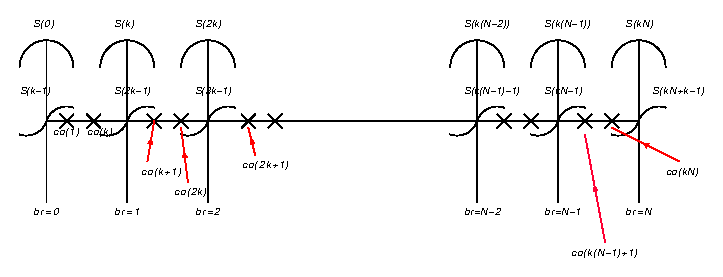
\includegraphics{splinemethod.eps}
%\caption{spline method explanation}
%\label{fig:spline}
%\end{figure}


미분 방정식을 푸는 방법에는 여러가지가 있지만, 3-body 이상의
partial differential equation의 경우에는 spline function을 
이용하여 eq.을 discrete matrix linear algebra equation으로 
바꾸는 것이 편리하다.

\subsection{Cubic Hermite spline}
\begin{figure}[h!]
\begin{center}
%\mbox{\epsfxsize=6cm\epsffile{CubicHermite.eps}}
\includegraphics[height=60mm]{CubicHermite1.png}
\end{center}
\caption{Cubic Hermite functions.}
\label{fig:spline}
\end{figure}
Spline method uses order $k$ spline functions for
interpolation of function and discretization
of equation. This is better for 
interpolate function and its derivative, thus
suitable for differential equation.
Cubic Hermite spline interpolation in interval $(x_i,x_{i+1})$
can be written for function $y=f(x)$, 
\bea
f(x)=h_{00}(t)y_i+h_{10}(t)(x_{i+1}-x_i)m_i
    +h_{01}(t)y_{i+1}+h_{11}(t)(x_{i+1}-x_i) m_{i+1} 
\eea 
where, $t=(x-x_i)/(x_{i+1}-x_i)$ and 
$m_i$ is a value of tangent function at point $x_i$.
Basis functions are given as
\begin{equation}
\begin{array}{l|l|l}
           &\mbox{ expanded}& \mbox{factorized} \\
           \hline 
 h_{00}(t)=S_{2i}(t) & 2t^3-3t^2+1    & (1+2t)(1-t)^2     \\
 h_{10}(t)=S_{2i+1}(t) & t^3-2t^2+t     & t(1-t)^2          \\
 h_{01}(t)=S_{2(i+1)}(t) & -2t^3+3t^2     & t^2(3-2t)         \\
 h_{11}(t)=S_{2(i+1)+1}(t) & t^3-t^2        & t^2(t-1)\\
\end{array} 
\end{equation}
여기서, tangent function $m$ is not unique.
Let us choose here $m_i=\frac{d}{dx}f({x=x_i})$
or numerically equivalent choices
\bea
m_i=\frac{y_{i+1}-y_{i-1}}{x_{i+1}-x_{i-1}},\mbox{ or }
m_i=\frac{y_{i+1}-y_i}{2(x_{i+1}-x_i)}
   +\frac{y_{i}-y_{i-1}}{2(x_{i}-x_{i-1})}.
\eea
따라서, $x_i<x<x_{i+1}$ 에서의 함수값을 interpolate하기 위해서는,
$y_{i-1},y_{i},y_{i+1},y_{i+2}$ 또는,
$y_{i},y'_i,y_{i+1},y'_{i+1}$ 의 4개의 함수 값이 필요하다. 

 We may rename basis functions as $S_{n}(x)$.
so that spline function $S_{2i}(x_i)=1$ and 
$S'_{2i+1}(x_i)=1$.
그러면, $x_i<x<x_{i+1}$ 에서
\bea
f(x)=C_{2i} S_{2i}(x)+C_{2i+1}S_{2i+1}(x)+C_{2i+2}S_{2i+2}(x)
    +C_{2i+3}S_{2i+3}(x)
\eea
으로 interpolation 하게 된다. 이 때, $S_{2i}(x)$ and $S_{2i+1}(x)$
는 $x_{i-1}<x<x_{i+1}$ 사이에서 정의되는 함수이다.(단, 경계에서는
$S_{0,1}(x)$는 $x_0<x<x_1$에서 정의된 함수.)이고, spline coefficient
$C_{2i}=y_i$ and $C_{2i+1}=y'_i$ 로 결정된다.

Thus, $S_{2i}(x)$ and $S_{2i+1}(x)$ is defined as
\begin{equation}
\begin{array}{c|c|c|c}
      &  x_{i-1}<x<x_i & x_i<x<x_{i+1} & \mbox{C}\\ \hline
  t   & \frac{x-x_{i-1}}{x_i-x_{i-1}},\ t=(0,1) 
      & \frac{x-x_i}{x_{i+1}-x_i},\ t=(0,1) 
      & \\
  S_{2i}(x) & t^2(3-2t)    & (1-t)^2(1+2t) & C_{2i}=y_i\\
  S_{2i+1}(x) & -(x_i-x_{i-1})t^2(1-t) & (x_{i+1}-x_i)t(1-t)^2 
              & C_{2i+1}=y'_i\\
\end{array}
\end{equation}
Thus, given list of break points and values of $y_i$ and $y'_i$
at break points determines all spline functions and 
its coefficients.


\subsection{Discretizing Differential equation}
미분 방정식
$$\hat{L} F(r)=0 $$ 을 푸는 경우, $0\ge r\ge r_N$ can be interpolated as
\bea
F(r)\simeq \sum_{j=0}^{k(N+1)-1} C_j S_j(r).
\eea
하지만, 동시에 미분 방정식을
matrix로 바꾸기 위해서는 $r$ 을 mesh points로 나누어야 한다.
이 경우 mesh points를 각 break point 사이의 interval 에 대한
legendre quadrature로 잡는 것이 편리하다.

 spline function 의 index는
전체 구간을 $x_0,..,x_N$ 의 break point로 나누었을 때,
각 break point마다 k 개의 spline function이 배당되는
식으로 정한다. 그리고, 각 interval,$[x_i,x_{i+1}]$ , 
에서 non-zero인 spline function은 break point
$x_i$와 $x_{i+1}$ 에 해당하는 spline function뿐이다.  
그러면, differential equation은
\bea
\sum_{j=0}^{k(N+1)-1} C_j [\hat{L} S_j(r)]=0
\eea
으로 바뀌고, 우리는 total $k(N+1)$개의 unknown coefficient
$C_j$를 구해야한다. 이 때, collocation point $col_1,..col_{kN}$ 
point에서의 식들을 independent 하게 취급하여, $KN$ 개의
식을 얻을 수 있다. 나머지, k 개의 조건은 boundary 
condition으로부터 얻을 수 있다.
예를 들어, $k=2$ 인 경우 boundary condition에 의해서,
$C_0,C_1,...,C_{2N},C_{2N+1}$ 중에
\bea
& &F(r=0)=0=C_0\no
& &F(r=r_N)=C_{2N} 
\eea
으로 $C_0$와 $C_{2N}$가 미리 결정된다. 
따라서, k-개의 boundary condition 을 포함하여, 
\bea
\sum_{j=0}^{k(N+1)-1} C_j [\hat{L} S_j(r_i)]=0,\mbox{
 $i$ 는 $1,2,\dots,k(N+1)$}
\eea
의 식이 얻어진다. 그리고, $[\hat{L} S_j(r_i)]\to [A]_{i,j}$
로 matrix로 나타내면,
\bea
[A]c=0
\eea
의 linear algebra problem 으로 바뀐다. 여기서,
$[A]$ 와 $c$ 는 dimension 이 $k(N+1)$ 으로 쓰거나,
이미 $k$ 개의 $C$ 가 결정되어 있으므로, $kN$ 만의 
식으로 쓸 수 있다. 단, $kN$ 개 coefficient 만의
식을 쓸 경우, bound state라면, 나머지 모든 coefficient가 
zero 이므로, 새로운 term 이 나타나지 않지만,
scattering state의 경우에는 boundary condition에 의해서,
\bea
[A]c=b
\eea
와 같이 boundary 에서의 coefficient 에 비례하는 
term 이 나타나게 된다.
이 때, 
\bea
[b]_i=-\sum_{j=kN+1}^{k(N+1)-1} C_j[\hat{L} S_j(r_i)],
\mbox{ i 는 $kN+1,\dots,k(N+1)$}
\eea
이고, $C_j$는 boundary 즉 last break point 에서의 
$F(r_N)$ 및 그 derivative 에 의해서,
\bea
C_{kN}=F(r=r_N),\quad C_{kN+1}=F'(r=r_N),\dots
\eea
결정된다. 

실제 계산에서는 boundary condition 을 $r=0$ 과
$r=r_{max}$ 에서의 값으로 주는 것이 보통이다. 
이런경우에는 
식을 어떻게 써야할까? 
\bea
F(r)\simeq \sum_{j=0}^{k(N+1)-1}C_j S_j(r)
     =\sum_{j=1}^{kN} C_j S_j(r)
     +\sum_{j=kN+1}^{kN+k-1} C_j S_j(r)    
\eea
이고, 특히 $k=2$인 경우는, $C_0=0$인 경우 $(F(0)=0)$
\bea
F(r)&=&\sum_{j=1}^{2N-1} C_j S_j(r)
       +C_{2N}S_{2N}(r)+C_{2N+1}S_{2N+1}(r)   
\eea
로 쓸 수 있고, 이 중 $C_{2N}$은 boundary condition
에 의해서, $C_{2N}=F(r=r_N)$ 으로 이미 결정되어 있다.
따라서, 마지막 2개의 spline coefficient 및
spline function의 이름을 바꾸어, 
\bea
F(r)=\sum_{j=1}^{kN} \tilde{C}_j \tilde{S}_j(r)
       +F(r_N)\tilde{S}_{2N+1}(r) ,   
\eea
where
\bea 
C_{2N}S_{2N}(x)=\tilde{C}_{2N+1}\tilde{S}_{2N+1}(x),\quad
C_{2N+1}S_{2N+1}(x)=\tilde{C}_{2N}\tilde{S}_{2N}(x),
\eea 

형식으로 쓸 수 있다. 단, 이경우, 마지막 
spline function
$\tilde{S}_{2N}(r), \tilde{S}_{2N+1}(r)$ 은 
실제로는 $S_{2N+1}(r), S_{2N}(r)$ 이고,
$\tilde{C}_{2N}$ 은 $F'(r_N)$에 해당한다는 점에 주의할 것. 만약, bound state
였다면, 위 식에서 마지막, $\tilde{S}_{2N+1}(r)$의 coefficient를 zero
로 둘 수 있게 된다. 따라서, $C_{1\dots 2N}$ 의 unknown
coefficients를 구하는 문제로 바뀐다.
따라서, collocation points $r_1,\dots r_{2N}$ 에 대한 식은
\bea
\hat{L}F(r_i)=\sum_{j=1}^{2N}[\hat{L}\tilde{S}_j(r_i)]C_j
              +F(r_N)\hat{L}\tilde{S}_{2N+1}(r_i)=0
\to \sum_j [A]_{ij}[C]_j +[B]_i=0  
\eea
으로 쓸 수 있게 된다. 2차 미방의 경우, we can have two solutions,
$[C^{(1)}]_j$ and $[C^{(2)}]_j$ 를 2개의 boundary condition
으로 부터 구할 수 있고, normalization factor는 boundary condition과의
matching 으로 구할 수 있다.

하지만, scattering problem 에서는 asymptotic wave function 
의  phase shift/K-matrix 가
미리 알려져 있지 않기 때문에 $F(r_N)$ 을 미리 결정해서 줄 수가 없다. 
만약 전체 미방이 homogeneous 라면, 미리, $F(r_N)=1$ 으로
scale 된 문제를 푼 다음에, K-matrix 를 나중에 구해서 다시 보정할 할 수 있을 것이다. 
\bea
\phi_{\alpha}(r)\sim \frac{[j_\alpha(kr)\delta_{\alpha\beta}
                    -K_{\alpha\beta} n_\beta(kr)]}
                    {[j_\alpha(kr_N)\delta_{\alpha\beta}
                    -K_{\alpha\beta} n_\beta(kr_N)]}
                    \to\ C_{2N}=1
\eea
$r_{match}<r_N$ 에서의 solution을 이용하여 matching 
하면 K-matrix를 결정할 수 있고, 따라서, 거꾸로 $C_{2N}=F(r_N)$ 을 다시 
보정해 줄 수 있다.     

Inhomogeneous equation의 경우에도 풀어야하는 방정식 자체는 비슷하다. 
Scattering 문제의 경우에는 $[B]_j$ 안에 inhomogeneous term 이 포함되게 된다. 
문제는 Inhomogeneous equation에서는 $F(r_N)$ 을 임의로 
scale 할 수 없을 것이라는 점이다. 
Boundary condition을 어떻게 주어야 할까? 이 경우에는 
asymptotic boundary conditiond르 이용하여 $F(r_N)$ 이 
$F'(r_N)$의 함수가 되도록 만들면, equation에서 $F(r_N)$ 을 없앨 수가 있다.  
예를 들어 asymptotic form 이 $S*g(r)$ 로 unknown $S$ 를 포함하더라도 ,
logarithmic derivative continuous condition은 
\bea 
\frac{F'(r=r_N)}{F(r=r_N)}=\frac{g'(r=r_N)}{g(r=r_N)}
\eea 
이 되어 matrix equation에서 $F(r_N)$ 대신 $F'(r_N)$을 사용할 수 있게 된다. 

\subsubsection{Converting collocation point values to spline coefficient}

한편, 주어진 collocation points value들로 부터 spline coefficient를 역으로
구하는 것은

\bea
F(r_i)=\sum_{j=0}^{2N+1} C_j S_j(r_i)
      =\sum_{j=1}^{2N} \tilde{C}_j \tilde{S}_j(r_i) 
                     +F(r_N)\tilde{S}_{2N+1}(r_i)
\eea 
로 쓸 수 있다. 따라서, matrix를
$S_{ij}=S_j(r_i)$ 로 정의하면,
\bea
C_j=\sum_{i=0}^{2N+1} [S^{-1}]_{ji} F(r_i),\mbox{ or }
\tilde{C}_j=\sum_{i=1}^{2N}[\tilde{S}^{-1}]_{ji}
                [F(r_i)-F(r_N)\tilde{S}_{2N+1}(r_i)]
\eea
로 구할 수 있다.

\subsubsection{예}
간단한 예를 들어 보자. 문제를 단순히 하기 위해서, cubic hermite polynomial (k=2)
경우이고 구간이 단순히 $x_0$ 와 $x_1$ 인 경우만 생각해보자. 이 구간에서
임의의 함수값은
\bea
f(r)\simeq C_0 S_0(r)+C_1 S_1(r)+C_2 S_2(r)+C_3 S_3(r)
\eea
으로 정해진다. boudary condition에 의해서 4 개의 coefficient 중 오직 
2개만이 unknown 이된다. 미분 방정식도
\bea
[L]f(r)=C_0 [L]S_0(r)+ C_1[L]S_1(r)+ C_2 [L]S_2(r)+ C_3 [L] S_3(r)=[B](r)
\eea
로 주어진다. 경계 조간에 따라서, 풀어야하는 선형방정식이 달라지게 된다.
예를 들어 $f(x_0)=0$, $f(x_1)=0$(or $C_0=C_2=0$ 
의 2-boundary value가 주어지는 경우.
두 점 $r_1, r_2$ 에서 다음을 풀면된다.
\begin{equation}
\left(\begin{tabular}{cc} $[L]S_1(r_1)$ & $[L]S_3(r_1)$ \\
                          $[L]S_1(r_2)$ & $[L]S_3(r_2)$ \end{tabular}
\right)\left( \begin{tabular}{c} $C_1$ \\ $C_3$ \end{tabular}\right)
=\left( \begin{tabular}{c} $[B](r_1)$ \\ $[B](r_2)$ \end{tabular}\right)
\end{equation}

비슷하게, 만약 함수의 collocation points 에서의 값이 주어져 있을 때,
spline coefficient는 다음과 같이 구할 수 있다.
\bea
f(r_1)&=& C_1 S_1(r_1)+ C_3 S_3(r_1),\no
f(r_2)&=& C_1 S_1(r_2)+ C_3 S_3(r_2)
\eea
because $C_0=0$ and $C_2=0$ is already known.

\subsection{Explicit form of matrix equation}
Differential equation we would like to solve is
\bea 
\left[ -\frac{1}{2\mu}\frac{d^2}{dx^2}+\frac{1}{2\mu}\frac{l'(l'+1)}{x^2}-E\right] 
u_{l' l}(x)+\sum_{\beta} x V_{l'\beta}(x) \frac{u_{\beta l}(x)}{x} =0
\eea 
With using last term exchanged spline function $\tilde{S}_j(x)$,
we will interpolate
\bea 
u_{\alpha\beta}(x)&=&\sum_{j=0}^{2N+1}\tilde{C}_{\alpha,j}^{\beta} \tilde{S}_j(x) \no 
                  &=&\sum_{j=1}^{2N} \tilde{C}_{\alpha,j}^{\beta} \tilde{S}_j(x)
                  +\tilde{C}_{\alpha,0}^{\beta} \tilde{S}_0(x)
                  +\tilde{C}_{\alpha,2N+1}^{\beta} \tilde{S}_{2N+1}(x)
\eea 
Then, above equation becomes
\bea 
& &\sum_{\beta=1}^{N_{s}}\sum_{j=0}^{2N+1} 
\left[-\frac{1}{2\mu}\frac{d^2}{dx^2}\tilde{S}_j(x)\delta_{l',\beta}
     +\frac{1}{2\mu}\frac{l'(l'+1)}{x^2}\tilde{S}_j(x)\delta_{l',\beta}-E\tilde{S}_j(x)\delta_{l',\beta}
     \right]
     \tilde{C}_{\beta,j}^{l} \no 
& &+\sum_{\beta=1}^{N_{s}}\sum_{j=0}^{2N+1}
 \left[x V_{l'\beta}\frac{\tilde{S}_j(x)}{x} \right]\tilde{C}_{\beta,j}^{l} =0
\eea 
By choosing $x_i$ points, $i\in[1,2N]$, 
we can have $2N$ number of equations.
Let us define vectors and matrices as
\bea 
[\tilde{C}^l]_{n}&\equiv& \tilde{C}^l_{\beta,j} ,
\eea
\bea 
[\Delta]_{n'n}&\equiv& 
         -\frac{1}{2\mu}\frac{d^2}{dx^2}\tilde{S}_j(x_i)\delta_{l',\beta}
              +\frac{1}{2\mu}\frac{l'(l'+1)}{x_i^2}\tilde{S}_j(x_i)\delta_{l',\beta},   
\eea 
\bea 
[B]_{n'n}&\equiv& \tilde{S}_j(x_i) \delta_{l'\beta}, 
\eea 
\bea 
[V]_{n'n}&\equiv& x_i V_{l'\beta}(x_i)\frac{\tilde{S}_j(x_i)}{x_i}, 
\eea 
with
\bea 
n'\equiv(l',i) \mbox{ and }  n\equiv(\beta,j),
\eea 
Then, above equation can be rewritten as matrix equation,
\bea 
\sum_{\beta=1}^{N_{s}}\sum_{j=0}^{2N+1}[\Delta -E B +V]_{n'n}[\tilde{C}^l]_n=0.
\eea 
Note that number of index is different between $n'$ and $n$. 
We have to use boundary conditions to make the above equation to be 
square. 

Let us denote $n_0\equiv(\beta,0)$ and $n_f\equiv(\beta,2N+1)$ and separate
\bea 
\sum_{\beta=1}^{N_{s}}\sum_{j=1}^{2N}[\Delta -E B +V]_{n'n}[\tilde{C}^l]_n
+\sum_{\beta=1}^{N_{s}}[\Delta -E B +V]_{n'n_0}[\tilde{C}^l]_{n_0}
+\sum_{\beta=1}^{N_{s}}[\Delta -E B +V]_{n'n_f}[\tilde{C}^l]_{n_f}
=0.
\eea 
For bound state problem, we can use boundary condition as
\bea 
[\tilde{C}^l]_{n_0}=0,\quad [\tilde{C}^l]_{n_f}=0, \mbox{ for all }\beta. 
\eea  
and the matrix equation becomes eigenvalue problem
\bea 
{\sum_{n}}'[\Delta+V]_{n'n}[\tilde{C}^l]_n=E{\sum_{n}}'[B]_{n'n}[\tilde{C}^l]_n,
\quad \mbox{ with } {\sum_{n}}'\equiv \sum_{\beta=1}^{N_s}\sum_{j=1}^{2N}.
\eea 

For the scattering case, we have to use asymptotic form of wave function as boundary 
condition,
\bea 
[\tilde{C}^l]_{n_0}=0,\quad 
[\tilde{C}^l]_{n_f}= u_{\beta l}(r=r_N)
                   =\frac{1}{2}r[\delta_{\beta l} h_{\beta}^{(-)}(kr)
                                 +S_{\beta l} h_{\beta}^{(+)}(kr)]   
.
\eea 
and the matrix equation becomes
\bea 
{\sum_{n}}'[\Delta+V-E B]_{n'n}[\tilde{C}^l]_{n}
=[ G^l ]_{n'},
\quad [G^l]_{n'}\equiv -\sum_{\beta=1}^{N_{s}}[\Delta -E B +V]_{n'n_f}[\tilde{C}^l]_{n_f}
\eea 

But, in fact, asymptotic form of $u_{\beta l}$ contains unknown 
complex S-matrix. Because of homogeneous form of the equation, 
we can change normalization of solution. 
However, still it does not completely fix boundary condition if it is a coupled equation.
How should we solve the problem? 

{\bf Possible answer?:} M원 N차 연립 미분 방정식의 general solution은 
M*N 개의 independent boundary condition을 통해 얻은 M*N개 
solution들의 선형 결합으로 표현된다? 만약 이 주장이 옳다면, 위 문제에서 
regular solution 에 한정해서, $[\tilde{C}^l]_{nf}=\delta_{\beta l}$ 
로 모든 $l=1..N_s$ 개의 different boundary condition으로 부터  
$N_s$ 개의 solution을 구한다음 이것들이 어떻게 결합하여 원하는 boundary condition을 줄 수 있는지
구하면 된다. So, we will let 
\bea 
[G^l]_{n'}\equiv -\sum_{\beta=1}^{N_{s}}[\Delta -E B +V]_{n'n_f} \delta_{\l \beta}
             = -[\Delta -E B +V]_{n'(l,2N+1)}
\eea 
And solve for different $l$'s and get $N_s$ different solutions. Then, 
recombine them to obtain asymptotic boundary condition and fix the S-matrix. 

Suppose we obtained $[\tilde{C}^{l=1..N_s}]_{i=1..2N}$. Then how can we find the
correct normalization and S, K matrix?


\subsection{Special case: perturbation}
In case of inhomogeneous PV equation, 
\bea 
\left[ -\frac{1}{2\mu}\frac{d^2}{dx^2}+\frac{1}{2\mu}\frac{l'(l'+1)}{x^2}-E\right] 
u^{PV}_{l' l}(x)+\sum_{\beta} x V^{PC}_{l'\beta}(x) \frac{u^{PV}_{\beta l}(x)}{x}
+\sum_{\beta} x V^{PV}_{l'\beta}(x) \frac{u^{PC}_{\beta l}(x)}{x}
 =0,
\eea
we can transform the equation into matrix equation,
\bea 
& &\sum_{\beta=1}^{N_{s}}\sum_{j=1}^{2N}[\Delta -E B +V^{PC}]_{n'n}[\tilde{C}^{PV,l}]_n \no 
& &+\sum_{\beta=1}^{N_{s}}[\Delta -E B +V^{PC}]_{n'n_0}[\tilde{C}^{PV,l}]_{n_0}
+\sum_{\beta=1}^{N_{s}}[\Delta -E B +V^{PC}]_{n'n_f}[\tilde{C}^{PV,l}]_{n_f} \no 
& &+\sum_{\beta=1}^{N_s}\sum_{j=0}^{2N+1}[V^{PV}]_{n'n}[\tilde{C}^{PC,l}]_{n} 
=0.
\eea  
Suppose we already solved the parity conserving wave function, 
the last term is already known and we can write as
\bea 
[K^l]_{n'} \equiv -\sum_{\beta=1}^{N_s} x_i V^{PV}_{l'\beta}(x_i) \frac{u^{PC}_{\beta l}(x_i)}{x_i}
\eea 

However, the boundary condition for $u^{PV}$ as   
\bea 
[\tilde{C}^{PV,l}]_{n_0}=0, \quad [\tilde{C}^{PV,l}]_{n_f}=u^{PV}_{\beta l}(r=r_N),
\eea 
is not directly applicable because it contains unknown scattering matrix
and also cannot be arbitrarily scaled,
\bea 
u^{PV}_{\beta l}(r)=\frac{1}{2}S^{PV}_{\beta l} h^{(+)}_{\beta}(kr),
\eea 
where there is no $\delta_{\beta l}$ because $\beta\neq l$ for PV transition.
But we can use logarithmic derivative continuous condition,
\bea 
\frac{1}{u^{PV}_{\beta l}(r)}\frac{d u^{PV}_{\beta l}(r)}{dr}
=\frac{1}{ h^{(+)}_{\beta}(kr)}
 \frac{d h^{(+)}_{\beta}(kr)}{dr}
\eea 
Thus replace
\bea 
u^{PV}_{\beta l}(r=r_N)=\frac{h^{(+)}_{\beta}(kr_N)  }{ \frac{d }{dr}h^{(+)}_{\beta}(kr_N)} 
                       \frac{d u^{PV}_{\beta l}(r_N)}{dr}
                       =\frac{h^{(+)}_{\beta}(kr_N)  }{ \frac{d }{dr}h^{(+)}_{\beta}(kr_N)}
                       \tilde{C^l}_{\beta,2N} =\tilde{C^l}_{\beta,2N+1} 
\eea 
and change 
\bea 
& &\sum_{\beta=1}^{N_{s}}[\Delta -E B +V]_{n'n_f}[\tilde{C}^{PV,l}]_{n_f} \no 
&+&\sum_{\beta=1}^{N_s}\sum_{j=1}^{2N} \left[ \delta_{j,2N}
   [\Delta-E B+V^{PC}]_{n',n_f} 
   \left(\frac{h^{(+)}_{\beta}(kr_N)  }{ \frac{d }{dr}h^{(+)}_{\beta}(kr_N)}\right) 
   \right] 
   [\tilde{C}^{PV,l}]_{n} \no 
&\equiv& {\sum_{n}}'[X]_{n'n}[\tilde{C}^{PV,l}]_{n}   
\eea 
And finally the equation becomes
\bea 
{\sum_n}' [\Delta+V^{PC}- E B+X]_{n'n}[\tilde{C}^{PV,l}]_{n}=[K^l]_{n'}
\eea 
After obtaining $[\tilde{C}^{PV,l}]_{n}$, we can obtain 
\bea 
S^{PV}_{\beta l}=\frac{ 2 \tilde{C}^{PV,l}_{\beta,2N} }{ \frac{d }{dr}h^{(+)}_{\beta}(kr_N)}
\eea 

One subtle point in above expression is that $\beta$ must contain 
both parity even and parity odd states. For example we choose
$l'=1$ and $l=0$, $\sum_{n}$ in the above matrix equation 
must be parity odd states but $\sum_{\beta}$ in $[K]$ must be parity even states.
Also, we have to solve the matrix equation for complex coefficients, unlike Parity conserving case.

\subsection{Practical implementation }
먼저, potential 이 real인 경우, complex normalization factor를 밖으로 빼어내서, 
우리는 언제나 real-valued solution을 얻을 수 있다. scattering state의 경우에는 complex 
normalization factor 를 
\bea
\label{spline:interp} 
R_{\alpha',\alpha}(x)=\sum_{\beta} \hat{R}_{\alpha',\beta}(x)[\frac{1+\hat{S}}{2}]_{\beta\alpha},
\no 
\hat{R}_{\alpha',\beta}(x)\to \delta_{\alpha',\beta} j_{L'}(kx)
                             -\hat{K}_{\alpha'\beta} n_{L'}(kx) 
\eea 
로 빼낼 수 있고, normalization 은 
\bea 
\label{spline:SK}
[\frac{1+\hat{S}}{2}]_{\beta\alpha}=[(1-i\hat{K})^{-1}]_{\beta,\alpha}
\eea 
을 이용해  K-matrix로 나타낼 수 있다. 

한편, 실제 계산에서 우리가 다루는 것은 spline coefficient 에 관한 equation이다. 따라서, 
\bea 
\hat{R}_{\alpha,\beta}(x)=\sum_{j=1}^{2N_x} \tilde{C}^{\beta}_{\alpha,j} \tilde{S}_j(x)
                           +\tilde{C}^{\beta}_{\alpha,2N_x+1} \tilde{S}_{2N_x+1}(x)
\eea 
이것은 위의 K-matrix 와 다음 식을 만족해야 한다. 
\bea 
\tilde{C}^{\beta}_{\alpha,2N+1}&=& \hat{R}_{\alpha,\beta}(x_N)
                                 =\delta_{\alpha,\beta} j_{\alpha}(kx_N)
                                 -\hat{K}_{\alpha\beta} n_{\alpha}(kx_N),\no  
\tilde{C}^{\beta}_{\alpha,2N}&=& \hat{R}'_{\alpha,\beta}(x_N)
                                 =\delta_{\alpha,\beta} j'_{\alpha}(kx_N)
                                 -\hat{K}_{\alpha\beta} n'_{\alpha}(kx_N).
\eea 
따라서, 
\bea 
\label{spline:last}
K_{\alpha\beta}&=&\left[
    \frac{\delta_{\alpha\beta}j'_\alpha(kx_N)-\tilde{C}^{\beta}_{\alpha,2N}}
    {n'_\alpha(kx_N)}      \right],
\no 
\tilde{C}^{\beta}_{\alpha,2N+1}&=&
 \left[\delta_{\alpha,\beta} j_{\alpha}(kx_N)
       -\delta_{\alpha\beta}\frac{n_\alpha(kx_N)}{n'_\alpha(kx_N)} j'_{\alpha}(kx_N)\right] 
   +\tilde{C}^\beta_{\alpha,2N} \frac{n_\alpha(kx_N)}{n'_\alpha(kx_N)}    
\eea 
으로 $\tilde{C}^\alpha_{\beta,(2N)}$ 값으로 모두 나타낼 수 있다. 따라서, linear algebra 문제를 
푸는데 두 가지 접근을 생각해 볼 수 있다. eq.(\ref{spline:interp})에 eq.(\ref{spline:last})를 
대입하여, 식을 $\tilde{C}^\alpha_{\beta,1:2N}$ 에 대한 inhomogeneous equation으로 만들어서 
풀면, normalization condition까지 고려한 결과 $\tilde{C}^\alpha_{\beta,1:2N}$를 한 번에 
얻게 된다. 한 편, 위와 같이 푸는 대신, 
$\tilde{C}^\beta_{\alpha,2N+1}=\delta_{\alpha,\beta}$의 boundary condition 을 주어 
모든 $\beta$ 에 대한 solution을 얻은 뒤 다시 normalization을 restore 해주는 방법이다. 
이렇게 구해진 spline coefficient solution을 $D^\beta_{\alpha,j}$ 라고 하자. 
즉, 우리는 
\bea 
\label{spline:CD}
\tilde{C}^\beta_{\alpha,j}=\sum_{\gamma} M_{\alpha\gamma}\tilde{D}^\gamma_{\beta,j}
,\quad 
\tilde{D}^\beta_{\alpha,2N+1}= \delta_{\alpha,\beta},
\quad 
\eea 
인 solutions $\tilde{D}^\beta_{\alpha,j}$ 를 얻었다고 하자. 
Conversion factor or Normalization factor $M_{\alpha\gamma}$ can be obtained from
the comparison with eq.(\ref{spline:last}), $M_{\alpha\beta}=\tilde{C}^\beta_{\alpha,2N+1}$.
하지만, $\tilde{C}$ 는 미리 알려진 것이 아니므로, M 을 D로 나타내어 주면,\footnote{
It is possible that the number of interested coupled channels is less than 
the number of internal partial wave states. In that case, matrix M can be non-square.
But, nonetheless the equation can be solved.
$ [M(N_s\times N_{ch}) [D(N_{ch}\times N_s)]=[N_s\times N_s]$, which can be 
changed into the form of $Ax=b$ by transpose the equation. 

}
\bea 
\label{spline:M}
\sum_{\gamma} M_{\alpha\gamma}\left[\tilde{D}^\gamma_{\beta,2N+1}-
                        \tilde{D}^\gamma_{\beta,2N}\frac{n_\alpha(kx_N)}{n'_\alpha(kx_N)}\right] 
 =\left[\delta_{\alpha,\beta} j_{\alpha}(kx_N)
        -\delta_{\alpha\beta}\frac{n_\alpha(kx_N)}{n'_\alpha(kx_N)} j'_{\alpha}(kx_N)\right]  
\eea  
으로부터 , $M_{\alpha\gamma}$를 구할 수 있다. Note here $\gamma=1:N_{ch}$ but $\alpha,\beta=1:N_s$.

In summary, the steps we need to takes are
\begin{enumerate}
\item Solve and obtain solutions for coupled channels
      $\tilde{D}^\gamma_{\alpha, j}$ for $j=1:2N$ 
      with boundary conditions
      $\tilde{D}^\beta_{\alpha,2N+1}= \delta_{\alpha,\beta}$. 

\item Obtain conversion matrix $M$ from eq.(\ref{spline:M} ).

\item Obtain $\tilde{C}$ from eq. (\ref{spline:CD}).

\item Obtain $K$-matrix and last spline coefficients from eq.(\ref{spline:last})

\item Obtain complex normalization and S-matrix from eq.(\ref{spline:SK})

\item Finally, full wave function can be obtained 
      by multiplying complex normlaization to real valued solutions. 
 
\end{enumerate}

Until now we used notation $n=(\beta,j)$ 
to represent both partial wave quantum number and
spatial coordinate ot spline index. In practical implementation, it would be better
to introduce 1-D index
\bea 
k=(\beta-1)*(k N_x)+j, \quad \beta=1\dots N_s,\quad j=1\dots k N_x,
\eea 
so that the wave function $F_{\alpha,i}(x)$ can be written as 1-D array
$F_i(k=1\dots N_s k N_x)$ with only external index for initial channel $i$.
If we have coupled channels, we would want match 
\bea 
F^{full}_i(1:N_s k N_x)=\sum_j N_{ij} F^{num}_{j}(1:N_s K N_x),
\eea   
where, $F^{full}_i(1:N_s k N_x)$ is a full complex wave function with correct 
normalization and asymptotic form in channel $i$,
$F^{num}_{j}(1:N_s K N_x)$ is a numerical solution with boundary 
condition of $[\tilde{C}^j]_{nf}=\delta_{\beta j}$ and $N_{ij}$
is a complex normalization matrix to match $F^{full}_i$. 


\subsection{Lanczos method: iteration method}
앞에서 3-body 문제를 spline method를 이용하여
linear algebra 문제로 바꾸는 것을 살펴보았다.
여기서는 linear algebra problem 특히 bound state의 경우에
large matrix에 대해 효율적으로 푸는 방법을 살펴보자. 이것은 다음 3-body 노트에서 이야기하자.


\newpage
\section{T-amplitude with two different potential
(Alternate derivation of DWBA)
}
Let us call there are two potentials 
$\hat{V}=\hat{V}_Y+\hat{C}$.
In operator form, the T matrix will be written as
\bea
\hat{T}=\hat{V}+\hat{V}\hat{G}_0\hat{T}
       =\hat{V}+\hat{V}\hat{G}\hat{V} 
\eea
We introduce Green's functions and $\hat{T}_Y$ as
\bea
& &\hat{G}^{(+)}=\frac{1}{E-\hat{H}_0-\hat{V}+i\epsilon},\quad
\hat{G}^{(+)}_0=\frac{1}{E-\hat{H}_0+i\epsilon},\quad
\hat{G}^{(+)}_Y=\frac{1}{E-\hat{H}_0-\hat{V}_Y+i\epsilon},\no
& &\hat{T}_Y=\hat{V}_Y+\hat{V}_Y\hat{G}_0\hat{T}_Y
            =\hat{V}_Y+\hat{V}_Y\hat{G}_Y\hat{V}_Y  
\eea
From the relation between Green's functions, we get formal relations
\footnote{In general, we can use matrix relations 
\bea
B(1-AB)^{-1}=(1-BA)^{-1}B, \quad
(1-A)^{-1}=1+A(1-A)^{-1},\quad
A(1-A)^{-1}=(1-A)^{-1}A
\eea
}
\bea
\hat{G}^{-1}&=&\hat{G}_Y^{-1}-\hat{C},\no
\hat{G}&=&(\hat{G}_Y-\hat{C})^{-1}
        =(1-\hat{G}_Y\hat{C})^{-1}\hat{G}_Y
        =\hat{G}_Y(1-\hat{C}\hat{G}_Y)^{-1},\no
\hat{C}\hat{G}&=& (1-\hat{C}\hat{G}_Y)^{-1}-1
      =(1-\hat{C}\hat{G}_Y)^{-1}\hat{C}\hat{G}_Y.   
\eea
Then, 
\bea
\hat{T}&=&(\hat{V}_Y+\hat{C})
          +(\hat{V}_Y+\hat{C})\hat{G}(\hat{V}_Y+\hat{C})\no
       &=&\hat{V}_Y+\hat{C}
          +\hat{V}_Y\hat{G}\hat{V}_Y
          +\hat{C}\hat{G}\hat{V}_Y
          +\hat{V}_Y\hat{G}\hat{C}
          +\hat{C}\hat{G}\hat{C}
\eea
we can replace
\bea
\hat{V}_Y\hat{G}\hat{V}_Y
&=&\hat{V}_Y\hat{G}_Y(1-\hat{C}\hat{G}_Y)^{-1} \hat{V}_Y
 =\hat{V}_Y\hat{G}_Y[1+\hat{C}\hat{G}_Y(1-\hat{C}\hat{G}_Y)^{-1}]\hat{V}_Y
 \no
 &=&\hat{V}_Y\hat{G}_Y\hat{V}_Y
    +\hat{V}_Y\hat{G}_Y(1-\hat{C}\hat{G}_Y)^{-1}\hat{C}\hat{G}_Y\hat{V}_Y,\no
\hat{C}\hat{G}\hat{C}
     &=&   (1-\hat{C}\hat{G}_Y)^{-1}\hat{C}-\hat{C},\no 
\hat{C}\hat{G}\hat{V}_Y
 &=&(1-\hat{C}\hat{G}_Y)^{-1}\hat{C}\hat{G}_Y\hat{V}_Y,\no
\hat{V}_Y\hat{G}\hat{C}
     &=&\hat{V}_Y\hat{G}_Y(1-\hat{C}\hat{G}_Y)^{-1}\hat{C}
\eea
Thus, we get
\bea
\hat{T}=\hat{T}_Y+
(1+\hat{V}_Y\hat{G}_Y)(1-\hat{C}\hat{G}_Y)^{-1}\hat{C}
(1+\hat{G}_Y\hat{V}_Y)
\eea
We define $|\chi_\vp\ra$ such that $|\chi_\vp\ra$
is a solution of Schrodinger equation for $\hat{V}_Y$:
\bea
|\chi_\vp\ra^{(\pm)}&\equiv& (1+\hat{G}^{(\pm)}_Y\hat{V}_Y)|\vp\ra,\no
\hat{G}_Y(E_p)^{-1}|\chi_\vp\ra
&=&(E_p-\hat{H}_0-\hat{V}_Y)|\chi_\vp\ra
=(\hat{G}_Y^{-1}(E_p)+\hat{V}_Y)|\vp\ra=(E_p-\hat{H}_0)|\vp\ra=0
\eea
Thus,
\bea
\la \vp'|\hat{T}(E)|\vp\ra
=\la \vp'|\hat{T}_Y(E)|\vp\ra
 +{}^{(-)}\la \chi_{\vp'}|(1-\hat{C}\hat{G}_Y(E))^{-1}\hat{C}
  |\chi_{\vp}\ra^{(+)}
\eea
where $E$ is not neccessarily $E_p$ or $E_{p'}$ when they are not on-shell.
If $\hat{C}$ is perturbative case, we may approximate
$(1-\hat{C}\hat{G}_Y)^{-1}\simeq 1$, and we get 
DWBA approximation. Above equation corresponds to the equation (4.5) in {\bf D.B.Kaplan etal., NPB478(1996)629.}

We may express rewrite the operators in terms of $\hat{G}_0$ and $\hat{T}_Y$ from relation,
\bea
\hat{T}_Y&=&\hat{V}_Y+\hat{V}_Y\hat{G}_0\hat{T}_Y
         =\hat{V}_Y+\hat{V}_Y\hat{G}_Y\hat{V}_Y, \no 
1+\hat{G}_Y\hat{V}_Y&=& \hat{G}_Y\hat{G}^{-1},
\eea
\bea
|\chi_\vp\ra&=&(1+\hat{G}_Y\hat{V}_Y)|\vp\ra
            =(1+\hat{G}_0\hat{T}_Y)|\vp\ra,\no
(1-\hat{C}\hat{G}_Y)^{-1}\hat{C}
&=&(\hat{C}^{-1}-(1+\hat{G}_YV_Y)\hat{G}_0)^{-1}.             
\eea
This corresponds to the equation (9) of {\bf 
Long and Yang, PRC86(2012)024001.}

\section{Chiral EFT potential up to NLO}
Machleidt potential in momentum space has form,
\bea 
V(\vp',\vp)&=&V_C+\tau_1\cdot\tau_2 W_C\no
           &+&\left[V_S+\tau_1\cdot\tau_2 W_S\right]\vs_1\cdot\vs_2\no 
           &+&\left[V_{LS}+\tau_1\cdot\tau_2 W_{LS}\right]
           (-i{\bm S}\cdot(\vq\times\vk))  \no 
           &+&\left[V_T+\tau_1\cdot\tau_2 W_T\right]
           \vs_1\cdot\vq \vs_2\cdot\vq \no 
           &+& \left[V_{\sigma L}+\tau_1\cdot\tau_2 W_{\sigma L}\right]
           \vs_1\cdot(\vq\times\vk )\vs_2\cdot(\vq\times\vk ) 
\eea  
where,
\bea 
\vq=&\vp'-\vp                    & \mbox{ momentum transfer } ,\no 
\vk=&\frac{1}{2}(\vp'+\vp)       & \mbox{ average momentum } ,\no
{\bm S}=&\frac{1}{2}(\vs_1+\vs_2) & \mbox{ total spin } 
\eea 

The LO($Q^0$) chiral EFT potential involves one-pion exchange and 
contact terms. 
\bea
V_{1\pi}(\vp',\vp)=-\frac{g_A^2}{4f_\pi^2}
 \tau_1\cdot\tau_2
 \frac{\vs_1\cdot\vq \vs_2\cdot\vq}{\vq^2+m_\pi^2},
 \quad V^{(0)}=C_S+C_T\vs_1\cdot \vs_2.  
\eea
The NLO($Q^2$) chiral EFT,
\bea 
W_C&=&-\frac{L(q)}{384\pi^2 f_\pi^4}
     \left[ 4m_\pi^2(5 g_A^4-4 g_A^2-1)
            +q^2(23 g_A^4-10 g_A^2-1)
            +\frac{48 g_A^4 m_\pi^4}{\omega^2} 
     \right],\no 
V_T&=& -\frac{1}{q^2} V_S=-\frac{3 g_A^4 L(q)}{64\pi^2 f_\pi^4},   
\eea 
where,
\bea 
L(q)\equiv \frac{\omega}{q}\ln \frac{\omega+q}{2m_\pi},
\quad \omega\equiv \sqrt{4 m_\pi^2+q^2}.
\eea 
NLO contact potentials
\bea 
V^{(2)}(\vp',\vp )
&=& C_1q^2+ C_2 k^2
+(C_3 q^2+ C_4 k^2)\vs_1\cdot\vs_2 \no & & 
+C_5(-i{\bm S}\cdot (\vq\times\vk ))
+C_6(\vs_1\cdot\vq )
    (\vs_2\cdot\vq )
+C_7(\vs_1\cdot\vk )(\vs_2\cdot\vk )      
\eea 

Partial wave representation of the potential can be obtained by,
\bea 
V_{L'L}(p',p)=\int d\Omega_{\vp'}\int d\Omega_{\vp}
             Y^*_{L'}(\hat{\vp}') V(\vp',\vp)
             Y_{L}(\hat{\vp})
\eea 
Thus, if we do not include regulator, potentials in each partial wave
are 
\bea 
V^{(0)}(^1S_0)&=& 4\pi (C_S-3C_T)=\widetilde{C}_{^1S_0},\no 
V^{(0)}(^3S_1)&=& 4\pi (C_S+C_T)=\widetilde{C}_{^3S_1},\no 
V^{(2)}(^1S_0)&=& C_{1S_0} (p^{'2}+p^2)
               =4\pi (C_1+\frac{1}{4}C_2-3C_3-\frac{3}{4}C_4
                -C_6-\frac{1}{4}C_7 )(p^{'2}+p^2),\no 
V^{(2)}(^3P_0)&=& C_{^3P_0} p p'=\dots,\no 
V^{(2)}(^1P_1)&=& C_{^1P_1}pp'=\dots,\no
V^{(2)}(^3P_1)&=& C_{^3P_1}pp'=\dots,\no
V^{(2)}(^3S_1)&=& C_{^3S_1}(p^2+p^{'2})=\dots,\no
V^{(2)}(^3S_1-^3D_1)
&=& C_{^3S_1-^3D_1} p^2=\dots,\no 
V^{(2)}(^3P_2)&=& C_{^3P_2}p p'=\dots                  
\eea 


\end{document}
